\documentclass[a4paper,12pt]{report}

% My added packages
\usepackage{blindtext}
\usepackage{amsfonts}
%
\usepackage{enumitem}
\usepackage{pgfplots}
\usepackage{rotating}
\usepackage{gensymb}
\usepackage{tikz,tikz-3dplot}

%\usepackage{csvsimple}
\pgfplotsset{compat=1.16}

\usepackage{import}
\usepackage{placeins}
\usepackage{xcolor}
\usepackage{pgf}

% Page layout
\usepackage[left=2.5cm,right=2.5cm,top=2.5cm,bottom=2.5cm]{geometry}

% Font and text
\usepackage[english]{babel} %afrikaans,
\usepackage{microtype}
\usepackage{setspace}
\usepackage{lmodern}
\usepackage{siunitx}
\newcommand{\myemph}[1]{{\sffamily\bfseries#1}}
\sloppy
\onehalfspacing

% Headings
\usepackage[raggedright,sf,bf]{titlesec}
\usepackage[margin=\the\parindent,small,bf,sf]{caption}
\titlelabel{\thetitle.\ }
\titleformat{\chapter}[display]{\huge\bfseries\sffamily}{\chaptertitlename\ \thechapter}{15pt}{\Huge \raggedright}
\titlespacing*{\chapter}{0pt}{0pt}{40pt}  % remove spacing before chapter headings
\makeatletter
\let\originall@chapter\l@chapter
\def\l@chapter#1#2{\originall@chapter{{\sffamily #1}}{#2}}
\makeatother

%% Alternative headings using small-caps (comment out the top section)
%\usepackage[raggedright,bf]{titlesec}
%\usepackage[margin=\the\parindent,small,bf]{caption}
%\titlelabel{\thetitle.\ }
%\titleformat{\chapter}[display]{\huge\scshape}{\chaptertitlename\ \thechapter}{15pt}{\Huge \raggedright}
%\titlespacing*{\chapter}{0pt}{0pt}{40pt}  % remove spacing before chapter headings

% Table of contents
\let \savenumberline \numberline
\def \numberline#1{\savenumberline{#1.}}

% Figures
\usepackage{graphicx}
\usepackage{pdfpages}
\usepackage{subcaption}
\setlength{\abovecaptionskip}{7.5pt}  % spacing above and below captions
\newcommand*{\WaterMark}[2][0.2\paperwidth]{\AddToShipoutPicture*{\AtTextCenter{\parbox[c]{0pt}{\makebox[0pt][c]{\includegraphics[width=#1]{#2}}}}}}
% Mathematics
\usepackage[cmex10]{amsmath}
\usepackage{amssymb}
\usepackage{cancel}
\DeclareMathOperator*{\argmax}{arg\,max}
\newcommand{\T}{^\top}
\newcommand{\tr}{\textrm{tr}}
\renewcommand{\vec}[1]{\boldsymbol{\mathbf{#1}}}
\newcommand{\defeq}{\triangleq}
% Tables
\usepackage{booktabs}
\usepackage{tabularx}
\usepackage{multirow}
\newcommand{\mytable}{
    \centering
    \small
    \renewcommand{\arraystretch}{1.2}
    }
\renewcommand{\tabularxcolumn}[1]{m{#1}}
\newcolumntype{C}{>{\centering\arraybackslash}X}
\newcolumntype{L}{>{\raggedright\arraybackslash}X}

% Header and footer
\usepackage{fancyhdr}
\pagestyle{fancy}
\fancyhf{}
\renewcommand{\sectionmark}[1]{\markright{\normalsize \thesection.\ #1}}
\fancyhead[C]{\nouppercase{\textit{\rightmark}}}
\fancyhead[RO]{\thepage}
 \fancyhead[LE]{\thepage}  % double-sided printing
\fancyfoot{}
\setlength\headheight{14.5pt}
\renewcommand{\headrulewidth}{0pt}
\fancypagestyle{plain}{\fancyhead{}
                       \renewcommand{\headrulewidth}{0pt}
                       \fancyfoot[C]{\thepage}}

\newcommand\norm[1]{\left\lVert#1\right\rVert}
% Pseudo-code
\usepackage{algorithm}  % should go before \usepackage{hyperref}

% Table of contents and hyperlinks
\usepackage{hyperref}
\hypersetup{colorlinks=true,linktoc=all,citecolor=black,linkcolor=black}
\usepackage[nottoc]{tocbibind}

% Pseudo-code
\usepackage{algpseudocode}  % should go after \usepackage{hyperref}
\renewcommand{\thealgorithm}{\arabic{chapter}.\arabic{algorithm}} 
\captionsetup[algorithm]{labelfont={bf,sf},font=small,labelsep=colon}

% Bibliography
% \usepackage[backend=biber]{biblatex}

\usepackage{cite}  % automatically reorder inline citations

\bibliographystyle{IEEEtran}

% Fix titlesec issue
\usepackage{etoolbox}

\makeatletter
\patchcmd{\ttlh@hang}{\parindent\z@}{\parindent\z@\leavevmode}{}{}
\patchcmd{\ttlh@hang}{\noindent}{}{}{}
\makeatother

\begin{document}
% Front matter
%\graphicspath{{frontmatter/fig/}}
\pagenumbering{Alph}

\begin{titlepage}
	\begin{center}
		
		
\includegraphics[width=10cm]{USlogo-top}
		
		\vfill
		
		{\sffamily \bfseries \huge Diagnosis of Sensor Anomalies to Ensure Fault-Tolerant Control \par}
%		{\scshape \huge A Critical Analysis of Design Flaws in the Death Star \par}
		
		\vfill
		
		{\large {\Large Ulrich Louw} \\ 20904126 \par}
		
		\vfill
		
		\vfill
		
		{Report submitted in partial fulfilment of the requirements of the module \\
			Project (E) 448 for the degree Baccalaureus in Engineering in the Department of
			Electrical and Electronic Engineering at Stellenbosch University. \par}
		
		\vfill
		
		{\large {Supervisor}: Dr H.\ W.\ Jordaan} \\
		
		{\large {Co-Supervisor}: Dr J.\ C.\ Schoeman}
		% Department of Electrical and Electronic Engineering \par}
		
		\vfill
		
		{\Large September 2022}
	\end{center}
\end{titlepage}

\graphicspath{{frontmatter/fig/}}
\pagenumbering{Alph}

\begin{titlepage}
	\begin{center}
		
		%
\includegraphics[width=10cm]{USlogo-top}
		
		\WaterMark{UScrest-WM}
		
		~\vspace{4.5em}
		
		{\sffamily \bfseries \huge Diagnosis of Sensor Anomalies to Ensure Fault-Tolerant Control \par}
%		{\scshape \huge A Critical Analysis of Design Flaws in the Death Star \par}		
		
		\vspace{7em}
		
		{\large {\Large  Ulrich Louw} \\ 20904126 \par}
		
		\vspace{8em}
		
		{\large Thesis presented in partial fulfilment of the requirements for the degree of \\ Master of Engineering (Electronic) in the Faculty of Engineering at Stellenbosch University. \par}
		
		\vfill
		
		{\large {Supervisor}: Dr H.\ W.\ Jordaan} \\

		{\large {Co-Supervisor}: Dr J.\ C.\ Schoeman}\\
		{Department of Electrical and Electronic Engineering \par}		
		%\vfill
		\vspace{10em}
		
		{\Large October 2099}
	\end{center}
\end{titlepage}

\pagenumbering{roman}
\chapter*{Acknowledgements}
% \addcontentsline{toc}{chapter}{Acknowledgements}
\makeatletter\@mkboth{}{Acknowledgements}\makeatother

I would like to thank my dog, Muffin. I also would like to thank the inventor of the incubator; without him/her, I would not be here. Finally, I would like to thank Dr Herman Kamper for this amazing report template.
%\chapter*{Declaration}
\newpage
\thispagestyle{plain}
\addcontentsline{toc}{chapter}{Declaration}
\makeatletter\@mkboth{}{Declaration}\makeatother

\centerline{
\includegraphics[width=8cm]{USlogo-top}}
\vspace*{-10pt}

\section*{\centering Plagiaatverklaring / \textit{Plagiarism Declaration}}

\vspace*{5pt}

\begin{enumerate}
    \item Plagiaat is die oorneem en gebruik van die idees, materiaal en ander intellektuele eiendom van ander persone asof dit jou eie werk is.\\
    \textit{Plagiarism is the use of ideas, material and other intellectual property of another's work
        and to present is as my own.}
    
    \item Ek erken dat die pleeg van plagiaat 'n strafbare oortreding is aangesien dit 'n vorm van diefstal is.\\
    \textit{I agree that plagiarism is a punishable offence because it constitutes theft.}
    
    \item Ek verstaan ook dat direkte vertalings plagiaat is. \\
    \textit{I also understand that direct translations are plagiarism.}
    
    \item Dienooreenkomstig is alle aanhalings en bydraes vanuit enige bron (ingesluit die internet) volledig verwys (erken). Ek erken dat die woordelikse aanhaal van teks sonder aanhalingstekens (selfs al word die bron volledig erken) plagiaat is. \\
    \textit{Accordingly all quotations and contributions from any source whatsoever (including the internet) have been cited fully. I understand that the reproduction of text without quotation marks (even when the source is cited) is plagiarism}
    
    \item Ek verklaar dat die werk in hierdie skryfstuk vervat, behalwe waar anders aangedui, my eie oorspronklike werk is en dat ek dit nie vantevore in die geheel of gedeeltelik ingehandig het vir bepunting in hierdie module/werkstuk of 'n ander module/werkstuk~nie. \\
    \textit{I declare that the work contained in this assignment, except where otherwise stated, is my original work and that I have not previously (in its entirety or in part) submitted it for grading in this module/assignment or another module/assignment.}
\end{enumerate}

\vfill

\noindent \begin{tabularx}{1.0\linewidth}{|L|L|}
    \hline
    20904126 & 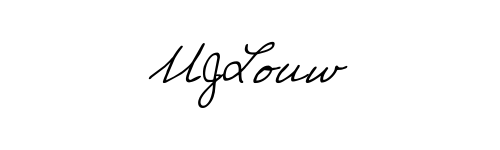
\includegraphics[width = 5cm]{Figures/signature.png} \\
    {Studentenommer / \textit{Student number}} & {Handtekening / \textit{Signature}} \\
    \hline
    UJ Louw & 25/07/2022 \\
    {Voorletters en van / \textit{Initials and surname}} & {Datum / \textit{Date}} \\
    \hline
\end{tabularx}

\vspace{15pt}

% The old declaration

%I, the undersigned, hereby declare that the work contained in this report is my own original work unless otherwise stated.
%
%% Afrikaans:
%% Hiermee verklaar ek, die ondergetekende, dat die werk in hierdie verslag vervat my eie oorspronklike werk is, tensy anders vermeld.
%
%\vspace{2.5cm}
%
%\begin{table}[h]
%\begin{tabular}{@{}p{2.5cm}p{5cm}}
%    Signature: & \dotfill \\
%    & \multicolumn{1}{c}{Obi-Wan Kenobi} \\
%    ~\vspace{1cm} \\
%    Date: & \dotfill \\
%\end{tabular}
%\end{table}
%
%\vfill
%
%\begin{center}
%    Copyright \textcopyright\ 2099 Stellenbosch University \\
%    All rights reserved
%\end{center}


\chapter*{Abstract}
\addcontentsline{toc}{chapter}{Abstract}
\makeatletter\@mkboth{}{Abstract}\makeatother

\subsubsection*{English}

The English abstract.

\selectlanguage{afrikaans}

\subsubsection*{Afrikaans}

Die Afrikaanse uittreksel.

\selectlanguage{english}
\tableofcontents
\listoffigures
\listoftables
\chapter*{Nomenclature\markboth{}{Nomenclature}}
\addcontentsline{toc}{chapter}{Nomenclature}

% \vspace*{-3mm}
\subsubsection*{Variables and functions}

\begingroup
\renewcommand{\arraystretch}{1.2}
\renewcommand{\tabularxcolumn}[1]{p{#1}}
\begin{tabularx}{\textwidth}{@{}p{2.5cm}L}
    $p(x)$ & Probability density function with respect to variable $x$.\\
    $P(A)$ & Probability of event $A$ occurring.\\
    $\varepsilon$ & The Bayes error. \\
    $\varepsilon_u$ & The Bhattacharyya bound. \\
    $B$ & The Bhattacharyya distance. \\
    $s$ & An HMM state.  A subscript is used to refer to a particular state, e.g.\ $s_i$ refers to the $i^{\text{th}}$ state of an HMM. \\
    $\mathbf{S}$ & A set of HMM states. \\
    $\mathbf{F}$ & A set of frames. \\
    $\mathbf{o}_f$ & Observation (feature) vector associated with frame $f$. \\
    $\gamma_s(\mathbf{o}_f)$ & A posteriori probability of the observation vector $\mathbf{o}_f$ being generated by HMM state $s$. \\
    $\mu$ & Statistical mean vector. \\
    $\Sigma$ & Statistical covariance matrix. \\
    $L(\mathbf{S})$ & Log likelihood of the set of HMM states $\mathbf{S}$ generating the training set observation vectors assigned to the states in that set. \\
    $\mathcal{N}(\mathbf{x} | \mu, \Sigma)$ & Multivariate Gaussian PDF with mean $\mu$ and covariance matrix $\Sigma$.\\
    $a_{ij}$ & The probability of a transition from HMM state $s_i$ to state $s_j$. \\
    $N$ & Total number of frames or number of tokens, depending on the context. \\
    $D$ & Number of deletion errors. \\
    $I$ & Number of insertion errors. \\
    $S$ & Number of substitution errors. \\
\end{tabularx}
\endgroup


\newpage
\subsubsection*{Acronyms and abbreviations}

\begingroup
\renewcommand{\arraystretch}{1.2}
\begin{tabular}{@{}p{2.5cm} l}
    AOCS	& Attitude and Orbit Control System \\
    ADCS	& Attitude Determination and Control System \\
    EKF		& Extended Kalman Filter \\
    FDIR	& Fault Detection, Isolation and Recovery \\
    EIC		& Earth Inertial Coordinate \\
    EFC		& Earth Fixed Coordinate \\
    GHA 	& Greenwich Hour Angle \\
    ORC 	& Orbit-referenced Coordinate \\
    SBC 	& Satellite Body Coordinate \\
    DCM 	& Direct Cosine Matrix \\
    TLE 	& Two-line Element \\
    RAAN	& Right Ascension of the Ascending Node \\
    AP		& Argument of Perigee \\
    SGP 	& Simplified General Perturbations \\
    IGRF	& International Geomagnetic Reference Field \\
    IAGA	& International Association of Geomagnetism and Aeronomy \\
    LEO		& Low Earth Orbit \\
    CoM		& Centre of Mass \\
    CoP 	& Centre of Pressure \\
    RW		& Reaction Wheel \\
    FoV		& Field of View \\
    DMD 	& Dynamic Mode Decomposition \\    
    CART	& Classification and Regression Trees \\
    BST		& Binary Searth Tree \\
    LOF		& Local Outlier Factor \\
    IRC		& Inertial-referenced Coordinate \\
    CART	& Classification and Regression Tree \\
    SVM		& Support Vector Machines \\
    RF		& Random Forest \\
    
\end{tabular}
\endgroup

\newpage
\pagenumbering{arabic}

% Contents
%%%%%%%%%%%%%%%%%%%%%%%%%%%%%%%%%%%%%%%%%%%%%%%%
%
% start writing
%
%%%%%%%%%%%%%%%%%%%%%%%%%%%%%%%%%%%%%%%%%%%%%%%%


\chapter{Introduction}
\label{chap:Introduction}
\section{Background}
Since all systems are prone to failure, an engineer's responsibilities involve ensuring that crucial systems are robust to failure and that proper testing and continual maintenance are performed. In the case of satellites, the problem proves even more severe, since most failures are unrecoverable and may lead to mission failure. Satellite systems must therefore be tested thoroughly and be robust to any anomaly. According to \cite{tafazoli2009study}, the attitude determination and control system (ADCS) contributes to the largest percentage of satellite failures as shown in Figure~\ref{fig:OnOrbitFailureSubsystem}. A study conducted by \cite{Jacklin2019} on small satellite mission failures provides a deeper insight into the ADCS's role in satellite failures, since most missions are highly dependent on the ADCS for complete mission success. This is due to many mission specifications that rely on accurate control of the satellite to ensure that payloads, such as cameras, are able to operate as required.

%\begin{figure*}[!htb]
%	\centering
%	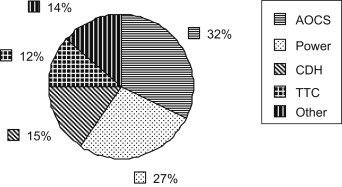
\includegraphics[width = 7cm]{Figures/OnOrbitFailureDistribution.jpg}
%	\caption{On-orbit failure per subsystem \cite{tafazoli2009study}}
%	\label{fig:OnOrbitFailureSubsystem}
%\end{figure*}

%\begin{figure*}[!htb]
%	\centering
%	\begin{tikzpicture}
%	\pie{32/AOCS,
%		27/Power,
%		15/CDH,
%		12/TTC,
%		14/Other}
%	\end{tikzpicture}
%	\caption{On-orbit failures categorised by the subsystem responsible for the mission failure~\cite{tafazoli2009study}.}
%	\label{fig:OnOrbitFailureSubsystem}
%\end{figure*}

The database provided by \cite{swartwout2015cubesat} demonstrates the increase in the number of satellites launched every year. The drastic increase of launched satellites over the past few years further emphasizes this need of ensuring that satellites are robust to failures. Using traditional methods of tracking satellites with ground stations and manually checking for possible failures are therefore not feasible, especially in the case of large satellite constellations. Consequently, most aspects of the satellite need to operate autonomously, especially in the case of attitude control. The focus of this thesis is on a specific aspect of the attitude control which is sensitive to anomalies, namely the attitude determination. 

The extended Kalman filter (EKF) is a sensor fusion algorithm implemented for attitude estimation of the satellite. The objective of this thesis is therefore to develop methods that can be used to avoid unstable and inaccurate estimations from the EKF caused by sensor anomalies.

\section{Problem Description}
For many satellite missions the ADCS is of high importance. It is necessary to effectively control the attitude to fulfill the mission requirements. The control performance is also limited by both the estimation accuracy and performance. A common satellite attitude requirement is to be earth-following during an eclipse, to point the payload to a target and to otherwise point and track the sun for solar charging. Good attitude estimation throughout the entire orbit is necessary to best fulfill these requirements.

The attitude estimation is, however, highly influenced by the sensor readings. Different sensor measurements are fused together, normally with the use of an EKF, to produce a single attitude estimate. If an erroneous, or false measurement is present in the collection of sensors, it will deter and influence the outcome of the fusion algorithm.  Depending on the number of sensors available and the severity of the erroneous sensor, the inluence on the EKF can be reduced estimation accuracy or divergence and instability. It is good practice to develop appropriate tests to protect the EKF against incorrect measurements. 

Anomaly detection in satellite sensors have been investigated in many previous research. The current trend is to use generic sensor anomalies, such as bias drift, high noise, sudden failure or any drastic change in the behavior of the sensor to develop techniques to detect these anomalies. This is only a subset of possible errors and does not assist in diagnosing the anomaly, detecting intermittent errors, or coupled events between sensors. An example of a practical anomaly which can occur and which is difficult to detect using standard techniques are solar reflections from solar panels on a sun sensor. Majority of satellites, even with relatively low attitude requirements, have some form of sun sensor. The sun sensor also provides an accurate measurement during the periods of the orbit where targeting and solar tracking is most likely and where the attitude requirement is the highest. Thus, it would be beneficial to have good interventions to ensure robust sun vector measurements for the EKF.

Since the EKF is also reliant on the mathematical model of the system, the control inputs should also be accurate. Due to actuator failure on satellites, the command control input and the actual control input can differ significantly. This must also be detected and isolated to ensure robust estimation. The satellite must be able to autonomously detect, classify (isolate) and recover from the anomaly to ensure safe operation during orbit. A block diagram for the fault detection, isolation and recovery (FDIR) of the EKF within the ADCS system is provided in Figure~\ref{fig:System_Diagram}. The FDIR is provided with both the inputs from the feature extraction component as well as the sensor measurements to predict whether an anomaly has occurred. Thereafter, the anomaly must be isolated and therefore classified as to which practical anomaly caused the current sensor measurements. The anomaly is then recovered depending on the recovery method and anomaly type.

\begin{figure}[h!b!t]
	\centering
	\def\svgwidth{14cm}
	\import{Figures/}{Control_Diagram.pdf_tex}
	\caption{System Diagram}
	\label{fig:System_Diagram}
\end{figure}

The anomalies discussed and modelled in this thesis are specific to the design of the satellite. The attitude sensors and the anomalies for each sensor is a sun sensor with solar reflection from the solar panels, a infrared-nadir sensor with the moon on the earth's horizon and a magnetometer with magnetic disturbances caused by the magnetic induced dipole moment of the solar panels. The actuator failure is that of a reaction wheel not responding to control inputs. 

\section{Problem Statement}
Practical sensor and actuator anomalies influence the estimation of the EKF that is commonly used in the ADCS of satellites. To ensure that these sensor anomalies can be recovered from, this thesis focusses on different FDIR methods to provide robust estimation of the EKF even with practical sensor and actuator anomalies.

\section{Project Definition}
This project aims to develop and test various methods of detecting sensor anomalies and classifying the anomaly. The anomalies are recovered from in a simulation model wherein practical anomalies are simulated during satellite orbit. The simulation must also be used to create a database of sensor measurements produced by different anomalies. This database provides labelled data for the training of binary and multiclass classification models for detection and isolation, respectively. The trained models should be tested on the simulation environment and the estimation accuracy should be compared between different models and different recovery methods.

This thesis aims to develop an unsupervised learning detection algorithm that is only trained on the normal data and label data samples as anomalies where the relationship between the sensors are considered as an outlier. Although this is the aim of the thesis, supervised learning methods will also be used for detection to provide a comparison between the two groups. Unsupervised learning for detection is desired since it only requires normal data and can detect theoretically detect any anomaly and does not require the anomalous data for training. This means that various anomaly simulations are not required for the detection method.

The isolation, however, requires the labelled data of the multiclass data, since the classification method needs to determine which sensor is faulty. This can therefor not be executed with unsupervised learning methods, unless an unsupervised learning detection model is developed for each individual sensor with the input data being a few timesteps of measurements from that sensor. This however has many complications since the recovery methods should be implemented on every sensor that is anomalous according to the isolation method, and this verges on a cooperative multi-agent problem, which is outside the scope of this thesis. Supervised learning methods are therefore used to classify the sensor that is experiencing the anomaly.

A comparison of the detection accuracy as well as the estimation accuracy of a model in the simulation environment after training on either the generic sensor anomalies or the practical anomalies should also be discussed. A thorough analysis of the each individual component of the FDIR should be conducted and discussed. 

%Fault detection and isolation research for satellites are highly dependent on simulation environments for quick development. However the current trend focuses on general anomalies and not specific modelled anomalies. This therefore produces FDIR systems that are less effective at predicting anomalies and classifying which subsystem or component produces the current anomaly. The focus of this research is to model specific sensor anomalies and develop and analyse prediction models. 
%
%The general sensor anomalies are large noise on sensors or sudden sensor failures. These anomalies are however not based on natural occurrences, but on sensor failures. This thesis focuses on natural occurring anomalies that can produce inaccurate sensor measurements. These anomalies are accurately modelled and recovered by implementing different recovery systems for the Kalman Filter. 

%%% New introduction is written above

%The current trend in industry is to create systems that operate autonomously. There is also a trend seen where multi-agent systems with hundred and thousands of sub-systems work within a larger system. Even though each sub-system can operate independently, the health of the network/system is dependent on each agent within the system operating as desired. Consequently, autonomous systems must be able to detect faults within the system. To attain this, a fault detection, isolation and recovery system is required for each individual agent and the system as a whole.

%\section{Background}
%All systems have the inevitable problem that they will fail. Determining this failure is of a variety of importance for multiple systems. The current tendency is that many systems are more and more integrated. A web of self-driving cars, UAV's for delivery, satellite constellations and more. The problem with any of these systems is if any part of the system is faulty it can have detrimental consequences for a part of the system or the entire system.
%
%Software developers make mistakes, as all humans do. The current industry standard for number of bugs per thousand lines of code is $5$ bugs/KLOC at \$$5$ per line of code. NASA works on 0.004 bugs/KLOC at \$$805$ per line of code. Imagine having hundreds of thousands of lines of code and having that same code on thousands of satellites. Each fault detection must usually be checked with if statements and logic. This leads to more lines of code and mistakes on trying to capture mistakes. I propose a solution to this problem by using statistical models and machine learning to use satellites in close proximity to determine the health of the other nearby components within the system.
%
%\section{Problem description}
%
%https://www.theverge.com/2020/1/14/21043229/spacex-starlink-satellite-mega-constellation-concerns-astronomy-space-traffic
%
%The most detrimental effect could be on satellite constellations. Satellites are expensive, \$$500 000$ each for Starlink satellite. And this is also based on the mass production of satellites. Satellites cannot merely be accessed and fixed as other systems. Therefore satellites are used as the specific system for FDIR of systems.
%
%The current situation with CubeSats is that ground stations will not be able to keep up with the fault detection and diagnosis of CubeSats within constellations where thousands of CubeSats are within the same height above the earth. As is the current situation with Starlink.
%
%Kessler syndrome is the effect of one satellite, that is unable to control its orientation and position, causing a collision in orbit. This leads to more debris in the orbit and more collisions and this is detrimental if considered in view of Starlink's mega-constellation.
%
%\section{Research hypothesis}
%I propose a fault detection system for each individual satellite and the constellation as a whole. The satellite will have an on-board FDIR system that also uses the information of the satellites closest to its position to provide feedback of its own "health" and the health of the other satellites in its orbit. If a satellite is determined "unhealthy" by all the nearby satellites then the satellite with go into safe mode until the ground station can determine the problem with current satellite.
%
%\section{Scope and objectives}
%
%The following objectives will be pursued in this project/thesis/dissertation:
%\begin{enumerate}[label=\Roman*]										% \usepackage{enumitem}
% \item To \textit{conduct} a thorough survey of the literature related to:
% \begin{enumerate}[label=(\alph*)]
%  \item facility location problems in general,
%  \item models for the placement of a network of radio transmitters in particular,
%  \item the nature of parameters required to describe effective radio transmission, and
%  \item terrain elevation data required to generate an instance of the bi-objective radio transmitter location problem described in the previous section.
% \end{enumerate}
% \item  To \textit{establish} an suitable framework for evaluating the effectiveness of a given set of placement locations for a network of radio transmitters in respect of its total area coverage and its mutual area coverage.
% \item To \textit{formulate} a bi-objective facility location model suitable as a basis for decision support in respect of the location of a network of radio transmitters with a view to identify high-quality trade-offs between maximising total coverage area and maximising mutual coverage area.  The model should take as input the parameters and data identified in Objective~I(c)--(d) and function within the context of the framework of Objective~II.
% \item To \textit{design} a generic \textit{decision support system} (DSS) capable of suggesting high-quality trade-off locations for user-specified instances of the bi-objective radio transmitter location problem described in the previous section.  This DSS should incorporate the location model of Objective~III.
% \item To \textit{implement} a concept demonstrator of the DSS of Objective IV in an applicable software platform.  This DSS should be flexible in the sense of being able to take as input an instance of the bi-objective radio transmitter location problem described in the previous section via user-specification of the parameters and data of Objectives I(c)--(d) and produce as output a set of high-quality trade-off transmitter locations for that instance.
% \item To \textit{verify} and validate the implementation of Objective V according to generally accepted modelling guidelines.
% \item To \textit{apply} the concept demonstrator of Objective V to a special case study involving realistic radio transmission parameters and real elevation data for a specified portion of terrain.
% \item To \textit{evaluate} the effectiveness of the DSS and associated concept demonstrator of Objectives~IV--VI in terms of its capability to identify a set of high-quality trade-off solutions for a network of radio transmitter locations.
% \item To \textit{recommend} sensible follow-up work related to the work in this project which may be pursued in future.
%\end{enumerate}

%\section{Research methodology}
%\blindtext

\section{Thesis Outline}
Chapter~\ref{chap:Introduction} provides the background and motivation for this research as well as the project definition and thesis outline.
\\
Chapter~\ref{chap:Literature Study} discusses the relevant research that has been done on FDIR.
\\
Chapter~\ref{chap:SatDesign} described the satellite design used for the simulation environment as well as the modelling of the sensor anomalies.
\\
Chapter~\ref{chap:Simulation} demonstrates the development and implementation of the simulation environment as shown in Figure~\ref{fig:System_Diagram}.
%\\
%Chapter~\ref{chap:ADCS} discusses the satellite design and expands on the elements $\mathbf{D}_k$, $\mathbf{S}_k$, $\mathbf{E}_k$ and $\mathbf{W}_k$ in Figure~\ref{fig:System_Diagram}.
\\
Chapter~\ref{chap:Anomalies} provides the mathematical models of the specific anomalies and the effects thereof on the satellite.
\\
Chapter~\ref{chap:Feature Extraction} describes the feature extraction methods used in this thesis to enhance the accuracy of the detection and classification models, also provided as a element in Figure~\ref{fig:System_Diagram}.
\\
Chapter~\ref{chap:Recovery} provides various recovery methods and demonstrates the theoretical possibility of the methods based on perfect prediction accuracy.
\\
Chapter~\ref{chap:Detection} describes the different algorithms and methods used to detect an anomaly in the system.
\\
Chapter~\ref{chap:Isolation} describes the different algorithms and methods used to classify an anomaly in the system.
\\
Chapter~\ref{chap:Results} provides a summary of all the results for the combination of best methods as provided in Chapter~\ref{chap:Feature Extraction}, Chapter~\ref{chap:Recovery}, Chapter~\ref{chap:Detection} and Chapter~\ref{chap:Isolation}.
\\
Chapter~\ref{chap:Conclusion} discusses the influence of modelling specific anomalies on the prediction accuracy and robustness of a EKF.
\chapter{Literature Study}
\label{chap:Literature Study}

The implementation of FDIR on satellites have multiple complications with regards to the type of data generated by a satellite and the methodologies that can be implemented within the time and memory constraint of a cube-sat processor.

%\section{Strategies for Satellite Constellations}
%\cite{Castel2006}
%
%\subsection{Individual Strategy}
%Each satellite performs it's own FDIR without communication with other satellites. Consequently, the satellite has its own algorithms and knowledge of when a fault occurs within it's own system and is only required to communicate with the ground station.
%
%\subsection{Centralised Strategies}
%Centralised strategies focus on the FDIR of the entire constellation performed by a single entity. This can either be one of the satellites or the ground station.
%\subsubsection{Master Centralised Strategy}
%
%\subsubsection{Opportunistic Centralised Strategy}
%
%\subsubsection{Global Centralised Strategy}
%
%\subsection{Mixed Strategy}
%
%\subsection{Distributed Strategies}
%\subsubsection{Common Distributed Strategy}
%
%\subsubsection{Individual Distributed Strategy}

\section{Anomaly Detection on Satellites}
Various methodologies have been tested on different component of satellites. Therefore a summary of these research articles are provided in this section.

\subsection{Analysis and Prediction of Satellite Anomalies}
%\cite{Wintoft}

\subsection{Agent-based algorithm for fault detection and recovery of gyroscope's drift in small satellite missions}
To ensure that the ADCS of satellites are autonomous every aspect of the control must be able to recover from faults. \cite{carvajal2017agent} developed an algorithm to evaluate the control of a gyroscope and detect whether drifting exists. If drifting is detected another algorithm is deployed to ensure the recovery of the gyroscope drift by updating the error state vector.

\textbf{Multivariate Anomaly Detection in Discrete and Continuous Telemetry Signals Using a Sparse Decomposition in a Dictionary}
\cite{Pilastre2020}

\textbf{Fault isolation of reaction wheels onboard three-axis controlled in-orbit satellite using ensemble machine learning}
\cite{rahimi2020fault}

\textbf{Fault tolerant control for satellites with four reaction wheels}
\cite{jin2008fault}

\textbf{Innovative Fault Detection, Isolation and Recovery Strategies On-Board Spacecraft: State of the Art and Research Challenges}
\cite{wander2013innovative}

\textbf{Machine learning methods for spacecraft telemetry mining}
\cite{ibrahim2018machine}

\textbf{Machine learning techniques for satellite fault diagnosis}
\cite{ibrahim2020machine}

\textbf{Satellite fault diagnosis using a bank of interacting Kalman filters}
\cite{Tudoroiu2007}

\textbf{A scheme of satellite multi-sensor fault-tolerant attitude estimation}
\cite{Zhou2016} implements a fault tolerant federated Kalman filter with three sub-filters for multi-sensor fault estimation. 

\textbf{Detection of satellite attitude sensor faults using the UKF}
\cite{Xiong2007} provides a fault detection method by using the residuals generated by an unscented Kalman filter to detect anomalies with a threshold based on a confidence level. 


\textbf{Sensor fault detection and recovery in satellite attitude control}
\cite{Nasrolahi2018} 

\textbf{Sensor Failure Detection in Dynamical Systems by Kalman Filtering Methodology}
While methods for sensor failure detection in other dynamical systems has also been developed which includes kalman filter methodology~\cite{Ciftciogl1991},

\textbf{Sensors Anomaly Detection of Industrial Internet of Things Based on Isolated Forest Algorithm and Data Compression}
isolation forests~\cite{Liu2021} and using LSTM on sensor data to detect anomalies on machines 

\textbf{LSTM-based Encoder-Decoder for Multi-sensor Anomaly Detection}
\cite{Malhotra2016}

\textbf{Sensor fault detection and isolation using adaptive extended Kalman filter}
\cite{van2012sensor}

\section{Statistical Methods}
\subsection{Pearson Correlation}
Vectors of certain sensors are highly correlated. For instance the vector of the earth sensor is highly correlated since the magnitude of the vector remains more or less constant. To detect anomalies the correlation of vectors can be measured and with a specified threshold the correlation can be indicated as a anomaly or nor.

The squared Pearson correlation coefficient (SPCC) for vectors depicted as
\linebreak
\\
\centerline{$a = [a_1, a_2, \ldots, a_L]^T,$}
\linebreak
\centerline{$b = [b_1, b_2, \ldots, b_L]^T,$}
\\
is defined as \cite{benesty2009pearson}
\begin{equation}
	\rho^2 (a,b) = \frac{E^2 (a,b)}{E(a^Ta)E(b^Tb)}.
\end{equation}
The correlation coefficient is proven to be constraint as
\begin{equation}
	0 \leq \rho \leq 1,
\end{equation}
where $\rho = 1$ is perfect linear correlation. 

\subsection{Variance}
Within a sequential data sample of the satellite, the variance of the variables should be within a given threshold if the satellite is in a stable condition. The variance of the data sample is defined as 
\begin{equation}
	S^2 = \frac{\sum(x_i + \bar{x})^2}{n-1}
\end{equation}
where $x$ defines the variable within the dataset.

\subsection{Kalman-Filter}
The Kalman-filter application would require the state-space matrices to be provided in the log file.

\subsection{Multivariate Guassian Distribution}
The assumption that the error of our data is generated with a Guassian distribution with a specific mean, $\mu$, and variance, $\sigma^2$, provides the opportunity for using multi-variate Gaussian distribution to determine the probability of a data-sample within a dataset. 
\begin{equation}
	\label{mean}
	\mu_j = \frac{1}{m} \sum_{i=1}^{m}x_j^{(i)}
\end{equation}

\begin{equation}
	\label{variance}
	\sigma_j^2 = \frac{1}{m} \sum_{i=1}^{m}(x_j^{(i)} - \mu_j)^2
\end{equation}

\begin{equation}
	\label{guassian distribution}
	p(x) = \prod_{j=1}^{n} \frac{1}{\sqrt{2\pi}\sigma_j}exp(-\frac{(x_j-\mu_j)^2}{2\sigma_j^2})
\end{equation}

For multi-variate Guassian distribution \cite{do2008multivariate}.

\begin{equation}
	\label{sum}
	\sum = \frac{1}{m}\sum_{i=1}^{m}(x^{(i)}-\mu)(x^{(i)}-\mu)^T
\end{equation}

\begin{equation}
	\label{multi-variate guassian distribution}
	p(x) = \frac{1}{(2\pi)^{\frac{n}{2}}{\lvert \sum \rvert}^\frac{1}{2}} exp(-\frac{1}{2}(x-\mu)^T{\sum}^{-1}(x-\mu))
\end{equation}

The Anomalies will be classified based on probabilities smaller than a given threshold $p(x) < \epsilon$.

\begin{algorithm}[!htb]
	\caption[Multi-variate Guassian Distribution]{Multi-variate Guassian Distribution Algorithm}
	\label{alg}
	\begin{algorithmic}[1]
		\State Determine feature vectors $x_i$
		\State Determine threshold probabilty, $\epsilon$
		\State Calculate $\mu_j$ with Eq~\ref{mean}
		\State Calculate $\sigma_j$ with Eq~\ref{variance}
		\State Calculate $p(x)$ with Eq~\ref{guassian distribution}
		\If{$p(x) < \epsilon$}
			\State Anomaly $= True$
		\Else
			\State Anomaly $= False$
		\EndIf
		
	\end{algorithmic}
\end{algorithm}

\subsection{Kullback-Leibler Divergence}
The Kullback-Leibler divergence quantifies the difference between two probability density functions, denoted as $p(x)$ and $q(x)$ \cite{hershey2007approximating}. Satellites are systems that are predictable within a time-series. The divergence between two sequential data buffers from the satellite will have a very similar probability distribution. Therefore calculating the difference between two datasets can be used to detect an anomaly based on a given threshold.

The difference between the probability distributions from datasets, $a$ and $b$, in Figure~\ref{Guassian plot} cannot simply be calculated as the difference in the mean or the difference in the variance. To overcome this, the divergence between the two distributions can be calculated. Intuitively a point $x$ with a high probability in the dataset $a$ should have a high probability in the dataset $b$ if the two datasets have a small divergence. 

\pgfmathdeclarefunction{gauss}{3}{%
	\pgfmathparse{1/(#3*sqrt(2*pi))*exp(-((#1-#2)^2)/(2*#3^2))}%
}
\begin{figure}[!h]
	\centering
	\textbf{Difference Between Probability Distributions}
	\begin{tikzpicture}
		\begin{axis}[
			no markers, 
			domain=-3:6, 
			samples=100,
			ymin=0,
			axis lines*=left, 
			xlabel=$x$,
			every axis y label/.style={at=(current axis.above origin),anchor=south},
			every axis x label/.style={at=(current axis.right of origin),anchor=west},
			height=5cm, 
			width=12cm,
			xtick=\empty, 
			ytick=\empty,
			enlargelimits=false, 
			clip=false, 
			axis on top,
			grid = major,
			hide y axis
			]
			
			\addplot [very thick,cyan!50!black] {gauss(x, 3, 1)};
			
			\pgfmathsetmacro\valueA{gauss(3,3,1)}
			\draw [gray] (axis cs:3,0) -- (axis cs:3,\valueA);
			
			\node[below] at (axis cs:3, 0)  {$\mu_p$}; 
			
			\addplot [very thick,red!50!black] {gauss(x, 1.5, 1.5)};
			
			\pgfmathsetmacro\valueB{gauss(1.5,1.5,1.5)}
			\draw [gray] (axis cs:1.5,0) -- (axis cs:1.5,\valueB);
			
			\node[below] at (axis cs:1.5, 0)  {$\mu_q$}; 
		\end{axis}
		
	\end{tikzpicture}
	\caption{Guassian Distributions}
	\label{Guassian plot}
\end{figure}

The divergence can be expressed as 

\begin{equation}
	KL(P\lvert\lvert Q) = \int p(x) \log \left( \frac{q(x)}{p(x)} \right)dx.
\end{equation}

\subsection{Canonical Correlation Analysis}
Due to the orbital nature of satellites there exist a correlation between various sensors. For instance the sun sensor, magnetometer and earth sensor are correlated based on the desired orientation and orbit of the satellite. This correlation might not be of linear nature, but with non-linear correlation methods such as kernel canonical correlation the correlation can be measured.

However, canonical correlation provides the measure of correlation between a multi-dimensional variable with another multi-dimensional variable. Although this seems profitable for satellite fault detection, it will only be applicable for each the comparison between individual sensors. This will indicate the non-linear correlation of the sun sensor with regards to the magnetometer. The problem however, according to \cite{chen2017fault} is to, determine the appropriate threshold for which to classify a fault. \cite{chen2017fault} proposed a method for determining the appropriate threshold on page 5, algorithm 1.
\cite{fukumizu2007statistical}
\cite{zhu2017quality}

Python - Pyrcca package

\subsubsection{K-means-based}
\subsubsection{Guassian Mixture Model}
\subsubsection{Just-In-Time-Learning}
\cite{chen2020just}

\section{Feature Extraction}
To 
https://towardsdatascience.com/feature-extraction-techniques-d619b56e31be
\subsection{Prony's Method}
\subsection{Convolutional Networks}
\subsection{K-means Clustering}
K-clustering: Clustering multiple points with similar features.
%\subsection{Principal Component Analysis}
%\cite{choi2005fault}
%\cite{ding2010application}
\subsection{Partial Least Square}
%\subsection{Independent Component Analysis}
\subsection{Locally Linear Embedding}
%\subsection{Linear Discriminant Analysis}
%\subsection{Autoencoder}
\subsection{t-Distributed Stochastic Neighbor Embedding}


\section{Supervised Learning}
Supervised learning consists of models that are trained on labelled data. This is not a problem with simulation, but with the real data, it is a problem and to provide tests on the real data to label it must be proficient. If unsupervised learning and statistical methods are not sufficient in their accuracy, a method for labelling the real data must be provided.

\subsection{Decision Trees}
For decision trees in the use of classification we use the Gini score

\begin{equation}
	G = \sum_{k=1}^{K} \hat{p}_{k} (1-\hat{p}_{k})
\end{equation}

\subsection{Random Forests}
\cite{Shi2006, Paul2018, Primartha2018}

\subsection{Long Short Term Memory}
Time-series data: LSTM or DLSTM

\subsection{Support Vector Machines}
Support Vector Machines

\subsection{Naive Bayes}
Naive Bayes

\subsection{K-nearest neighbours}
K-nearest neighbours

\subsection{Artificial Neural Networks}
Artificial Neural Networks

\section{Unsupervised Learning}
Density-based, distance, Clustering

\subsection{Kernel Adaptive Density-based}
Kernel adaptive density-based: Is an algorithm that uses the density factor of a data point relative to other data points to determine whether the data point is an outlier or not.

\subsection{Loda}
Loda: Is a fast and efficient anomaly detection algorithm that used histograms to evaluate data points to determine whether a data point is an outlier. Loda is an on-line method and not a batch method.

\subsection{Robust-kernel Density Estimation}
Robust-kernel density estimation

\section{Reinforcement Learning}
Active Anomaly detection with meta-policy (Meta-AAD) is a deep reinforcement learning approach that is based on the actor-critic model. The agent must query data points within the given dataset (where the queried point is the data top 1 data point). The query is given to a human 

\section{Summary}


\chapter{Simulation}
\label{chap:Simulation}

To implement and research various FDIR systems on satellites a simulation of satellite dynamics and kinematics is developed. The focus of this thesis is on small satellites and more specifically CubeSats. For the simulation of the ADCS of the satellite \cite{auret2012design, JansevanVuuren2015, Jordaan2016} were referenced during the development of the satellite simulation. The simulation was developed in Python to simulate the dynamics and kinematics during a satellite orbit. \textbf{TODO: Decide whether satellite design should be within this chapter}.

\section{Attitude Determination and Control System}

For the mission of the specific satellite in this document the main operational goal of the ADCS on this specific satellite mission is to control the payload to point towards the centre of the Earth during eclipse and point the solar panels towards the sun during the sunlit phase. To ensure this is accurately simulated the different coordinate frames dominating a satellite orbit, the attitude of the satellite as well as the satellite dynamics and kinematics is discussed in this section.

\subsection{Coordinate Frames}
The coordinate frames in aerospace is a fundamental part of the ADCS. To determine the orientation and position of an object, it should be relative to a fixed frame. Consequently, the Earth inertial coordinate (EIC) frame, $\mathcal{E}\{\bar{\mathbf{x}}_{\mathcal{E}},~\bar{\mathbf{y}}_{\mathcal{E}},~\bar{\mathbf{z}}_{\mathcal{E}}\}$, is the fixed frame from which every other frame is relative to.

A coordinate frame consists of three orthogonal vectors which is commonly referred to as x, y, and z. The axis of the coordinate frame is appropriately named as the X-axis, Y-axis and Z-axis. A vector ($\mathbf{r}$) within the coordinate frame can thus be expressed as 
\begin{equation}
\mathbf{r} = x\mathbf{i} + y\mathbf{j} + z\mathbf{k}
\end{equation}
where the magnitude of $\mathbf{r}$ is denoted as $\norm{\mathbf{r}}$ and is equal to 
\begin{equation}
\norm{\mathbf{r}} = \sqrt{x^2 + y^2 + z^2}.
\end{equation}

The Earth-centered coordinate frames are dived into two, namely the EIC and Earth fixed coordinate (EFC) frame, $\mathcal{F}\{\bar{\mathbf{x}}_{\mathcal{F}},~\bar{\mathbf{y}}_{\mathcal{F}},~\bar{\mathbf{z}}_{\mathcal{F}}\}$. EFC is fixed to the Earth and rotates with it, while EIC is inertial fixed.

% Insert a figure of the Earth coordinate frames here

The EIC is defined as the Z-axis pointing towards the north pole, the X-axis pointing towards the Vernal Equinox, $\Upsilon$, and the Y-axis completing the orthogonal set. The EFC is a copy of the EIC, with the Z-axis being identical, however the EFC rotates with the Earth. The EFC in relation to the EIC can be expressed by a single angle of rotation, which is the Greenwich Hour Angle (GHA), $\alpha_G$. With the elapsed time, $t$, since $t_0$, the angular rate of the Earth, $\omega_E$, and the GHA, $\alpha_{G,0}$, at $t = t_0$, $\alpha_G$ can be calculated as 
\begin{equation}
\alpha_G = \omega_Et + \alpha_{G,0}.
\end{equation}
To transform a vector from one coordinate frame to another, a transformation matrix, $\boldsymbol{A}$, is required. For example vector $\mathbf{r}_{\mathcal{F}}$ can be transformed to $\mathbf{r}_{\mathcal{E}}$ with 
\begin{equation}
\mathbf{r}_{\mathcal{E}} = \boldsymbol{A}^{\mathcal{E}}_{\mathcal{F}}\mathbf{r}_{\mathcal{F}}
\end{equation}
with $\boldsymbol{A}^{\mathcal{E}}_{\mathcal{F}}$ being the EFC-to-EIC transformation matrix. Due to the definition of both coordinate frames, $\boldsymbol{A}^{\mathcal{E}}_{\mathcal{F}}$ can be defined as

\begin{equation}
\boldsymbol{A}^{\mathcal{E}}_{\mathcal{F}} = 
\begin{bmatrix}
	\text{cos}(\alpha_G) & -\text{sin}(\alpha_G) & 0\\
	\text{sin}(\alpha_G) & \text{cos}(\alpha_G) & 0 \\
	0 & 0 & 1
\end{bmatrix}.
\end{equation}
To determine the satellite position, satellite-centred coordinate frames must be used. Three satellite-centred coordinate frames are used, namely the inertial-reference coordinate frame (IRC), $\mathcal{I}\{\bar{\mathbf{x}}_{\mathcal{I}},~\bar{\mathbf{y}}_{\mathcal{I}},~\bar{\mathbf{z}}_{\mathcal{I}}\}$,  which remains inertial fixed, the orbit-referenced coordinate (ORC) frame, $\mathcal{O}\{\bar{\mathbf{x}}_{\mathcal{O}},~\bar{\mathbf{y}}_{\mathcal{O}},~\bar{\mathbf{z}}_{\mathcal{O}}\}$ and the satellite body coordinate (SBC) frame, $\mathcal{B}\{\bar{\mathbf{x}}_{\mathcal{B}},~\bar{\mathbf{y}}_{\mathcal{B}},~\bar{\mathbf{z}}_{\mathcal{B}}\}$. 
% The IRC frame is only acknowledged, since it is the frame that is fixed (as it does not rotate around the centre of the satellite), however it changes position with the orbit of the satellite. This frame is not used to determine the position of the satellite and will not be referenced for the remainder of this document.

The ORC frame changes location as the satellite moves, however the Z-axis is always pointing towards the centre of the Earth, with the Y-axis being the orbit anti-normal and the X-axis completing the orthogonal set. To transform a vector from the EIC frame to the ORC frame the unit position vector, $\mathbf{r}_{sat}$ and the unit velocity vector, $\mathbf{v}_{sat}$ in EIC is required \cite{Chen_ground-target}. The EIC to ORC transformation matrix, $\boldsymbol{A}^{\mathcal{O}}_{\mathcal{E}}$, is calculate as
\begin{equation}
\label{Eq: ORC to EIC}
\begin{aligned}
	\boldsymbol{A}^{\mathcal{O}}_{\mathcal{E}} &= 
	\begin{bmatrix}
		\mathbf{u} & \mathbf{v} & \mathbf{w}\\
	\end{bmatrix}^T \\
\text{where} \quad
\mathbf{w} &= -\frac{\mathbf{r}_{sat}}{\norm{\mathbf{r}_{sat}}} \\
\mathbf{v} &= -\frac{\mathbf{r}_{sat} \times \mathbf{v}_{sat}}{\norm{\mathbf{r}_{sat} \times \mathbf{v}_{sat}}} \\
\mathbf{u} &= \mathbf{v} \times \mathbf{w}. \\
\end{aligned}
\end{equation}

The SBC frame is the frame fixed to the satellite and it is the relative rotation of the satellite in relation to the ORC. Thus for the mission of this satellite it is required that the SBC and ORC frames coincide during eclipse. For the transformation of a vector from the ORC to SBC frame, the direct cosine matrix (DCM) also referred to as $\boldsymbol{A}$ or $\boldsymbol{A}^{\mathcal{B}}_{\mathcal{O}}$ is used. For the remainder of the document the DCM will be referred to as $\boldsymbol{A}^{\mathcal{B}}_{\mathcal{O}}$ to avoid any confusion. The calculation of this transformation matrix is discussed in $\S$\ref{subsection_quaternions} and implemented with Eq~\ref{eq:DCM_quaternion}.

% Insert a figure of the satellite coordinate frames here

\subsection{Attitude}
\label{subsection_quaternions}
To determine the attitude of an object, a model must be used to determine the rotation of an object in three dimensions. For this the visual and intuitive example of the Euler angles exist. Euler angles are the rotation of an object around three orthogonal axis, that change orientation with the rotation of the object. The three axes, denoted by $x$, $y$ and $z$ rotate with the object as depicted in Figure~\ref{fig:Pitch}.
\begin{figure}[!htb]
	\centering
	\def\svgwidth{10cm}
	\import{Figures/}{Pitch.pdf_tex}
	\caption{Euler angles}
	\label{fig:Pitch}
\end{figure}

$\boldsymbol{A}^{\mathcal{B}}_{\mathcal{O}}$ can be used to calculate the attitude transformation from given Euler angle rotations. This is done by multiplying the transformation matrices representing each individual Euler angle rotation. The $\boldsymbol{A}^{\mathcal{B}}_{\mathcal{O}}$ can therefore be calculated as 
\begin{equation}
	\begin{aligned}
		\boldsymbol{A}^{\mathcal{B}}_{\mathcal{O}} &= \boldsymbol{A}_{\psi} \boldsymbol{A}_{\phi} \boldsymbol{A}_{\theta} \\
			&= \begin{bmatrix}
			\text{cos} \psi & \text{sin} \psi & 0 \\
			-\text{sin} \psi & \text{cos} \psi & 0 \\
			0 & 0 & 1
			\end{bmatrix} \begin{bmatrix}
			1 & 0 & 0 \\
			0 & \text{cos} \phi & \text{sin} \phi \\
			0 & -\text{sin} \phi & \text{cos} \phi
			\end{bmatrix} \begin{bmatrix}
			\text{cos} \theta &  0 & -\text{sin} \theta \\
			0 & 1 & 0 \\
			\text{sin} \theta & 0 & \text{cos} \theta
			\end{bmatrix}. \\
	\end{aligned}
\end{equation}
Euler angles however are not always a suitable method in determining the attitude of a satellite. This is because of singularities that can occur such as the gimbal-lock effect. Where two rotational axis, coincide to form a single rotational axis. Consequently, not all $3$D rotations can be described with Euler angles, because with gimbal-lock only two effective rotations can occur instead of three \cite{diebel2006representing}. Therefore the method of describing $3$D rotation with quaternions is more often used and more convenient. 

A quaternion, $\mathbf{q}$, has four components that are dependent on one another and constrained by 
\begin{equation} 
\label{Eq-quaternion dependency}
q_1^2 + q_2^2 + q_3^2 + q_4^2 = 1.
\end{equation}
The attitude quaternion is also related to the Euler angles in that if the Euler rotational axis from ORC to SBC is defined as a unit vector $\mathbf{e} = \begin{bmatrix} e_1  & e_2 & e_3 \end{bmatrix}^T$ and the angle of the Euler rotation is $\Phi$ then $\mathbf{q}$ can be expressed as
\begin{equation}
\mathbf{q} = \begin{bmatrix} e_1 \text{sin}(\frac{\Phi}{2}) \\ e_2 \text{sin}(\frac{\Phi}{2}) \\ e_3 \text{sin}(\frac{\Phi}{2}) \\ \text{cos}(\frac{\Phi}{2}) \end{bmatrix}
\end{equation}
It is difficult to visualize a quaternion, however the most simplistic method of understanding it is shown in Figure~\ref{fig:quaternion}. A quaternion is consequently a unit vector protruding from the centre point of an object as well as the angle of rotation of that object around that unit vector. As seen in Figure~\ref{fig:Pitch} the angle $\theta$ is the angle of rotation around the $z$-axis, for quaternions the angle of rotation is the same principle, however the axis around which the object is rotating, is the unit vector. Therefore, $q_4$ provides the angle of rotation while, $q_{1-3}$ represents the unit vector, however with the condition of Eq~\ref{Eq-quaternion dependency}.

\begin{figure}[!htb]
	\centering
	\def\svgwidth{10cm}
	\import{Figures/}{quaternion.pdf_tex}
	\caption{Graphical quaternion representation}
	\label{fig:quaternion}
\end{figure}

$\boldsymbol{A}^{\mathcal{B}}_{\mathcal{O}}$ can also be transformed as a function of $\mathbf{q}$ \cite{wertz2012spacecraft} through

\begin{equation}
\label{eq:DCM_quaternion}
	\boldsymbol{A}^{\mathcal{B}}_{\mathcal{O}}
		= \begin{bmatrix}
		q_1^2 - q_2^2 - q_3^2 + q_4^2 & 2(q_1q_2 + q_3q_4) & 2(q_1q_3 - q_2q_4) \\
		2(q_1q_2 - q_3q_4) & -q_1^2 + q_2^2 - q_3^2 + q_4^2 & 2(q_2q_3 + q_1q_4) \\
		2(q_1q_3 + q_2q_4) & 2(q_2q_3 - q_1q_4) & -q_1^2 - q_2^2 + q_3^2 + q_4^2 \\
		\end{bmatrix}.
\end{equation}
The quaternion is used for attitude determination and therefore also for the attitude control. A error between the commanded quaternion, $\mathbf{q}_c$ and the current quaternion, $\mathbf{q}$, is required for proportional control. This is discussed in section~\ref{section: Quaternion Feedback Controller}.

\subsection{Satellite Kinematics and Dynamics}
The conservation of momentum dominates the dynamics of a satellite. This consists of the torques applied to the satellite, and are mainly control torques, $\mathbf{N_c}$, or disturbance torques, $\mathbf{N_d}$, as well as the moment of inertia of the satellite, $\mathbf{I}$, multiplied by the inertial-referenced angular acceleration of the satellite, $\boldsymbol{\dot{\omega}}_{\mathcal{B}}^{\mathcal{I}}$. The control torques used in this design are only reaction wheel torques, $\mathbf{N}_w$, and magnetorquer torques, $\mathbf{N}_m$. The disturbance torques are discussed in detail in section~\ref{section: disturbance models}, therefore it can only be mentioned that the disturbance torques are the gravity gradient torque, $\mathbf{N}_{gg}$, the wheel imbalance torque, $\mathbf{N}_{rw}$, the gyroscopic coupling torque, $\mathbf{N}_{gyro}$, and the aerodynamic disturbance torque, $\mathbf{N}_{aero}$. The Euler dynamic equation can therefore be given as

\begin{equation}
\begin{aligned}
	\mathbf{J}\boldsymbol{\dot{\omega}}_{\mathcal{B}}^{\mathcal{I}} &= \mathbf{N_c} + \mathbf{N_d}, \\
	\text{where} \quad \mathbf{N_d} &\approx \mathbf{N}_{aero} - \mathbf{N}_{gyro} + \mathbf{N}_{gg} + \mathbf{N}_{rw}, \\
	\text{and} \quad \mathbf{N_c} &= \mathbf{N}_{m} - \mathbf{N}_{w}.
\end{aligned}
\label{Eq-EulerDynamic}
\end{equation}

This is the overarching equation that will be used to determine the control torque as well as the model update of the extended Kalman Filter (EKF). The integration method used in the simulation is the $4^{th}$ order Runge-Kutta method to solve the differential equations. This is demonstrated with Algorithm~\ref{alg: runge-kutta}.

\begin{algorithm}[!htb]
	\caption[$4^{th}$ order Runge-Kutta]{$4^{th}$ order Runge-Kutta}
	\label{alg: runge-kutta}
	\begin{algorithmic}[1]
		\State Definitions: Ts - Timestamp; 
		\State $h = Ts/I$ 
		\For{$n \coloneqq 1$ \textbf{to} $I$}
		\State	$k_1 = hf(x_n, y_n)$
		\State	$k_2 = hf(x_n + \frac{h}{2}, y_n + \frac{k_1}{2})$
		\State	$k_3 = hf(x_n + \frac{h}{2}, y_n + \frac{k_2}{2})$
		\State	$k_4 = hf(x_n + h, y_n + k_3)$
		\State	$y_{n+1}=y_n + \frac{k_1}{6} + \frac{k_2}{3} + \frac{k_3}{3} + \frac{k_4}{6}$
		\EndFor

	\end{algorithmic}
\end{algorithm}

Where $h$ is the step size, which is set to $T_s/10$, and the time step, $T_s$, is equal to one second. $f(x_n, y_n)$ is the Euler dynamic function and Algorithm~\ref{alg: runge-kutta} is used to calculate $\boldsymbol{\omega}_{\mathcal{B}}^{\mathcal{I}}$.  With this procedure the dynamics and kinematics of the satellite can be simulated after each time step.

\section{Environment}
To ensure an accurate simulation environment certain aerospace phenomena must be simulated to ensure that all anomalies can be accurately modelled as well as creating an accurate representation of the satellite orbit. Therefore, the position of the satellite with respect to the Earth (orbit propagation) is required to determine most of the elementary principles of the satellite mission. The orbit propagation is further used to determine the moon on the Earth horizon anomaly. The sun position is required for eclipse as well as simulating the sun reflecting from the solar panels unto the sun sensor. The magnetic field is required to simulate $\mathbf{N}_m$ of the magnetorquer as well as the solar panel dipole anomaly and disturbance torque. \textbf{TODO: Consider a section on CubeSat design}.

\subsection{Orbit Propagation}
The satellite position, $\mathbf{r}_{sat}$ and velocity $\mathbf{v}_{sat}$ at a given time step is required to determine the multiple different variables required for the simulation environment. Therefore the refined version and fourth generation of the simplified general perturbations (SGP) model, namely SGP4, is used as orbit propagator of the satellite after each time step \cite{vallado2006revisiting}. 

To determine $\mathbf{r}_{sat_k}$ and $\mathbf{v}_{sat_k}$ at time step, $k$, the two-line element, (TLE), set of the satellite is required. The TLE set is an encoding of the specified satellite orbit, that requires parameters such as the semimajor axis, $a$, right ascension of the ascending node (RAAN), $\Omega$, argument of perigee (AP), $\omega$, inclination, $i$, eccentricity, $e$, and the time at the beginning of the orbit as a Julian date, $J_t$. With these parameters and the elapsed time since $J_t$, both $\mathbf{r}_{sat_k}$ and $\mathbf{v}_{sat_k}$ can be determined from the World Geodetic System 72 constants that is implemented through the SGP4 model. An example of the satellite orbit propagated by the SGP4 model is illustrated in Figure~\ref{fig:EarthOrbit}.

\begin{figure}[!htb]
	\centering
	\def\svgwidth{10cm}
	\import{Figures/}{EarthOrbit.pdf_tex}
	\caption{SGP4 orbit propagation}
	\label{fig:EarthOrbit}
\end{figure}


The SGP4 outputs the $\mathbf{r}_{sat_k}$ and $\mathbf{v}_{sat_k}$ in the EIC reference frame. The SGP4 is implemented with the SGP4 python package~\cite{sgp4}. Therefore, with $\mathbf{r}_{sat_k}$ and $\mathbf{v}_{sat_k}$ known, $\boldsymbol{A}^{\mathcal{O}}_{\mathcal{E}}$ can now be calculated according to Eq~\ref{Eq: ORC to EIC}.

\subsection{Sun}
For the mission to be successful it is critical to determine the position of the sun relative to the satellite. This is because the satellite must determine whether it is in the eclipse to determine the control operation. Therefore, the model from \cite{vallado2001fundamentals} is implemented to determine the position of the sun in the EIC frame.

From this model the vector from the centre of the Earth to the centre of the sun, $\mathbf{r}_{sun}$, is provided in the EIC frame. This model requires various calculations as given in Eq~\ref{eq:sunPosition}. For this calculation the difference between the current Julian date, $J_t$, and the $J_{2000}$ epoch is required. Where $J_{2000} = \num{2451545}$ and the difference is thereafter converted to the amount of Julian centuries ($\num{365.25}$ days). The time difference in Julian centuries, $T_{JC}$ can therefore be calculated as 

\begin{equation}
T_{JC} = \frac{J_t - \num{2452545}}{\num{36525}}.
\end{equation}

With $T_{JC}$ known, $\mathbf{r}_{sun}$ can then be calculated with

\begin{equation}
\label{eq:sunPosition}
	\begin{aligned}
		\mathbf{r}_{sun} &= r_{\oplus} \begin{bmatrix}
		\text{cos}(\lambda_e) \\ \text{cos}(\epsilon)\text{sin}(\lambda_e) \\ \text{sin}(\epsilon)\text{sin}(\lambda_e) \\
		\end{bmatrix}, \\
		\text{where} \quad r_{\oplus} &= \num{1.000140612} - \num{0.016708617} \, \text{cos}(M_{\oplus}) - \num{0.00139589} \, \text{cos}(2M_{\oplus}), \\
		M_{\oplus} &= \num{357.527723300}^o + \num{35999.050340} \, T_{JC}, \\
		\lambda_e &= \lambda_{M_{\oplus}} + \num{1.914666471} \, \text{sin}(M_{\oplus}) + \num{0.019994643} \, \text{sin}(2M_{\oplus}), \\
		\lambda_{M_{\oplus}} &= \num{280.460618400}^o + \num{36000.770053610} \, T_{JC}, \\
		\epsilon &= \num{23.439291}^o - \num{0.013004200} \, T_{JC} \\
		\text{and} \quad T_{JC} &= \frac{J_t - \num{2451545}}{\num{36525}}.
	\end{aligned}
\end{equation}

The definitions of the parameters used in the calculation and the description thereof is tabulated in Table~\ref{table:SunOrbitParameters}. After determining the sun position, it is crucial to calculate whether the satellite is in the eclipse or not. This can be done with basic geometry after calculating the position of the sun relative to the satellite through
\begin{equation}
\mathbf{S}_{\mathcal{E}} = \mathbf{r}_{sun} - \mathbf{r}_{sat}.
\end{equation}


\begin{table}[]
\caption{Description and definition of Earth orbit parameters}
\begin{tabular}{@{}cll@{}}
	\toprule
	\multicolumn{1}{c}{\textbf{Symbol}} &
	\multicolumn{1}{c}{\textbf{Definition}} &
	\multicolumn{1}{c}{\textbf{Description}} \\ \midrule
	\multicolumn{1}{|c|}{$r_{\oplus}$} &
	\multicolumn{1}{l|}{Sun position magnitude} &
	\multicolumn{1}{l|}{The absolute distance of the Earth to the sun} \\ \midrule
	\multicolumn{1}{|c|}{\multirow{3}{*}{$\lambda_e$}} &
	\multicolumn{1}{l|}{\multirow{3}{*}{Ecliptic longitude}} &
	\multicolumn{1}{l|}{The angle between the primary direction $0^o$} \\
	\multicolumn{1}{|c|}{} &
	\multicolumn{1}{l|}{} &
	\multicolumn{1}{l|}{of the plane in which the Earth is orbiting} \\
	\multicolumn{1}{|c|}{} &
	\multicolumn{1}{l|}{} &
	\multicolumn{1}{l|}{and the current Earth position.} \\ \midrule
	\multicolumn{1}{|c|}{\multirow{2}{*}{$M_{\oplus}$}} &
	\multicolumn{1}{l|}{\multirow{2}{*}{Mean anomaly}} &
	\multicolumn{1}{l|}{The fraction of the orbit's period after the Earth} \\
	\multicolumn{1}{|c|}{} &
	\multicolumn{1}{l|}{} &
	\multicolumn{1}{l|}{has passed the furthest position from the sun} \\ \midrule
	\multicolumn{1}{|c|}{\multirow{2}{*}{$\epsilon$}} &
	\multicolumn{1}{l|}{\multirow{2}{*}{Obliquity}} &
	\multicolumn{1}{l|}{The inclination of the plane of orbit to the} \\
	\multicolumn{1}{|c|}{} &
	\multicolumn{1}{l|}{} &
	\multicolumn{1}{l|}{celestial equator} \\ \midrule
	\multicolumn{1}{|c|}{\multirow{2}{*}{$\lambda_{M_{\oplus}}$}} &
	\multicolumn{1}{l|}{\multirow{2}{*}{Sun's mean longitude}} &
	\multicolumn{1}{l|}{The average angle subtended at the Earth} \\
	\multicolumn{1}{|c|}{} &
	\multicolumn{1}{l|}{} &
	\multicolumn{1}{l|}{between the vernal equinox and the sun. \cite{ross1916sun}} \\ \bottomrule
\end{tabular}
\label{table:SunOrbitParameters}
\end{table}

The assumption is made that whenever the satellite is not able to view the centre of the sun it is in the eclipse. This a valid assumption given the very small angle required to change the satellite from a partial eclipse to a full eclipse, due to the comparative distances of the sun to satellite and satellite to Earth. Therefore, the eclipse is defined as the period during which $\theta_{s}$ is smaller than $\theta_E$. Where $\theta_E = \text{sin}(\frac{R_E}{\norm{r_{sat}}})$ and $\theta_{s} = \mathbf{r}_{sat} \cdot \mathbf{S}_{\mathcal{E}}$ as shown in Figure~\ref{fig:SunToEarthToSat}. $R_E$ is the radius of the Earth.

\begin{figure}[!htb]
	\centering
	\def\svgwidth{12cm}
	\import{Figures/}{SunToEarthToSat.pdf_tex}
	\caption{Geometry for satellite eclipse}
	\label{fig:SunToEarthToSat}
\end{figure}


\subsection{Geomagnetic field}

The Earth generates a magnetic field through electric currents due to motion within the molten core of the Earth, which is commonly referred to as the geomagnetic field. The magnetorquers interact with the geomagnetic field for momentum dumping and the magnetometers measure the geomagnetic field for attitude estimation. Therefore, the modelling of the geomagnetic field is required for an accurate simulation environment.

The geomagnetic field is modelled with the time-varying International Geomagnetic Reference Field (IGRF) model released by the International Association of Geomagnetism and Aeronomy (IAGA). This model is used for increased ADCS accuracy and the $13^th$ generation of the model is implemented~\cite{alken2021international}. The scalar potential function,

\begin{equation}
\label{Eq-Geomagnetic_field}
V(r_s,\theta, \phi, t) = R_E \sum_{n=1}^{N}\left(\frac{R_E}{r_s}\right)^{n+1}\sum_{m=0}^{n}\left(g_n^m(t)\text{cos}(m\phi) + h_n^m(t)\text{sin}(m\phi)\right)P_n^m(\text{cos}\theta),
\end{equation}
is used to calculate the geomagnetic field, $\mathbf{B}$ with
\begin{equation}
\label{Eq-Geomagnetic_field_strength}
\mathbf{B} = - \nabla V.
\end{equation}
Therefore, the geomagnetic field is the gradient of the scalar potentential function given in Eq~\ref{Eq-Geomagnetic_field}. Where $R_E$ is the mean Earth radius of $\num{6371.2}$km, $r_s$ is the radial distance from the centre of the Earth, $\theta$ is the latitude and $\phi$ is the longitude. $g_n^m(t)$ and $h_n^m(t)$ is known as the Gauss coefficients that slowly change with time and consequently the IGRF-13 provide values for these coefficients at 5-year epoch intervals. The $P_n^m(\text{cos}\theta)$ is the Legendre functions of the degree $n$ and $m$ \cite{winch2005geomagnetism}.

The magnitude of the geomagnetic field is visually demonstrated in Figure~\ref{fig:IGRF13th}. The measuring of the magnetic field with the magnetometer is further discussed in section~\ref{section: Magnetometer}.

\begin{figure*}[!htb]
	\centering
	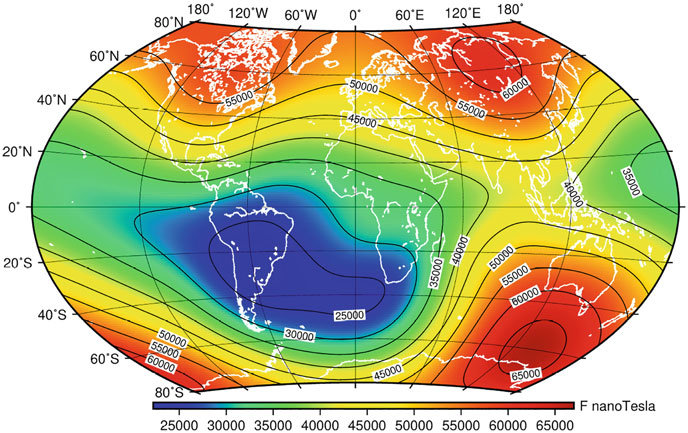
\includegraphics[width = 10cm]{Figures/IGRF-13th.png}
	\caption{The magnitude of geomagnetic field according to the 13th generation of the IGRF model~\cite{koskinen2022radiation}.}
	\label{fig:IGRF13th}
\end{figure*}

\section{Sensor models}
The positioning of the sensors on the satellite is necessary to meet mission requirements. The exact position of the sensors also impact the modelling of the anomalies on the sensors. Therefore, each sensors position on the satellite is provided as well as the measured vector of each sensor. It is further assumed that each sensor has a zero-mean Guassian noise and consequently, the low frequency noise such as drift is negligible. The sensor measurement in the SBC frame, $\mathbf{v}_{\mathcal{B}}$,  can be calculated as
\begin{equation}
\mathbf{v}_{\mathcal{B}} = \boldsymbol{A}^{\mathcal{B}}_{\mathcal{O}} \mathbf{v}_\mathcal{O} + \mathbf{m}_v,
\end{equation}
where $\mathbf{m}_v$ is the measurement noise of the current sensor and $\mathbf{v}_{\mathcal{I}}$ is the reference ORC vector. The measured unit vectors of the sun as an example of the sensor measurements is shown in Figure~\ref{fig:SunSensorPlot} where the grey background sections of the graphs are the eclipse periods, while the sections with the white background is the sunlit phase of the orbit.

\begin{figure}[!htb]
	\centering
	\def\pgfwidth{7cm}
	\import{Figures/TexFigures/Predictor-None/Isolator-None/Recovery-None/EARTH_SUN-ORC-General CubeSat Model/None/}{Sun.pgf}
	
	\caption{Sun vector in SBC}
	\label{fig:SunSensorPlot}
\end{figure}

%\begin{figure}[!htb]
%	\centering
%	\def\pgfwidth{7cm}
%	\import{Figures/TexFigures/Predictor-None/Isolator-None/Recovery-None/EARTH_SUN-ORC-General CubeSat Model/None/}{Earth_large.pgf}
%	
%	\caption{Earth vector in SBC}
%	\label{fig:EarthSensorPlot}
%\end{figure}
%
%\begin{figure}[!htb]
%	\centering
%	\def\pgfwidth{7cm}
%	\import{Figures/TexFigures/Predictor-None/Isolator-None/Recovery-None/EARTH_SUN-ORC-General CubeSat Model/None/}{Magnetometer_large.pgf}
%	
%	\caption{Magnetometer in SBC}
%	\label{fig:MagnetometerPlot}
%\end{figure}

\section{Disturbance models}
\label{section: disturbance models}
During orbit a satellite is exposed to various disturbance torques. It is these torques that cause the modelled attitude to differ from the actual attitude. Therefore, these torques are modelled and are assumed to influence the attitude of the satellite continuously. Other disturbances that occur only with anomalies are discussed in Chapter~\ref{chap:Anomalies}. Some disturbances are excluded from the simulation environment and only the major sources of disturbance torques are modelled and discussed.

The first disturbance torque is that of the gyroscopic coupling which can be calculated with
\begin{equation}
\mathbf{N}_{gyro} = \boldsymbol{\dot{\omega}}_\mathcal{B}^\mathcal{I} \times (\mathbf{I}\boldsymbol{\dot{\omega}}_\mathcal{B}^\mathcal{I} + \mathbf{h}_w),
\end{equation}
where $h_w$ is the angular momentum of the reaction wheels. The other disturbance torques are discussed in more detail below.

\subsection{Gravity Gradient}
The gravity gradient is caused by both the centrifugal force on the satellite due to the orbit around the Earth as well as the gravitational force. The part of the satellite nearest to the Earth will experience the largest gravitational force and the smallest centrifugal force of the satellite. While the part of the satellite furthest from the Earth will experience the smallest gravitational force and the largest centrifugal force. According to \cite{wertz2012spacecraft} the gravity gradient disturbance torque, $\mathbf{N}_{gg}$ can be calculated as 
\begin{equation}
\boldsymbol{N}_{gg} = 3 \, \omega_\mathcal{O}^2 (\mathbf{z}_{\mathcal{B}} \times \mathbf{Iz}_{\mathcal{B}}).
\end{equation}
The orbit nadir vector is calculated as,
\begin{equation}
\mathbf{z}_{\mathcal{B}} = \boldsymbol{A}^{\mathcal{B}}_{\mathcal{O}} \begin{bmatrix} 0 & 0 & 1 \end{bmatrix}^T.
\end{equation}
Due to the design of the satellite and the positions of the solar panels, the equation for $\mathbf{N}_{gg}$ can not be simplified. The gravity gradient torque is the only torque that can be accurately modelled on-board the satellite, and therefore is also included in the model update of the EKF. $\mathbf{N}_{gg}$ in SBC is shown in Figure~\ref{fig:GravityGradientTorques}.

\begin{figure}[!htb]
	\centering
	\def\pgfwidth{10cm}
	\import{Figures/TexFigures/Predictor-None/Isolator-None/Recovery-None/EARTH_SUN-ORC-General CubeSat Model/None/}{Gravity Gradient Torques.pgf}
	
	\caption{Gravity Gradient Torque in SBC}
	\label{fig:GravityGradientTorques}
\end{figure}

\subsection{Aerodynamic Disturbance}
The aerodynamic disturbance torques are cause by air density in the atmosphere creating a force on each individual segment of the satellite~\cite{Steyn2014}. This is significant due to the low Earth orbit (LEO) of the satellite, where the atmospheric density is higher. Therefore, the aerodynamic disturbance torque, $\mathbf{N}_{aero}$ is a summation of all the torques created by the air force on each segment area, $A_i$. $\mathbf{N}_{aero}$ can therefore be calculated as

\begin{equation}
\begin{aligned}
\mathbf{N}_{aero} = \sum_{i=1}^{n}\Big(& \rho \norm{\mathbf{v}_{\mathcal{B}}}^2 A_i H \{\text{cos}(\alpha_i)\} \, \text{cos}(\alpha_i) \big(\sigma_t (\mathbf{r}_{pi} \times \mathbf{\bar{v}}_{\mathcal{B}}) \\
					 & + \big[ \sigma_nS + (2 - \sigma_n - \sigma_t) \text{cos}(\alpha_i)\big] (\mathbf{r}_pi \times \mathbf{\bar{n}}_i) \big) \vphantom{\norm{\mathbf{v}_{\mathcal{B}}}^2}\Big),
\end{aligned}
\end{equation}
where $n$ is the number of segments of the satellite. The factors that influence the aerodynamic disturbance torque is the atmospheric velocity in SBC, $\mathbf{v}_{\mathcal{B}}$, the atmospheric density, $\rho$, each segment's surface area, $A_i$, and the offset vector between the segment's centre of mass (CoM) and the centre of pressure (CoP), $\mathbf{r}_p$. $H\{x\}$ is the Heaviside function which is equal to $0$ when $x$ is smaller than $0$ and otherwise equal to $1$. $\alpha_i$ is the incidence angle of $\mathbf{v}_{\mathcal{B}}$ on segment $i$, while $\sigma_t$ is the tangential accommodation coefficient and $\sigma_n$ is the normal accommodation coefficient. $S$ is the ratio of molecular exit velocity to $\mathbf{v}_{\mathcal{B}}$ and $\mathbf{\bar{n}}_i$ is the unit inward normal vector of segment $i$ \cite{JansevanVuuren2015}.

The atmospheric density is a function of the distance from the Earth surface. The density model provided by \cite{vallado2001fundamentals} is given as 
\begin{equation}
\rho = \rho_o e^{-\frac{h(t)-h_o}{H}},
\end{equation}
where $\rho_o$ is the reference density at the reference altitude, $h_o$, and $h(t)$ is the satellite's altitude as a function of time and $H$ is the scale height. According to \cite{steyn2011CubeSat} the atmospheric density is $\frac{1}{2}\rho$ during eclipse. Furthermore $\mathbf{v}_{\mathcal{B}}$ is calculated as
\begin{equation}
\begin{aligned}
\mathbf{v}_{\mathcal{B}} &= \boldsymbol{A}^{\mathcal{B}}_{\mathcal{O}} \boldsymbol{A}_{\mathcal{E}}^{\mathcal{O}} \mathbf{v}_{\mathcal{E}} \\
\text{where}  \qquad \mathbf{v}_{\mathcal{E}} &= \begin{bmatrix} 0 \\ 0 \\ \omega_E \end{bmatrix} \times \mathbf{r}_{sat} - \mathbf{v}_{sat}.
\end{aligned}
\end{equation}

$\sigma_n$ and $\sigma_t$ are both assumed to be equal to 0.8, while $S$ is $\num{0.8}$~\cite{steyn2011CubeSat}. From these equations the aerodynamic disturbance can be calculated and is shown in Figure~\ref{fig:AerodynamicTorques}.
\begin{figure}[!htb]
	\centering
	\def\pgfwidth{10cm}
	\import{Figures/TexFigures/Predictor-None/Isolator-None/Recovery-None/EARTH_SUN-ORC-General CubeSat Model/None/}{Aerodynamic Torques.pgf}
	
	\caption{Aerodynamic Torques in SBC}
	\label{fig:AerodynamicTorques}
\end{figure}

\subsection{Wheel Imbalance}
The reaction wheel imbalance is considered to be the most significant disturbance on the reaction wheel and consequently, only this disturbance torque is modelled for this simulation~\cite{bialke1998high}. Although reaction wheels are manufactured with low tolerances the reaction wheel will have a slight imbalance, since the mass of the reaction wheel will not be perfectly uniform and evenly displaced. 

The static imbalance of the reaction wheel is caused by the reaction wheel CoM offset from the rotational axis. Therefore, to model the static imbalance of the reaction wheels it is assumed that the unevenly distributed mass of the reaction wheel can be simplified to a point mass, $m$, a distance, $r$ from the rotational axis as shown in Figure~\ref{fig:StaticImbalance}. The static imbalance, $U_s$ is equal to $mr$ and this value is provided by the reaction wheel manufacturers.

\begin{figure}[!htb]
	\centering
	\def\svgwidth{10cm}
	\import{Figures/}{StaticImbalance.pdf_tex}
	\caption{Static Imbalance}
	\label{fig:StaticImbalance}
\end{figure}

To determine the resulting torque from the wheel imbalance the torque generated by each wheel is individually calculated. Consequently, for the reaction wheel in direction $\bar{x}_\mathcal{B}$, $RW_{\bar{x}_\mathcal{B}}$, the force, $F_{s\bar{x}_\mathcal{B}}$, generated by $U_s$ is dependent on the the angular rate, $\omega$, of the reaction wheel as well as the current position of $m$. Therefore, $F_{s\bar{x}_\mathcal{B}}$ can be expressed as

\begin{equation}
\mathbf{F}_{s\bar{x}_\mathcal{B}} = U_s\omega^2 \begin{bmatrix} 0 \\ \text{sin}(\omega t + \phi_s) \\ \text{cos}(\omega t + \phi_s)\end{bmatrix},
\end{equation}

where the current angle of $m$ is defined as $\omega t + \phi_s$, with $\phi_s$ as an arbitrary phase and for the sake of simplification is set to $0$. With $F_{s\bar{x}_\mathcal{B}}$ exerted on $RW_{\bar{x}_\mathcal{B}}$ known, the torque on the satellite can be calculated with the known position vector, $\mathbf{w}_{\bar{x}_\mathcal{B}}$, of $F_{s\bar{x}_\mathcal{B}}$ to the satellite CoM. Therefore, $N_{s\bar{x}_\mathcal{B}}$ can be calculated as

\begin{equation}
\mathbf{N}_{s\bar{x}_\mathcal{B}} = \mathbf{w}_{\bar{x}_\mathcal{B}} \times F_{s\bar{x}_\mathcal{B}}.
\end{equation}

This is calculated for each reaction wheel to determine the resulting static imbalance disturbance torque on the satellite. Another aspect of the reaction wheel imbalance is also modelled, namely the dynamic imbalance. The dynamic imbalance is caused by the principal inertia of the reaction wheel being misaligned with the rotational axis. This can be simplified to two equal point masses, $m$, with an axial displacement, $d$, and distance, $r$, from the rotational axis. These two masses are $\num{180}^o$ apart with respect to the rotational axis and consequently create two forces equal in magnitude and in opposite directions. The dynamic imbalance is graphically represented in Figure~\ref{fig:DynamicImbalance}.

\begin{figure}[!htb]
	\centering
	\def\svgwidth{10cm}
	\import{Figures/}{DynamicImbalance.pdf_tex}
	\caption{Dynamic Imbalance}
	\label{fig:DynamicImbalance}
\end{figure}

The dynamic wheel imbalance torque, $\mathbf{N}_{d\bar{x}_\mathcal{B}}$, for $RW_{\bar{x}_\mathcal{B}}$ can be calculated as 
\begin{equation}
\mathbf{N}_{d\bar{x}_\mathcal{B}} = U_d\omega^2 \begin{bmatrix} 0 \\ \text{sin}(\omega t + \phi_d) \\ \text{cos}(\omega t + \phi_d)\end{bmatrix}.
\end{equation}
where $U_d = mrd$ as the dynamic imbalance. Both $U_d$ and $U_s$ are provided by the manufacturer and based on the reaction wheel, RW-0.06 from Sinclair Interplanetary, $U_d = 2.08e^{-9}$ and $U_s = 2.08e^{-7}$. The net wheel imbalance torque from both the static and dynamic wheel imbalance is provided in Figure~\ref{fig:Wheel disturbance Torques}.

\begin{figure}[!htb]
	\centering
	\def\pgfwidth{10cm}
	\import{Figures/TexFigures/Predictor-None/Isolator-None/Recovery-None/EARTH_SUN-ORC-General CubeSat Model/None/}{Wheel disturbance Torques.pgf}
	
	\caption{Wheel disturbance torques in SBC}
	\label{fig:Wheel disturbance Torques}
\end{figure}

\section{Attitude Determination}
This section discusses the estimation algorithm for attitude determination of the satellite. This is done with the EKF, which utilizes the sensor measurements as well as modelled vectors according to physical models to estimate the current attitude. The EKF is highly sensitive to sensor anomalies and actuator failures and this section discusses the implementation of the EKF.

\subsection{Extended Kalman Filter}
The implementation of the EKF is for estimation of the current satellite attitude with sensor fusion of the magnetometer, star tracker, sun sensor and nadir sensor to accurately estimate the attitude and rotation rate of the satellite. The EKF will be used due to the non-linear nature of the system. The EKF consists of two fundamental parts, the model update and the measurement update. The estimated state vector, $\mathbf{x}$, will be denoted as $\hat{\mathbf{x}}$ and the estimated vector before and after the measurement update will be indicated with a superscript $'-'$ and $'+'$ respectively. The general form for a system model can be expressed as
\begin{equation}
	\mathbf{\dot{x}}_t} = \mathbf{f}(\mathbf{x}_t) + s_t,
\end{equation}
where $\mathbf{f}(\mathbf{x}_t)$ is a non-linear function of $\mathbf{x}_t$. To linearise $\mathbf{x}_t$ an approximation of $\mathbf{f}(\mathbf{x}_t)$ according to the Taylor series expansion is implemented.

\begin{equation}
\begin{aligned}
\mathbf{f}(x_t) &= \mathbf{f}(\hat{\mathbf{x}}_t) + \left[\frac{\partial \mathbf{f}}{\partial \hat{\mathbf{x}}_t} \right] \left(\mathbf{x}_t - \hat{\mathbf{x}}_t \right) + \frac{1}{2!} \left[\frac{\partial^2 \mathbf{f}}{\partial \hat{\mathbf{x}}_t^2} \right] \left(\mathbf{x}_t - \hat{\mathbf{x}}_t \right)^2 \\
				&\approx \mathbf{f} (\hat{\mathbf{x}}_t) + \mathbf{F} \Delta \mathbf{x}_t , \\
\text{where} \qquad \mathbf{F}_t &= \left[\frac{\partial \mathbf{f}}{\partial \hat{\mathbf{x}}_t} \right] \\
\text{and} \qquad \Delta \mathbf{x}_t &= \mathbf{x}_t - \hat{\mathbf{x}}_t. \\
\end{aligned}
\end{equation}


To linearise the state vector, $\mathbf{x}$, for the full 7-state EKF consists of the quaternion vector, $\mathbf{q}$ and the inertial-referenced angular velocity, $\boldsymbol{\omega}_{\mathcal{B}}^{\mathcal{I}}$ given as
\begin{equation}
	\mathbf{x} = [\mathbf{q}, \boldsymbol{\omega}_{\mathcal{B}}^{\mathcal{I}}]^T.
\end{equation}
To calculate the model update the dynamics and kinematics of the system model is used to calculate both $\boldsymbol{\omega}_{\mathcal{B}}^{\mathcal{I}}$ and $\mathbf{q}$. The integration method used in the simulation is the 4th order Runge-Kutta method to solve the differential equations. The integration method is shown in Algorithm~\ref{alg: Runge-Kutta} where $(\boldsymbol{\hat{\omega}}_{\mathcal{B}}^{\mathcal{I}})_k^-$ is calculated for the first step of the model update.

\begin{algorithm}[!htb]
	\caption[Runge-Kutta]{Runge-Kutta 4th order Algorithm at time $k$}
	\label{alg: Runge-Kutta}
	\begin{algorithmic}[1]
		\State Satellite Body Inertia $\mathbf{J} = \begin{bmatrix}
			0.4 & 0 & 0\\
			0 & 0.45 & 0 \\
			0 & 0 & 0.3
		\end{bmatrix}$
		\State Timestep ($T_s$) $= 1s$
		\State Number of iterations ($I$) $= 10$
		\State Step size $h = \frac{T_s}{I}$
		\State Disturbance torques $\mathbf{N}_d = N_{gg} - N_{gyro} $ % + N_{aero} + N_{rw}$
		\State Control torques $\mathbf{N}_c = N_m - N_w$
		\State $\mathbf{N} = \mathbf{N}_c + \mathbf{N}_d$
		\For{$n \coloneqq 1$ \textbf{to} $I$}
		\State \texttt{$k_1 = h(\mathbf{J^{-1}}\mathbf{N})$}
		\State \texttt{$k_2 = h(\mathbf{J^{-1}}\mathbf{N} + \frac{k1}{2})$}
		\State \texttt{$k_3 = h(\mathbf{J^{-1}}\mathbf{N} + \frac{k_2}{2})$}
		\State \texttt{$k_4 = h(\mathbf{J^{-1}}\mathbf{N} + k_3)$}
		\State \texttt{$\boldsymbol{\omega}_{n+1}=\boldsymbol{\omega}_n + \frac{k_1}{6} + \frac{k_2}{3} + \frac{k_3}{3} + \frac{k_4}{6}$}
		\EndFor
		\State $(\boldsymbol{\hat{\omega}}_{\mathcal{B}}^{\mathcal{I}})_k^- = \boldsymbol{\omega}_{n+1}$
		\State \textbf{return} $(\boldsymbol{\hat{\omega}}_{\mathcal{B}}^{\mathcal{I}})_k^-$
	\end{algorithmic}
\end{algorithm}
%\begin{equation}
%	f(x,y) = \mathbf{J^{-1}}\big((N_m)_{k-1} - (N_w)_{k-1} - (N_{gg})_{k-1} - (N_{gyro})_{k-1} \big)
%\end{equation}
With reference to \cite{JansevanVuuren2015}, $\hat{\mathbf{q}}_k^-$ can be calculated as

\begin{equation}
	\begin{aligned}
		\hat{\mathbf{q}}_k^- &= \left[\text{cos}(k_q)\mathbf{I}_{4 \times 4} + \frac{1}{\lVert (\boldsymbol{\hat{\omega}}_{\mathcal{B}}^{\mathcal{O}})_k^- \rVert} \text{sin}(k_q) \mathbf{\Omega}_k^- \right] \hat{\mathbf{q}}_{k-1}^+ \\ \\
		\text{where } k_q &= \frac{Ts}{2} \lVert (\boldsymbol{\hat{\omega}}_{\mathcal{B}}^{\mathcal{O}})_k^- \rVert \\ \\
		(\boldsymbol{\hat{\omega}}_{\mathcal{B}}^{\mathcal{O}})_k^- &= (\boldsymbol{\hat{\omega}}_{\mathcal{B}}^{\mathcal{I}})_k^- - \boldsymbol{\hat{A}}^{\mathcal{B}}_{\mathcal{O}_k} \begin{bmatrix} 0 & -(\omega_\mathcal{O})_k & 0\end{bmatrix}^T \\
		&= \begin{bmatrix} \boldsymbol{\hat{\omega}}_{\bar{x}_{\mathcal{O}}} & \boldsymbol{\hat{\omega}}_{\bar{y}_{\mathcal{O}}}  & \boldsymbol{\hat{\omega}}_{\bar{z}_{\mathcal{O}}} \end{bmatrix}^T \\ \\
		\lVert (\boldsymbol{\hat{\omega}}_{\mathcal{B}}^{\mathcal{O}})_k^- \rVert &= \sqrt{\boldsymbol{\hat{\omega}}_{\bar{x}_{\mathcal{O}}}^2 + \boldsymbol{\hat{\omega}}_{\bar{y}_{\mathcal{O}}}^2 + \boldsymbol{\hat{\omega}}_{\bar{z}_{\mathcal{O}}}^2} \\ \\
		\text{and } \mathbf{\Omega}_k^- &= \begin{bmatrix} 
			0 & \boldsymbol{\hat{\omega}}_{\bar{z}_{\mathcal{O}}} & -\boldsymbol{\hat{\omega}}_{\bar{y}_{\mathcal{O}}} & \boldsymbol{\hat{\omega}}_{\bar{x}_{\mathcal{O}}} \\
			-\boldsymbol{\hat{\omega}}_{\bar{z}_{\mathcal{O}}} & 0 & \boldsymbol{\hat{\omega}}_{\bar{x}_{\mathcal{O}}} & \boldsymbol{\hat{\omega}}_{\bar{y}_{\mathcal{O}}}			\\
			\boldsymbol{\hat{\omega}}_{\bar{y}_{\mathcal{O}}} & -\boldsymbol{\hat{\omega}}_{\bar{x}_{\mathcal{O}}} & 0 & \boldsymbol{\hat{\omega}}_{\bar{z}_{\mathcal{O}}}			\\
			-\boldsymbol{\hat{\omega}}_{\bar{x}_{\mathcal{O}}} & -\boldsymbol{\hat{\omega}}_{\bar{y}_{\mathcal{O}}} & -\boldsymbol{\hat{\omega}}_{\bar{z}_{\mathcal{O}}} & 0			\\
		\end{bmatrix}
	\end{aligned}
	\label{eq:q-propagation}
\end{equation}

The estimated state vector, $\hat{\mathbf{x}}_k^-$ can now be expressed as 

\begin{equation}
	\hat{\mathbf{x}}_k^- = \begin{bmatrix} (\boldsymbol{\hat{\omega}}_{\mathcal{B}}^{\mathcal{I}})_k^- & \hat{\mathbf{q}}_k^-\end{bmatrix}
\end{equation}
\textbf{TODO: $\mathbf{Q}_k$ is the covariance matrix representing the discrete system noise and is assumed to be zero-mean and Guassian. $\Phi_k$ is the discrete system perturbation model. $\mathbf{H}_k$ is the discrete measurement perturbation Jacobian Matrix. $\mathbf{R}_k$ is the measurement noise covariance matrix.}

The state covariance matrix $\mathbf{P}_k$ can be propagated as
\begin{equation}
	\mathbf{P}_k^- = \Phi_k \mathbf{P}_{k-1}^+ \Phi_k ^T.
	\label{eq:P_k}
\end{equation}
The error, $\mathbf{e}_k$, between the measured and modelled vector is calculated as
\begin{equation}
	\mathbf{e}_k = \mathbf{v}_\mathcal{B} - \boldsymbol{\hat{A}}^{\mathcal{B}}_{\mathcal{O}_k} \mathbf{v}_\mathcal{O}.
	\label{eq:errorVector}
\end{equation}
where $\mathbf{v}_\mathcal{B}$ is the measured vector in SBC and $\mathbf{v}_\mathcal{O}$ is the modelled ORC vector. The gain matrix $\mathbf{K}_k$ is used to determine the influence of $\mathbf{e}_k$ on the updated state vector, $\hat{\mathbf{x}}_k^+$. $\mathbf{K}_k$ can be calculated as 
\begin{equation}
	\mathbf{K}_k = \mathbf{P}_k^- (\mathbf{H}_k^-)^T \left[\mathbf{H}_k^- \mathbf{P}_k^- (\mathbf{H}_k^-)^T + \mathbf{R}_k \right]^{-1}.
\end{equation}
after which the updated state vector can be calculated as
\begin{equation}
	\hat{\mathbf{x}}_k^+ = \hat{\mathbf{x}}_k^- + \mathbf{K}_k \mathbf{e}_k.
	\label{eq:UpdatedStateVector}
\end{equation}
The state covariance matrix can then be updated as
\begin{equation}
	\mathbf{P}_k^+ = \left[\mathbf{I}_{7 \times 7} - \mathbf{K}_k \mathbf{H}_k^+ \right]\mathbf{P}_k \left[\mathbf{I}_{7 \times 7} - \mathbf{K}_k \mathbf{H}_k^+ \right] + \mathbf{K}_k \mathbf{R}_k \mathbf{K}_k^T.
	\label{eq:Updated_P_k}
\end{equation}
Where $\Phi_k$ is the discrete system perturbation model is calculated as
\begin{equation}
\begin{aligned}
\Phi_k &= \left[e^{T_s\mathbf{F}_t}\right]_{\mathbf{x}=\mathbf{\hat{x}},\quad t = kT_s} \\
\text{and simplified as} \qquad \Phi_k &\approx \left[\mathbf{I} + T_s\mathbf{F}_t + \frac{1}{2!}T_s^2\mathbf{F}_t^2\right]_{\mathbf{x}=\mathbf{\hat{x}},\quad t = kT_s}, \\
\end{aligned}
\end{equation}
according to \cite{Steyn2004Notes}. To validate the results of the EKF, the estimation error is given in Figure~\ref{fig:Estimation Metric}. Where the estimation error is the difference between the current $\mathbf{q}$ and $\mathbf{\hat{q}}$ in degrees.

\begin{figure}[!htb]
	\centering
	\def\pgfwidth{10cm}
	\import{Figures/TexFigures/Predictor-None/Isolator-None/Recovery-None/EARTH_SUN-ORC-General CubeSat Model/None/}{Estimation Metric.pgf}
	
	\caption{Estimation Metric}
	\label{fig:Estimation Metric}
\end{figure}

During the measurement update $\mathbf{e}_k$ is largely affected by anomalous behaviour in the sensor measurements. The sensitivity of the Kalman filter to the various anomalies is discussed in Chapter~\ref{chap:Anomalies}.

\section{Attitude Control}
To ensure that the satellite is able to satisfy the mission requirements, control of the satellite attitude is required. Therefore, the satellite's payload must be in the direction of the Earth during eclipse and the solar panels should be pointing in the direction of the sun during the sunlit phase. For this a quaternion feedback controller of the reaction wheels is implemented and a momentum dumping with the magnetorquers is implemented to ensure that the wheel disturbance remains within reasonable boundaries.

\subsection{Quaternion Feedback Controller}
\label{section: Quaternion Feedback Controller}
To ensure that the satellite is in the desired orientation with stable control in all three axes the quaternion feedback reaction wheel controller is implemented~\cite{wie1989quarternion}. The controller is provided with $\mathbf{\hat{x}}$ as input and outputs $\mathbf{N}_w$. To calculate the required torque, $\mathbf{N}_{w}$, the definition according to \cite{steyn2008attitude} for all cases at time step, $k$, is given as
\begin{equation}
	\mathbf{N}_{w} = K_{PI}\mathbf{Jq}_{err} + K_{DI}\mathbf{I}\hat{\boldsymbol{\omega}}_{\mathcal{B}}^{\mathcal{O}} - \hat{\boldsymbol{\omega}}_{\mathcal{B}}^{\mathcal{I}} \times \left[\mathbf{J}\hat{\boldsymbol{\omega}}_{\mathcal{B}}^{\mathcal{I}} + \mathbf{h}_{w}\right],
\end{equation}
where $\mathbf{h}_{w}$ is the measured angular momentum of the wheels and the control gains are defined as
\begin{equation}
	\begin{aligned}
		K_{PI} &= 2 \omega_n^2\\
		K_{DI} &= 2 \zeta \omega_n. \\
	\end{aligned}
	\label{eq:controlGain}
\end{equation}
The quaternion error, $\mathbf{q}_{err}$, is calculated with the quaternion difference operator, $\Theta$, as
\begin{equation}
	\begin{aligned}
		\mathbf{q}_{err} &= \mathbf{q_c} \Theta \hat{\mathbf{q}} \\
		\begin{bmatrix} 
			q_{1e} \\
			q_{2e} \\
			q_{3e} \\
			q_{4e}
		\end{bmatrix} &= \begin{bmatrix} 
			q_{4c} & q_{3c} & -q_{4c} & -q_{4c} \\
			-q_{3c} & q_{4c} & q_{1c} & -q_{2c} \\
			q_{2c} & - q_{1c} & q_{4c} & -q_{3c} \\
			q_{1c} & q_{2c} & q_{3c} & q_{4c}
		\end{bmatrix}
		\begin{bmatrix} 
			\hat{q}_1 \\
			\hat{q}_2 \\
			\hat{q}_3 \\
			\hat{q}_4
		\end{bmatrix},
	\end{aligned}
	\label{eq:quaternionError}
\end{equation}
where $\hat{\mathbf{q}}$ is the current estimated quaternion and $\mathbf{q}_{c}$ is the command quaternion which is $\begin{Bmatrix}
	0 & 0 & 0& 1
\end{Bmatrix}^T$ during eclipse and during the sun following phase, the attitude command according to \cite{chen2000ground} can be calculated as 
\begin{equation}
	\mathbf{q}_c = \begin{bmatrix}
		\mathbf{u}_c \text{sin}(\frac{\delta}{2}) \\
		\text{cos}(\frac{\delta}{2})
	\end{bmatrix},
\end{equation}
where 
\begin{equation}
	\mathbf{u}_c = \frac{\mathbf{u}_{sp}^{\mathcal{B}} \times \mathbf{s}_o}{\norm{\mathbf{u}_{sp}^{\mathcal{B}} \times \mathbf{s}_o}}.
\end{equation}
$\mathbf{s}_o$ is the measured unit sun vector in ORC, and the main solar panel's position is denoted as a unit vector, $\mathbf{u}_{sp}^{\mathcal{B}}$. The angle between $\mathbf{u}_{sp}^{\mathcal{B}}$ and $\mathbf{s}_o$, $\delta$, can be calculated with the vector dot-product. This can then be used as the reference for the control. The reference $\boldsymbol{\omega}_{\mathcal{B}}^{\mathcal{I}}$ is always $[0, 0, 0]$. 

\begin{figure}[!htb]
	\centering
	\def\pgfwidth{10cm}
	\import{Figures/TexFigures/Predictor-None/Isolator-None/Recovery-None/EARTH_SUN-ORC-General CubeSat Model/None/}{Pointing Metric.pgf}
	
	\caption{Pointing Metric}
	\label{fig:Pointing Metric}
\end{figure}

\subsection{Momentum Dumping}
Momentum dumping is crucial to ensure that the wheel disturbance does not cause the system to become unstable. Momentum dumping is implemented during eclipse after the satellite is in a stable nadir-pointing attitude. The momentum dumping is implemented with magnetic torquers based on a Cross-Product controller. The magnetic dipole moment $\mathbf{M}$ is calculated as 
\begin{equation}
\mathbf{M} = \frac{\mathbf{e} \times \mathbf{B}}{\norm{\mathbf{B}_b}^2},
\end{equation}
where $\mathbf{B}_b$ is the geomagnetic field and the error vector, $\mathbf{e}$ can be calculated as
\begin{equation}
\mathbf{e} = -K_w(\mathbf{h_w} - \mathbf{h_{w,ref}})
\end{equation}
where $K_w$ is a positive gain. This momentum dumping is implemented $200s$ after sun-following phase is implemented, to ensure stable control and reduce the momentum in the reaction wheels. The magnetorquers torques are shown in Figure~\ref{fig:Magnetic Control Torques} and it is evident that when the satellite control changes from eclipse to sunlit and from sunlit to eclipse the magnetorquers compensate for the increase in reaction wheel torques and minimise the reaction wheel disturbance.

\begin{figure}[!htb]
	\centering
	\def\pgfwidth{10cm}
	\import{Figures/TexFigures/Predictor-None/Isolator-None/Recovery-None/EARTH_SUN-ORC-General CubeSat Model/None/}{Magnetic Control Torques.pgf}
	
	\caption{Magnetic Control Torques}
	\label{fig:Magnetic Control Torques}
\end{figure}


%\section{Constellations}
%Explain the design of the satellite constellations and the algorithms to run communicate between satellites.
%
%\begin{algorithm}
%	
%	\SetKwInOut{Input}{Input}
%	\SetKwInOut{Output}{Output}
%	
%	\SetKwData{Left}{left}
%	\SetKwData{This}{this}
%	\SetKwData{Up}{up}
%	\SetKwFunction{Union}{Union}
%	\SetKwFunction{FindCompress}{FindCompress}
%	
%	\Indm
%	\Input{Description of the input to the algorithm.}
%	\Output{Description of the output from the algorithm.}
%	\Indp
%	
%	\BlankLine
%	
%	\emph{Initialize hyperparameters}\;
%	Get initial data from satellite\\
%	Update positions of each satellite\\
%	\For{$i\leftarrow 1$ \KwTo $N$}{
%		Determine $k$-nearest satellites to $satellite_i$ from the positions\\
%		Select data from nearest satellites\\
%		Send nearest satellites predictions and data to $satellite_i$\\
%		Retrieve data from $satellite_i$ and fault predictions of $k$-nearest satellites\\
%	}
%	Update position of $satellite_i$\\
%	Update data of $satellite_i$
%	
%	\caption[Do not end short caption with full-stop]{Algorithm example}
%	\label{alg}
%	
%\end{algorithm}


%\section{Typical Faults}
%For the simulation of the satellite and the induced faults to train and test various anomaly detection methodologies a database of typical faults is required. \cite{tafazoli2009study} made a study of the percentage of failure per subsystem. 
%
%\subsection{Probability of Fault Occurence}
%The occurrence of a fault depends on the reliability of that equipment. \cite{Guo2014} studied the reliability of small satellites and calculated the parameters for the Weibull distribution based on real data. To model the probability of a fault to occur the probability density function is used \cite{Jones2017}.
%
%This probability however is small and for the training of the system the data is too sparse for the computational abilities of any regular PC. Thus the probability of a failure during training is fixed to $1/1000000$ to produce the data required for the anomaly detection with a million test samples.
%
%\subsection{Set of faults}
%A set of typical faults for the ADCS is shown in Table~\ref{ADCS fault table}. 
%
%\newpage
%\begin{sidewaystable}[]
%	\label{ADCS fault table}
%	\begin{tabular}{|l|c|l|l|l|l|}
%		\hline
%		\multicolumn{6}{|c|}{\textbf{Internal Faults}} \\ \hline
%		\textbf{Fault classes} &
%		\multicolumn{1}{l|}{\textbf{\begin{tabular}[c]{@{}l@{}}Failure rate \\ per hour\end{tabular}}} &
%		\textbf{Fault causes} &
%		\textbf{References} &
%		\textbf{Possible effect} &
%		\textbf{Possible permutations} \\ \hline
%		\multirow{4}{*}{Reaction wheels} &
%		\multicolumn{1}{l|}{\multirow{4}{*}{2.5E-7 \cite{Spilhaus1987}}} &
%		\begin{tabular}[c]{@{}l@{}}Reaction wheel electronics \\ fail\end{tabular} &
%		\cite{allen2012satellite} \cite{Jacklin2019} &
%		\begin{tabular}[c]{@{}l@{}}Does not respond \\ to control inputs\end{tabular} &
%		\begin{tabular}[c]{@{}l@{}}Momentum remains the same \\ or decreases slightly due to \\ friction\end{tabular} \\ \cline{3-6} 
%		&
%		\multicolumn{1}{l|}{} &
%		Overheated reaction wheel &
%		\cite{Wintoft} &
%		Decrease in speed &
%		1\% of initial speed per second \\ \cline{3-6} 
%		&
%		\multicolumn{1}{l|}{} &
%		\begin{tabular}[c]{@{}l@{}}Catastrophic failure (cause \\ unknown)\end{tabular} &
%		\cite{Choi2011} &
%		Stops rotating &
%		0 \\ \cline{3-6} 
%		&
%		\multicolumn{1}{l|}{} &
%		\begin{tabular}[c]{@{}l@{}}Increase in rotation speed \\ (Unknown cause)\end{tabular} &
%		\begin{tabular}[c]{@{}l@{}}Gerhard Janse \\ van Vuuren\end{tabular} &
%		\begin{tabular}[c]{@{}l@{}}Wheel speed \\ increases\end{tabular} &
%		\begin{tabular}[c]{@{}l@{}}Between 90-100\% of maximum \\ wheel speed\end{tabular} \\ \hline
%		Magnetorquers &
%		\multicolumn{1}{l|}{ADCS fault table8.15E-9 \cite{Spilhaus1987}} &
%		Polarities are inverted &
%		\cite{Crowell2011} &
%		Incorrect rotation &
%		\\ \hline
%		\multirow{2}{*}{Magnetometers} &
%		\multicolumn{1}{l|}{\multirow{2}{*}{8.15E-9 \cite{Spilhaus1987}}} &
%		Unknown &
%		\begin{tabular}[c]{@{}l@{}}Gerhard Janse \\ van Vuuren\end{tabular} &
%		Stops reacting &
%		\begin{tabular}[c]{@{}l@{}}Provides no feedback or the \\ output remains constant\end{tabular} \\ \cline{3-6} 
%		&
%		\multicolumn{1}{l|}{} &
%		\begin{tabular}[c]{@{}l@{}}Magnetometers and magne-\\ torquers interfered with \\ each other\end{tabular} &
%		\cite{Jacklin2019} &
%		\begin{tabular}[c]{@{}l@{}}Noise on magneto-\\ meters and noise \\ on control of mag-\\ netorquers\end{tabular} &
%		\begin{tabular}[c]{@{}l@{}}Between x3 and x5 times the \\ normal noise magnitude \\ Guassian distribution\end{tabular} \\ \hline
%		Earth Sensor &
%		- &
%		Unknown &
%		\cite{Robertson2019} &
%		\begin{tabular}[c]{@{}l@{}}Noisy Earth Sensor \\ effected pointing \\ accuracy\end{tabular} &
%		\begin{tabular}[c]{@{}l@{}}Between x5 and x10 times the \\ normal sensor noise based on \\ Guassian distribution\end{tabular} \\ \hline
%		\multirow{2}{*}{Sun sensor} &
%		\multirow{2}{*}{-} &
%		\begin{tabular}[c]{@{}l@{}}Cross-wired during instal-\\ lation\end{tabular} &
%		\cite{Crowell2011} &
%		\begin{tabular}[c]{@{}l@{}}Erroneous \\ measurements\end{tabular} &
%		Uniform random values \\ \cline{3-6} 
%		&
%		&
%		Unknown &
%		\cite{Jacklin2019} &
%		Sun sensor fails &
%		output is 0 \\ \hline
%		Star tracker &
%		- &
%		\begin{tabular}[c]{@{}l@{}}Shutter on star tracker is \\ closed\end{tabular} &
%		\cite{Crowell2011} &
%		Star tracker fails &
%		output is 0 \\ \hline
%		Overall control &
%		- &
%		\begin{tabular}[c]{@{}l@{}}Incorrect control law or \\ variation \\ thereof\end{tabular} &
%		\begin{tabular}[c]{@{}l@{}}Gerhard Janse \\ van Vuuren\end{tabular} &
%		\begin{tabular}[c]{@{}l@{}}Angular velocity \\ suddenly increases \\ or decreases or \\ oscillation results\end{tabular} &
%		\begin{tabular}[c]{@{}l@{}}Increase to 75 - 100\% \\ Decrease to 0 - 25\%\\ Oscillates\end{tabular} \\ \hline
%		\multirow{3}{*}{\begin{tabular}[c]{@{}l@{}}Common data \\ transmission errors\end{tabular}} &
%		\multirow{3}{*}{-} &
%		Sign flip &
%		\cite{Crowell2011} &
%		Processor-based &
%		\begin{tabular}[c]{@{}l@{}}Processor outputs and/or \\ inputs experience a sign flip\end{tabular} \\ \cline{3-6} 
%		&
%		&
%		Bit flip &
%		N/A &
%		&
%		\begin{tabular}[c]{@{}l@{}}Processor outputs and/or \\ inputs experience a bit flip flip\end{tabular} \\ \cline{3-6} 
%		&
%		&
%		Insertion of zeros &
%		\cite{Jacklin2019} &
%		&
%		\begin{tabular}[c]{@{}l@{}}Processor outputs and/or inputs \\ experience an insertion of a zero\end{tabular} \\ \hline
%		\begin{tabular}[c]{@{}l@{}}Possible sensors \\ errors\end{tabular} &
%		- &
%		Unknown &
%		N/A &
%		High sensor noise &
%		\begin{tabular}[c]{@{}l@{}}Between x5 and x10 times the \\ normal sensor noise based on \\ Guassian distribution\end{tabular} \\ \hline
%	\end{tabular}
%\end{sidewaystable}
%
%\newpage
\chapter{Implementation of Methods on Actual Satellite}
\label{chap:Implementation of Methods on Actual Satellite}

\section{Fault Detection, Isolation and Recovery}

\section{Feature Extraction}

\section{Detection}

\section{Isolation}

\section{Recovery}

\section{Summary}
\chapter{Anomalies}
\label{chap:Anomalies}
To ensure that the prediction and classification of anomalies are not based on generalised sensor failures a few anomalies are simulated. These anomalies are either chosen to show the significant effect of these anomalies on the ADCS or are modelled based on research that label the anomaly as a possible influence on the ADCS. There is a anomaly for each sensor, that will create inaccuracies for that specific sensor measurement. An anomaly for the reaction wheels is also implemented to show the resulting estimation failure based on a inaccurate model update, since the control torque, $\mathbf{N}_w$ and the torque implemented on the reaction wheel is not the same. All anomalies will also be predicted based on the sensor readings and outputs from feature extractions, since the effect will be evident on all the sensors.

\section{Reflection of Solar Panels on Sun Sensor}
\label{section:Reflection}
The reflection anomaly is modelled for the specific shape and design of the satellite as shown in Figure~\ref{fig:CubeSatDesign}.  The modelling takes place within the satellite body coordinate (SBC) frame, $\mathcal{B}\{\bar{\mathbf{x}}_{\mathcal{B}},~\bar{\mathbf{y}}_{\mathcal{B}},~\bar{\mathbf{z}}_{\mathcal{B}}\}$.

%\begin{figure}[h!t!b]
%	\centering
%	\def\svgwidth{12cm}
%	\import{Figures/}{ReflectionModel.pdf_tex}
%	\caption{The modelled satellite, with solar panels and sun sensor within the SBC frame.}
%	\label{fig:CubeSat}
%\end{figure}

\begin{figure*}[h!t!b]
	\centering
	\def\svgwidth{7cm}
	\import{Figures/}{ReflectionModelPoint.pdf_tex}
	\centering
	\def\svgwidth{7cm}
	\import{Figures/}{LineIntersection.pdf_tex}
	\caption{Definition of solar reflection point from $ABCD$-plane.}
	\label{fig:LineIntersection}
\end{figure*}

The assumption is that the solar panel can be modeled as a geometric plane. Therefore, light from the solar panel will reflect similarly to a perfectly smooth mirror. This model also assumes, that if the sun sensor detects any reflection from the solar panel, the measured sun vector will default to the reflection ray instead of the direct sun vector. In practice, this is a function of the exact detection algorithm within the sensor, and some reflections might be ignored.  This assumption will produce the worst-case behaviour.  The intensity of the light vector is also disregarded.

The solar panel $ABCD$-plane can be represented in the SBC by a point and normal vector defined as
\begin{equation}
\begin{split}
\mathbf{p}_{ABCD} &= [p_x,~p_y,~p_z]^\top, \text{and}\\
\bar{\mathbf{n}}_{ABCD} &= [n_px,~n_py,~np_z]^\top,
\end{split}
\end{equation}
respectively.  Similarly, the sun sensor $WXYZ$-plane is represented by the point, $\mathbf{p}_{WXYZ}$, and normal vector, $\bar{\mathbf{n}}_{WXYZ}$.

The reflected sun vector, $\mathbf{r}_{\text{ref}}$, can be calculated by
\begin{equation}
\mathbf{r}_{\text{ref}} = \mathbf{r}_{\text{sun}} - 2\bar{\mathbf{n}}_{ABCD}^\top(\mathbf{r}_{\text{sun}} \cdot \bar{\mathbf{n}}_{ABCD}),
\end{equation}
where $\mathbf{r}_{\text{sun}}$ is the incoming sun vector.  To calculate the intersection of the reflected vector with the $WXYZ$-plane of the sun sensor, the equation of the $WXYZ$-plane, the reflected vector, and the point of origin is required. The reflection of the sun vector is illustrated in Figure~\ref{fig:LineIntersection}. The reflection from $Q$ to $Q'$ can thus be calculated as a projection of $\mathbf{r}_{\text{ref}}$ unto the $WXYZ$-plane.

To model reflection from the solar panels to the sun sensor, only two corners of the solar panel and two corners of the sun sensor are to be considered. From Figure~\ref{fig:LineIntersection} it is evident that if the solar panel reflects on $Y$ that the reflection will also cover $X$. The same is true for corner $Z$ and $W$. Since $C'$ will be at the same position as $C$, which is valid for $D'$ and $D$, the calculation can be omitted. Therefore it is only necessary to calculate the reflected positions $A'$ and $B'$. This simplifies the reflection model significantly.

The reflected position $A'$ can be calculated as the intersection of the reflected vector $R$ with plane $WXYZ$. We also know the position of $A$, based on the satellite design, and can therefore calculate $A'$. The same applies to $B$ and $B'$. To determine whether $Y$ or $X$ is within the reflection region, we assume that the plane $WXYZ$ is a 2D plane, and we omit the third dimension. Therefore, the axis changes from $x, y, z$ to only $x, y$. We calculate whether $x$ is between the lines of $A'D$ and $B'C$ and between the lines $CD$ and $A'B'$. By determining the line equation between reflected points in the form 
\begin{equation}
y_{A'B'} = mx_{A'B'} + c,
\label{eq:line equation}
\end{equation}
from the coordinates of $A'$ and $B'$, the corresponding $X_{A'B',y}$ can be calculated by substituting $X_x$ into Eq~\ref{eq:line equation}. With the same method the coordinates of $X_{B'C}$, $X_{A'D}$, $X_{A'B'}$ and $X_{CD}$ can be determined. After that, with logical if statements, it can be determined whether $X$ is in the reflection zone. If $X_x$ is to the right of $X_{B'C,x}$ and to the left of $X_{A'D,x}$, as well as $X_y$ is above $X_{A'B',y}$ and below $X_{CD,y}$ then $X$ is within the reflection zone. 

The results for the sun vector with and without reflection are shown in Figure~\ref{fig:Sun Vector comparison}. There is a clear difference between the true sun vector and the possible measurement influenced by the reflection.  This false reflection vector may affect the estimation and, thus also the attitude control of the satellite.

\begin{figure*}[!htb]
	\begin{subfigure}{.5\textwidth}
		\centering
%		 include first image
		\import{Figures/TexFigures/Predictor-None/Isolator-None/Recovery-None/EARTH_SUN-ORC-General CubeSat Model/Reflection/}{Sun.pgf}
%		\caption[Sun vector with reflection]{Sun vector with reflection.}
		\label{fig:Sun Vector comparison with reflection}
	\end{subfigure}
	\begin{subfigure}{.5\textwidth}
		\centering
		% include second image
		\import{Figures/TexFigures/Predictor-None/Isolator-None/Recovery-None/EARTH_SUN-ORC-General CubeSat Model/None/}{Sun.pgf} 
%		\caption[Sun vector without reflection]{Sun vector without reflection.}
		\label{fig:Sun Vector comparison without reflection}
	\end{subfigure}
	\caption{Comparison of measured sun vector with and without reflections (gray areas indicate the eclipse period of the orbit)}
	\label{fig:Sun Vector comparison}
	
\end{figure*}

%\begin{figure*}[!htb]
%	\begin{subfigure}{.5\textwidth}
%		\centering
%		% include first image
%		\import{Figures/TexFigures/}{Reflection-Sun.pgf}
%		\caption[Sun vector with reflection]{Sun vector with reflection.}
%		\label{fig:Sun Vector comparison with reflection}
%	\end{subfigure}
%	\begin{subfigure}{.5\textwidth}
%		\centering
%		% include second image
%		\import{Figures/TexFigures/}{None-Sun.pgf} 
%		\caption[Sun vector without reflection]{Sun vector without reflection.}
%		\label{fig:Sun Vector comparison without reflection}
%	\end{subfigure}
%	
%	\caption{Comparison of measured sun vector with and without reflections (gray areas indicate the eclipse period of the orbit)}
%	\label{fig:Sun Vector comparison}
%	
%\end{figure*}

%\begin{figure}[!htb]
%	\centering
%	\def\svgwidth{14cm}
%	\import{Figures/}{ReflectionModel.pdf_tex}
%	\caption{Cube Sat}
%	\label{fig:CubeSat}
%\end{figure}
%
%\begin{figure*}[!hbt]
%	\centering
%	\def\svgwidth{7cm}
%	\import{Figures/}{ReflectionModelPoint.pdf_tex}
%	\centering
%	\def\svgwidth{7cm}
%	\import{Figures/}{LineIntersection.pdf_tex}
%	\caption{Reflection}
%	\label{fig:LineIntersection}
%\end{figure*}
%
%The assumption is that the solar panel can be modelled as a geometric plane. Therefore, light from the solar panel will reflect as from a perfectly smooth mirror. It is further assumed that if the sun sensor detects any reflection from the solar panel, the measured sun vector will default to the reflection ray instead of the direct sun vector. Therefore the intensity of the light vector is disregarded. The reflected sun vector, $r$, can be calculated as
%\begin{equation}
%	\mathbf{r} = \mathbf{v} - 2\mathbf{n}^T(\mathbf{v} \cdot \mathbf{n}).
%\end{equation}
%Where $\mathbf{v}$ is the incoming sun vector and $\mathbf{n}$ is the average vector to the plane $ABCD$ of the solar panel, as seen in Figure~\ref{fig:CubeSat}. To calculate the intersection of the reflected vector with the plane $XWYZ$ of the sun sensor, the equation of the plane, $XWYZ$, the reflected vector, $r$, and the point of origin is required. The reflection of the sun vector, $\mathbf{v}$ is illustrated in Figure~\ref{fig:LineIntersection} The equation for a plane can be denoted as
%
%\begin{equation}
%	\mathbf{p} = ax + by + cz + d.
%	\label{eq:Plane}
%\end{equation}
%Where $x$, $y$ and $z$ are the dimensions in the SBC frame. The reflected unit vector can also be translated to 
%\begin{equation}
%	\begin{aligned}
%		&	x = \alpha t \\
%		&	y = \beta t \\
%		&	z = \zeta t \\
%	\end{aligned}
%	\label{eq:LineOfVector}
%\end{equation}
%Where the coefficients, $\alpha$, $\beta$ and $\zeta$ are the values of the reflected unit vector in each respective dimension. Since we can calculate the coefficients for Eq~\ref{eq:LineOfVector} from the reflected vector, we can calculate $t$, by substituting $x$, $y$ and $z$ into Eq~\ref{eq:Plane}. This is possible, because we determine the equation of the plane for the surface $XYZW$ based on our design. 
%
%After that, the intersecting point with the plane $XYZW$ can be calculated as
%\begin{equation}
%	P(x, y, z) = (o_1 + \alpha t, o_2 + \beta t, o_3 + \zeta t)
%	\label{eq:Intersection}
%\end{equation}
%where $o_1, o_2, o_3$ is the point of origin. Which in this case is the position of reflection from the solar panel. Therefore, if the sun vector $\mathbf{v}$ reflected from the solar panel as $\mathbf{r}$, the point of intersection $Q'$ on Figure~\ref{fig:LineIntersection} can be calculated as
%\begin{equation}
%	Q'(x, y, z) = (Q_x + \alpha t, Q_y + \beta t, Q_z + \zeta t)
%	\label{eq:SpecificIntersection}
%\end{equation}
%
%To model reflection from the solar panels to the sun sensor, only two corners of the solar panel and two corners of the sun sensor are to be considered. From Figure~\ref{fig:LineIntersection} it is evident that if the solar panel reflects on $Y$ that the reflection will also cover $X$. The same is true for corner $Z$ and $W$. Since $C'$ will be at the same position as $C$, which is valid for $D'$ and $D$, the calculation can be omitted. Therefore it is only necessary to calculate the reflected positions $A'$ and $B'$. This simplifies the reflection model significantly.
%
%The reflected position $A'$ can be calculated as the intersection of the reflected vector $R$ with plane $XYZW$ using Eq~\ref{eq:Intersection}. We also know the position of $A$, based on the satellite design and can therefore calculate $A'$. The same applies to $B$ and $B'$. To determine whether $Y$ or $X$ is within the reflection region, we assume that the plane $XYWZ$ is a 2D plane, and we omit the third dimension. Therefore, the axis changes from $x, y, z$ to only $x, y$. We calculate whether $x$ is between the lines of $A'D$ and $B'C$ and between the lines $CD$ and $A'B'$. By determining the line equation between reflected points in the form 
%\begin{equation}
%	y_{A'B'} = mx_{A'B'} + c
%	\label{eq:line equation}
%\end{equation}
%from the coordinates of $A'$ and $B'$, the corresponding $X_{A'B',y}$ can be calculated by substituting $X_x$ into Eq~\ref{eq:line equation}. With the same method the coordinates of $X_{B'C}$, $X_{A'D}$, $X_{A'B'}$ and $X_{CD}$ can be determined. After that, with logical if statements, it can be determined whether $X$ is in the reflection zone. If $X_x$ is to the right of $X_{B'C,x}$ and to the left of $X_{A'D,x}$, as well as $X_y$ is above $X_{A'B',y}$ and below $X_{CD,y}$ then $X$ is within the reflection zone. 
%
%The results for the sun vector with and without reflection is shown in Figure~\ref{fig:Sun Vector comparison}. During the modelling of the reflection, the reflection also affects the estimation and, therefore, the attitude control of the satellite. In the figures of this article, the grey zones indicate the eclipse period, as seen in Figure~\ref{fig:Sun Vector comparison}.
%
%\begin{figure*}[!htb]
%	\begin{tabular}{@{}c@{}}
%		\centering
%%		 include first image
%		\import{Figures/TexFigures/Predictor-None/Isolator-None/Recovery-None/EARTH_SUN-ORC-General CubeSat Model/Reflection/}{Sun.pgf}
%%		\caption[Sun vector with reflection]{Sun vector with reflection.}
%		\label{fig:Sun Vector comparison with reflection}
%	\end{tabular}
%	\begin{tabular}{@{}c@{}}
%		\centering
%		% include second image
%		\import{Figures/TexFigures/Predictor-None/Isolator-None/Recovery-None/EARTH_SUN-ORC-General CubeSat Model/None/}{Sun.pgf} 
%%		\caption[Sun vector without reflection]{Sun vector without reflection.}
%		\label{fig:Sun Vector comparison without reflection}
%	\end{tabular}
%	
%	\caption{Comparison of Sun Vector with and without Reflection}
%	\label{fig:Sun Vector comparison}
%	
%\end{figure*}

\subsection{Influence of Anomaly on Estimation}
To determine whether the reflection on the sun sensor has a influence on the ADCS, the estimation metric is shown in Figure~\ref{fig:reflectionEstimation}. The estimation metric, is the angle difference between the actual attitude and the estimated attitude. It is evident that the reflection has a large influence on the estimation when Figure~\ref{fig:reflectionEstimation} is compared with Figure~\ref{fig:Estimation Metric}. The maximum estimation error is $6^o$ for normal operation and it is evident in Figure~\ref{fig:reflectionEstimation} that the estimation error is sometimes even $150^o$. It is also clear that during the eclipse the estimation returns to a more accurate estimation. This is due to the fact that all sensors are ignored if the measured vector is $0$ and the sun vector is $0$ during eclipse.
\begin{figure}[!htb]
	\centering
	
	\import{Figures/TexFigures/Predictor-None/Isolator-None/Recovery-None/EARTH_SUN-ORC-General CubeSat Model/Reflection/}{Estimation Metric.pgf}
	
	\caption{Estimation Metric with reflection on sun sensor}
	\label{fig:reflectionEstimation}
\end{figure}

\section{Moon in Field of View of Nadir Sensor}
An anomaly that can be experienced by an infrared (IR) nadir sensor is the moon overlapping the horizon of the Earth in die nadir sensor's field of view (FoV). This is shown in Figure~\ref{fig:ProjectionOnPlane}. This influences the edge detection and circular fit algorithm \cite{wessels2018infrared, van2008infrared} and consequently the calculated centre of the Earth. Firstly, it is required to simulate the image seen by the nadir sensor, thereafter the algorithm for detecting the centre of the Earth can be implemented.

\subsection{Simulating Nadir Sensor Infra-red Image}
Firstly, the vectors of both the satellite to Earth, $\mathbf{R}_{SE}$ and the Earth to moon, $\mathbf{R}_EM$, is required. The moon position is determined with the Julian date, since the propagation of the moon position relative to the centre of the Earth has been calculated in advance. These vectors are shown in Figure~\ref{fig:EarthMoonSatPosition}. 

\begin{figure}[!htb]
	\centering
	\def\svgwidth{14cm}
	\import{Figures/}{EarthMoonSatPosition.pdf_tex}
	\caption{Earth to Moon and Earth to Satellite Vectors}
	\label{fig:EarthMoonSatPosition}
\end{figure}

From the vector, $\mathbf{R}_{SE}$, and the position of the centre of the Earth, $P_{Earth}$, a 3D plane normal to $\mathbf{R}_{SE}$ and at $P_{Earth}$ can be calculated. Where both $P_{Earth}$ and $\mathbf{R}_{SE}$ are defined as
\begin{equation}
	P_{Earth} = [\bar{\mathbf{x}}_{\mathcal{E}_0}, \bar{\mathbf{y}}_{\mathcal{E}_0}, \bar{\mathbf{z}}_{\mathcal{E}_0}],
\end{equation}
and  
\begin{equation}
	\mathbf{R}_{SE} = [\mathbf{n}_{\bar{\mathbf{x}}_{\mathcal{E}}}, \mathbf{n}_{\bar{\mathbf{y}}_{\mathcal{E}}}, \mathbf{n}_{\bar{\mathbf{z}}_{\mathcal{E}}}].
\end{equation}
Therefore with the equation for the 3D plane defined as 
\begin{equation}
A\bar{\mathbf{x}}_{\mathcal{E}} + B\bar{\mathbf{y}}_{\mathcal{E}} + C{\bar{\mathbf{x}}_{\mathcal{E}}} = Dm
\end{equation}
where the parameters $A, B, C, D$ can be calculated as
\begin{equation}
\begin{bmatrix}
	A\\
	B\\
	C\\
	D\\
\end{bmatrix} = \begin{bmatrix}
\mathbf{n}_{\bar{\mathbf{x}}_{\mathcal{E}}} \\ \mathbf{n}_{\bar{\mathbf{y}}_{\mathcal{E}}} \\ \mathbf{n}_{\bar{\mathbf{z}}_{\mathcal{E}}} \\
\mathbf{n}_{\bar{\mathbf{x}}_{\mathcal{E}}}\bar{\mathbf{x}}_{\mathcal{E}_0} + \mathbf{n}_{\bar{\mathbf{y}}_{\mathcal{E}}}\bar{\mathbf{y}}_{\mathcal{E}_0} + \mathbf{n}_{\bar{\mathbf{z}}_{\mathcal{E}}}\bar{\mathbf{z}}_{\mathcal{E}_0} \\
\end{bmatrix}
\end{equation}
This 3D plane slicing the Earth in half as seen from the satellite is shown in Figure~\ref{fig:PlaneThroughEarth}. The moon and Earth can both be projected unto the 3D plane to determine the image seen by the nadir sensor. Therefore the nadir vector must also be projected unto the 3D plane. A circle can be drawn for the Earth, moon and the nadir sensor's FoV. The radius, of the moon as projected on the 3D plane can be calculated as 

\begin{equation}
	R_{moon} = \norm{\mathbf{R}_{SE}} \frac{r_{moon}}{\norm{\mathbf{R}_{SM}}}
\end{equation}

the radius of the nadir sensor FoV, $R_{FoV}$ can calculated as 

\begin{equation}
	R_{FoV} = \norm{\mathbf{R}_{SE}} \tan\left(\theta \right)
\end{equation}

With these variables defined and calculated, the edges of the moon and Earth within the nadir FoV can be determined.

% Update the image that Rse should be the vector from the nadir sensor (SBC to ORC)
% because the vector is normal to the plane, the depth coordinate can be ignored

\begin{figure}[!hbt]
	\centering
	\def\svgwidth{14cm}
	\import{Figures/}{PlaneThroughEarth.pdf_tex}
	\caption{Plane perpendicular to $\mathbf{R}_{SE}$ and at center of Earth}
	\label{fig:PlaneThroughEarth}
\end{figure}

Firstly the edges of the moon and Earth are discretely determined due to the pixel width of the nadir sensor. The discrete points are therefore based on a fixed number of points for the Earth, $N$, and the number of discrete points on the moon is determined based on the ratio of $R_{moon}$ to $R_{Earth}$. The discrete points for the moon is therefore equal to $N \left(\frac{R_{moon}}{R_{Earth}} \right)$. The projected Earth and moon as discrete points unto the 3D plane is shown in Figure~\ref{fig:ProjectionOnPlane}. The discrete edges of the Earth and moon that is within the FoV will be used for the algorithm to calculate the centre of the earth as discussed in Section~\ref{section: Calculating the Centre of the Earth}. The discrete points from the earth used must satisfy the following conditions:
\begin{enumerate}
	\item Distance between point and centre of nadir Sensor FoV must be smaller than $R_{FoV}$.
	\item Distance between point and centre of moon must be larger than $R_{moon}$.
\end{enumerate}
The discrete edges of the moon used for the algorithm must satisfy the following conditions:
\begin{enumerate}
	\item Distance between any discrete point and centre of Earth must be smaller than $R_{Earth}$ for the moon to overlap the horizon.
	\item Distance between point and centre of nadir Sensor FoV must be smaller than $R_{FoV}$.
	\item Distance between point and centre of Earth must be larger than $R_{Earth}$.
\end{enumerate}
This the creates the array of points that will be used in the algorithm to calculate the centre of the Earth.

\begin{figure}[!hbt]
	\centering
	\def\svgwidth{14cm}
	\import{Figures/}{ProjectionOnPlane.pdf_tex}
	\caption{Projection of moon and Earth on plane}
	\label{fig:ProjectionOnPlane}
\end{figure}

\textbf{TODO: Fix green arrow and text of Rmoon on Figure}

\subsection{Calculating the Centre of the Earth}
\label{section: Calculating the Centre of the Earth}
The edges of the Earth are detected based on a gradient between the lowest temperature and the highest temperature within the IR nadir sensor's FoV. This will not be implemented in our case, since we can determine discrete points of both the Earth and the moon from the simulation environment. Furthermore the visible phases of the moon will not be accounted for. The reasoning for this is due to the coldest side of the moon being $140$K and the warmest part, $400$K. The temperature of space is $\num{2.7}$K and the coldest part on the Earth is $180$K. Consequently, the IR horizon sensor must be calibrated to always use the minimum value for edge detection as $180$K or it must use the smallest value in the image, which will most likely be $2.7$K. Therefore, it can be assumed that the moon will not have any detectable phases for the IR horizon sensor and it will always be seen as a full moon, due to it's lowest temperature being warmer than that of space. 

With this assumption the circular fit algorithm as shown in Figure~\ref{fig:CircularFit} can now be used to determine the centre of the Earth on the plane \cite{wessels2018infrared}. For this calculation the $3$D plane is transformed to a $2$D plane and all the coordinates is also transformed. The centre of the Earth on the 2D plane is therefore given as $\left(x_c, y_c\right)$. The goal of the algorithm is to calculate $\left(x_c, y_c\right)$ and use it to transform the point to the 3D plane and thereafter calculate the $\mathbf{R}_{SE}$.

\begin{figure}[!hbt]
	\centering
	\def\svgwidth{14cm}
	\import{Figures/}{CircularFit.pdf_tex}
	\caption{Circular Fit Algorithm}
	\label{fig:CircularFit}
\end{figure}

Firstly the curvature of a circle is described as 
\begin{equation}
	ax + by + c = x^2 + y^2,
\end{equation}
where 
\begin{equation}
	\begin{aligned}
		a &= 2x_c \\
		b &= 2y_c \\
		c &= r_c^2-\sqrt{x_c^2 + y_c^2}.
	\end{aligned}
\end{equation}
Therefore using all the coordinates of discrete edges, $(x_n, y_n)$, within the nadir sensor FoV, $a$, $b$ and $c$ can be calculated as
\begin{equation}
	\begin{bmatrix}
		x_0 & y_0 & 1\\
		x_1 & y_1 & 1\\
		\vdots & \vdots & \vdots\\
		x_n & y_n & 1\\
	\end{bmatrix}	\begin{bmatrix}
	a\\
	b\\
	c
\end{bmatrix} = \begin{bmatrix}
		x_0^2 + y_0^2\\
		x_1^2 + y_1^2\\
		\vdots \\
		x_n^2 + y_n^2\\
	\end{bmatrix}.
\end{equation}
It is thus evident that when the moon overlaps the horizon of the Earth from the nadir sensor's perspective the centre of the Earth will be incorrectly calculated and this anomaly must be dealt with. A similar anomaly where the sun is in the FoV of the nadir sensor will not provide a measurement, since the sun will saturate the Infra-red nadir sensor~\cite{wessels2018infrared}. The anomaly will therefore not be modelled since it will only provide a sensor vector of $0$ and will be ignored by default.

\subsection{Influence of Anomaly on Estimation}
To determine the effect of the discrete moon edges on the circular fit algorithm, the measured Earth vector with and without the moon on horizon anomaly is shown in Figure~\ref{fig:Earth Vector comparison}. It is clear from Figure~\ref{fig:Earth Vector comparison} that the anomaly has no visible effect on the Earth vector. It is also evident in Figure~\ref{fig:Moon On Horizon Estimation Metric} that the estimation metric is also not influenced negatively by this anomaly. This anomaly is therefore not included in the FDIR development, since there is no evident difference due to the anomaly. It will also have a negative influence on the detection algorithms, since the data from this anomaly will be similar to normal data and this will decrease the accuracy of the detection.

\begin{figure*}[!htb]
	\begin{tabular}{@{}c@{}}
	\centering

	\import{Figures/TexFigures/Predictor-None/Isolator-None/Recovery-None/EARTH_SUN-ORC-General CubeSat Model/MoonOnHorizon/}{Earth.pgf}
	
	\label{fig:Earth Vector comparison with moon on the horizon}
	\end{tabular}
	\begin{tabular}{@{}c@{}}
		\centering
		% include second image
		\import{Figures/TexFigures/Predictor-None/Isolator-None/Recovery-None/EARTH_SUN-ORC-General CubeSat Model/None/}{Earth.pgf} 
		%		\caption[Sun vector without reflection]{Sun vector without reflection.}
		\label{fig:Sun Vector comparison without moon on the horizon}
	\end{tabular}
	
	\caption{Comparison of Earth Vector with and without moon on the horizon}
	\label{fig:Earth Vector comparison}
	
\end{figure*}

\begin{figure}[!htb]
	\centering
	
	\import{Figures/TexFigures/Predictor-None/Isolator-None/Recovery-None/EARTH_SUN-ORC-General CubeSat Model/MoonOnHorizon/}{Estimation Metric.pgf}
	
	\caption{Earth Values}
	\label{fig:Moon On Horizon Estimation Metric}
\end{figure}


\section{Magnetic Moment Disturbance}
Magnetic moments produced by a coil in solar panels on a CubeSat can create a disturbance torque an influence the magnetometer measurements due to the induced magnetic field in the coil of the solar panel~\cite{ruckerl2019first, jeger2017determination}. According to \cite{jeger2017determination} the current, $I$, in each individual cell of the solar panel can be modelled as a cumulative current for the entire solar panel, since the normal vector to each cell and the solar panel is the same. This magnetic moment is modelled for the specific size of the CubeSat model in Figure~\ref{fig:CubeSatDesign}. The coil in the solar panel and the resulting magnetic field, $\mathbf{B}_r$, as well as the resulting dipole moment, $m$, is shown in Figure~\ref{fig:solarPanelDipole}. The inner area of the coil, $A$, is assumed to be the same as the surface area of the solar panel. 

\begin{figure}[!hbt]
	\centering
	\def\svgwidth{14cm}
	\import{Figures/}{solarPanelDipole.pdf_tex}
	\caption{Dipole Moment from circular loop in solar panel}
	\label{fig:solarPanelDipole}
\end{figure}

The dipole moment is calculated as
\begin{equation}
\mathbf{m} = AI.
\end{equation}
The current is generated by the solar panel and thus depends on the incoming sun vector as well as the area on the solar panel illuminated by the sun. A shadow of the satellite body can cover areas of the solar panels as demonstrated in Figure~\ref{fig:Shadow}. This decreases the current in these solar panels and also the induced dipole moment from these solar panels.

\begin{figure}[!hbt]
	\centering
	\def\svgwidth{14cm}
	\import{Figures/}{Shadow.pdf_tex}
	\caption{Shadow created by CubeSat body on Solar Panels}
	\label{fig:Shadow}
\end{figure}

The current, $I$, can therefore be calculated as
\begin{equation}
I = I_{max}\frac{A_{total}}{A_{illuminated}}\cos(\theta),
\end{equation}
where $\theta$ is the angle between the normal vector to the solar panel and the incoming sun vector and $I_{max}$ depends on the solar panel. The dipole moment in term produces a disturbance torque on the CubeSat. With the resulting torque, from the dipole moment, expressed as
\begin{equation}
\mathbf{N}_{dm} = \mathbf{m} \times \mathbf{B},
\end{equation}
where $\mathbf{B}$ is the magnetic field of the Earth. The only external magnetic field that can create a considerable resulting torque, is that of the Earth. The resulting torque for two orbits are shown in Figure~\ref{fig:solarPanel Disturbance Torques}. It is evident that $\mathbf{N}_{dm}$ is $0$ during eclipse, since there is no current from the solar panels and therefore no induced dipole moment. 

\begin{figure}[!htb]
	\centering
	
	\import{Figures/TexFigures/Predictor-None/Isolator-None/Recovery-None/EARTH_SUN-ORC-General CubeSat Model/solarPanelDipole/}{SolarPanelDipole Torques.pgf}
	
	\caption{Solar Panel Disturbance Torques}
	\label{fig:solarPanel Disturbance Torques}
\end{figure}

The magnetometer measurement influenced by the magnetic field produced by the coil in the solar panel. This magnetic field experienced at the magnetometer can be calculated with 
\begin{equation}
\mathbf{B}_{r_m} = \frac{\mu_0}{4\pi} \frac{3 \mathbf{r}_m (\mathbf{r}_m \cdot \mathbf{m}) - \mathbf{m}}{\norm{\mathbf{r}_m}^3},
\end{equation}
where $\mu_0$ is the vacuum permeability constant and $\mathbf{r}_m$ is the vector from the centre of a solar panel to the centre of position of the magnetometer. The vector, $\mathbf{r}_m$, will therefore change depending on each solar panel and is calculate as $\mathbf{B}_r$ is then a summation of each solar panel's resultant magnetic field, $\mathbf{B}_{r_m}$. 

\subsection{Influence of Anomaly on Estimation}
The vector $\mathbf{r}_m$ between the position of the magnetometer and the solar panel influences the magnetic field significantly. The experienced magnetic field by the magnetometer will be different for each solar panel. The resulting measured vector by the magnetometer is the summation of the Earth's magnetic field, $\mathbf{B}$, and the magnetic field produced by the coils in the solar panels, $\mathbf{B}_r$. The resulting magnetometer measurement with and without the induced dipole moment is shown in Figure~\ref{fig:Magnetometer Vector comparison}. 

\begin{figure*}[!htb]
	\begin{tabular}{@{}c@{}}
		\centering
		
		\import{Figures/TexFigures/Predictor-None/Isolator-None/Recovery-None/EARTH_SUN-ORC-General CubeSat Model/solarPanelDipole/}{Magnetometer.pgf}
		
		\label{fig:Magnetic field Vector comparison with solar Panel magnetic field}
	\end{tabular}
%	\begin{tabular}{@{}c@{}}
%		\centering
%		% include second image
%		\import{Figures/TexFigures/Predictor-None/Isolator-None/Recovery-None/EARTH_SUN-ORC-General CubeSat Model/None/}{Magnetometer.pgf} 
%		%		\caption[Sun vector without reflection]{Sun vector without reflection.}
%		\label{fig:Magnetic field Vector comparison without solar Panel magnetic field}
%	\end{tabular}
%	
	\caption{Comparison of Magnetic field Vector with and without solar Panel magnetic field}
	\label{fig:Magnetometer Vector comparison}
\end{figure*}

\textbf{TODO: Plot the magnetic field due to the solar panels and not the unit vector}.

From Figure~\ref{fig:solarPanelDipoleOnEstimation} is is evident that this anomaly has a significant effect on the estimation, but not as large as the sun reflection on the sun sensor. However, it is not yet clear whether the estimation error increases due to the magnetometer anomaly or the disturbance torque, $\mathbf{N}_{dm}$. This however will be evident when the anomaly recovery results are discussed in Chapter~\ref{chap:Recovery}.

\begin{figure}[!htb]
	\centering
	
	\import{Figures/TexFigures/Predictor-None/Isolator-None/Recovery-None/EARTH_SUN-ORC-General CubeSat Model/solarPanelDipole/}{Estimation Metric.pgf}
	
	\caption{Estimation Metric with induced dipole moment}
	\label{fig:solarPanelDipoleOnEstimation}
\end{figure}

\section{Reaction wheels}
Failures of actuators will effect both the estimation and the control of the satellite. When an actuator fails it therefore influences all the sensor measurements. The anomaly will be modelled as a sudden failure in the actuator when it does not react to inputs. The reaction wheel will thus continue to spin at the control input it had before the sudden failure. The momentum dumping will decrease the failed reaction wheel's momentum over time. This will influence the EKF, since the model update will be inaccurate. Therefore, this anomaly is included even though it is not a sensor anomaly, because this anomaly often occurs and a lot of research is done on reaction wheel failure. The recovery of the control torque, $\mathbf{N}_w$, is however not within the scope of this thesis, but the model update for the estimation will be adjusted based on a modified torque vector, $\mathbf{N}_w'$. The resulting estimation metric for this anomaly is shown in Figure~\ref{fig:catastrophicReactionWheels} and it is evident that this anomaly has a large negative effect on the EKF.

\begin{figure}[!htb]
\centering

\import{Figures/TexFigures/Predictor-None/Isolator-None/Recovery-None/EARTH_SUN-ORC-General CubeSat Model/catastrophicReactionWheel/}{Estimation Metric.pgf}

\caption{Estimation Metric with failure of Reaction Wheels}
\label{fig:catastrophicReactionWheels}
\end{figure}

\section{Summary}
It is evident that the reflection of solar panels on sun sensor, reaction wheel failure and the magnetic moment disturbance have considerable increases in the estimation error. Therefore, these anomalies must be recovered from to ensure autonomous fault tolerant control. The moon in the FoV of the nadir sensor and on the Earth horizon has a negligible effect on the estimation accuracy and therefore is not included in the set of anomalies that requires fault tolerant control. The results from recovery of these anomalies is discussed in Chapter~\ref{chap:Recovery}.

%\begin{figure}[!htb]
%	\centering
%	
%	\import{Figures/TexFigures/Summary/EKF-ignore/}{Estimation MetricSVM.pgf}
%	
%	\caption{Estimation Metric with failure of Reaction Wheels}
%	\label{fig:catastrophicReactionWheels}
%\end{figure}
%
%\begin{figure}[!htb]
%	\centering
%	
%	\import{Figures/TexFigures/Summary/EKF-ignore/}{Pointing MetricSVM.pgf}
%	
%	\caption{Estimation Metric with failure of Reaction Wheels}
%	\label{fig:catastrophicReactionWheels}
%\end{figure}
%
%\begin{figure}[!htb]
%	\centering
%	
%	\import{Figures/TexFigures/Summary/EKF-ignore/}{Prediction AccuracySVM.pgf}
%	
%	\caption{Estimation Metric with failure of Reaction Wheels}
%	\label{fig:catastrophicReactionWheels}
%\end{figure}
%
%
%\begin{figure}[!htb]
%	\centering
%	
%	\import{Figures/TexFigures/Summary/None/}{Estimation MetricNoFailure.pgf}
%	
%	\caption{Estimation Metric with failure of Reaction Wheels}
%	\label{fig:catastrophicReactionWheels}
%\end{figure}
%
%\begin{figure}[!htb]
%	\centering
%	
%	\import{Figures/TexFigures/Summary/SVM/}{Estimation MetricSVMRFDT.pgf}
%	
%	\caption{Estimation Metric with failure of Reaction Wheels}
%	\label{fig:catastrophicReactionWheels}
%\end{figure}
%
%\begin{figure}[!htb]
%	\centering
%	
%	\import{Figures/TexFigures/Summary/DecisionTrees100/}{Estimation MetricSVMRFDT.pgf}
%	
%	\caption{Estimation Metric with failure of Reaction Wheels}
%	\label{fig:catastrophicReactionWheels}
%\end{figure}
%
%\begin{figure}[!htb]
%	\centering
%	
%	\import{Figures/TexFigures/Summary/RandomForest100/}{Estimation MetricSVMRFDT.pgf}
%	
%	\caption{Estimation Metric with failure of Reaction Wheels}
%	\label{fig:catastrophicReactionWheels}
%\end{figure}
%
%\begin{figure}[!htb]
%	\centering
%	
%	\import{Figures/TexFigures/Summary/DecisionTrees100/}{Prediction AccuracySVMRFDT.pgf}
%	
%	\caption{Estimation Metric with failure of Reaction Wheels}
%	\label{fig:catastrophicReactionWheels}
%\end{figure}
%
%\begin{figure}[!htb]
%	\centering
%	
%	\import{Figures/TexFigures/Summary/RandomForest100/}{Prediction AccuracySVMRFDT.pgf}
%	
%	\caption{Estimation Metric with failure of Reaction Wheels}
%	\label{fig:catastrophicReactionWheels}
%\end{figure}


\chapter{Feature Extraction}
\label{chap:Feature Extraction}


\section{Binary Feature Extraction}
The classes hyperparameter will be set to 2. The only problem with this, is a very evident 2 classes is eclipse and non-eclipse. Consequently each feature extraction model will be trained twice. Once for the eclipse and once for the non-eclipse period. The features extracted will be used with the detection algorithms.
%\subsection{Linear Regression}

\subsection{Local Outlier Factor}

%\subsection{K-means Clustering}
%
%\subsection{Prony's Method}
%
%\subsection{Partial Least Square}
%
%\subsection{t-Distributed Stochastic Neighbor Embedding}

\subsection{Dynamic Mode Decomposition}
The proposed method by \cite{DeSilva2020} uses Dynamic Mode Decomposition (DMD), which was initially developed by \cite{schmid2011applications} and further expanded to include control by \cite{proctor2016dynamic}, to provide an estimation of a sensor vector based on the previous measurement of the sensor as well as the measurements of the other sensors in the system. DMD was first developed in the fluids community and constructed a matrix $\mathbf{A}$ to relate the state vector $x$ with the following time step of the state vector, $x_{k+1}$. The state vector, in our case, will be the measurement vector of the specific sensor that we want to monitor.
\begin{equation}
	\mathbf{x}_{k+1} = \mathbf{Ax}_k
\end{equation}
Where $\mathbf{x}_k$ and $\mathbf{x}_{k+1}$ during a specified number of time steps, will be denoted as $\mathbf{X}$ and $\mathbf{X'}$ respectively.

The method of DMD, however, is useful for high order systems where the calculation of $\mathbf{A}$ is computationally intensive. This is not the case for our system, and using DMD is not justifiable and consequently, a linear regression model is implemented. Therefore with the pseudo-inverse of $\mathbf{X}$, denoted as $\mathbf{X^{\dagger}}$, we calculate $\mathbf{A}$ as
\begin{equation}
	\mathbf{A} = \mathbf{X}\mathbf{X^{\dagger}}
\end{equation}
This necessitates data of the state vector over time. The article by \cite{DeSilva2020} however includes $\mathbf{B}$ to relate the vector measurements of the other sensors to adjust the predicted state, $X_{k+1}$ of the monitored sensor. 
\begin{equation}
	\mathbf{X}_{k+1} = \mathbf{AX}_k + \mathbf{BY}_k
	\label{control DMD}
\end{equation}
Where $\mathbf{Y}_k$ is the other sensor measurements, this is adjusted for our use case, where $\mathbf{Y}_k$ is the control torques for the magnetorquers and reaction wheels, while $\mathbf{X}_k$ is all of the sensor measurements. Consequently, the model of Eq~\ref{control DMD} denotes the prediction of the sensor measurements at time step $k+1$ based on the current sensor measurements and control inputs.
Thereafter, as implemented by \cite{DeSilva2020} the model is adjusted with a Kalman Filter. From $\mathbf{A}$ and $\mathbf{B}$ the Kalman filter can be implemented to predict $\mathbf{X}_{k+1}$
\begin{equation}
	\hat{\mathbf{X}}_{k+1} = \mathbf{A}\hat{\mathbf{X}}_k + \mathbf{B}\mathbf{Y}_k + K(\mathbf{X}_k - \hat{\mathbf{X}}_k)
\end{equation}
where $K = 0.001$. After the calculation of $\hat{\mathbf{X}}_{k+1}$ \cite{DeSilva2020} proposes a moving average of the innovation covariance
\begin{equation}
	\mathbf{V}_k = \frac{1}{N} \sum_{i=k-N}^k (\mathbf{X}_i - \hat{\mathbf{X}}_i)(\mathbf{X}_i - \hat{\mathbf{X}}_i)^T
\end{equation}
where $N$ is the number of timesteps to account for. The moving average is used as an additional input parameter for the classification of anomalies based on $\mathbf{X}$.

\section{Multiple Feature Extraction}
The classes hyperparameter will be set to the number of anomalies (plus 1). The features will be used in the isolation algorithms. The only problem with this, is a very evident 2 classes is eclipse and non-ecplise. Consequently each feature extraction model will be trained twice. Once for the eclipse and once for the non-eclipse period.
\subsection{Linear Regression}

\subsection{Local Outlier Factor}

\subsection{K-means Clustering}

\subsection{Prony's Method}

\subsection{Partial Least Square}

\subsection{t-Distributed Stochastic Neighbor Embedding}

\section{Summary}
\chapter{Recovery}
\label{chap:Recovery}
The recovery methods are implemented after the detection of an anomaly and the classification thereof. Three different methods of recovery are proposed and compared. These methods are all focused on ensuring that the anomaly does not change the reliability and stability of the EKF.

\begin{itemize}
	\item The \emph{EKF-ignore} method uses the detected sensor that has failed and ignores the sensor measurement from the EKF measurement update. This method is based on the assumption that the EKF estimation is correct up until the moment when the sensor failure is detected. This, however, will highly depend on the accuracy of the anomaly detection method. A detection method with low accuracy will create instability of the EKF since many anomalous measurements will be included in the measurement update of the EKF.
	
	\item The \emph{EKF-reset} method uses a buffer of $\mathbf{v}_{\mathcal{B}_k}$, $\mathbf{v}_{\mathcal{O}_k}$ and $\hat{\mathbf{x}}_k^+$ and other parameters that are used to update the EKF. If a sensor failure is detected, the sensor is excluded from the EKF, and the EKF is updated with the sensor data in the buffer, excluding the sensor that has failed. The EKF is, therefore, \emph{reset} and updated from timestep $t_{k-N}$ to $t_k$, where $N$ is the size of the number of timesteps in the buffer. $N$, however, must be optimized based on the computational time used to reset the EKF but still ensure convergence of the EKF. If the sensor that was detected to have anomalous behavior changes back to normal again, the EKF will be reset once again, and the sensor will only be included in the measurement update of $t_k$ since it was anomalous for timesteps before $t_k$.
	
	\item A backtracking method can be combined with the ignore method, \emph{EKF-combination}. For example, where the backtracking method is implemented only after a specified number of anomalies are predicted.
	
%	\item Another method implemented and tested continually uses the two sensors' measurements, \emph{EKF-top2}, that have the smallest mean squared error between the estimated SBC vector and the actual measured SBC vector. There are, however, setbacks to this method. Firstly, it requires the modeling of the ORC vector and requires the position of the satellite in orbit. Secondly, this method will not work with small drifts in a sensor measurement since the estimator will latch unto the drift in the sensor. The method will only detect sudden changes in the sensor and isolate the sudden change even if it remains stable after the sudden change. This method will only be compared to the other methods as part of the analysis since the method is inherently different. The method is also used to aid the other methods during a period after an anomaly is detected.
\end{itemize}

\section{Analysis}
To determine the best recovery method that will be implemented a comparison is done on the estimation metric of each recovery method with a $100\%$ prediction accuracy for both the detection and isolation. This is done to determine what the theoretical best outcome is for each of the recovery methods. To determine whether the recovery method provides a robust EKF, the results are given as a average of the estimation metric for each orbit for a duration of $30$ orbits.

\subsection{Sun Reflection}
 In Figure~\ref{fig:RecoveryComparisonReflection} it is clear that the EKF-ignore method outperforms both the EKF-combination and EKF-reset. The estimation metric without any recovery is also given as "None" and it is clear that the EKF performs better without any recovery than with the EKF-reset method. The EKF-ignore method reduces the estimation metric a similar result of the EKF without any anomaly occurring.
\begin{figure}[!htb]
	\centering
	\def\pgfwidth{7cm}
	\import{Figures/TexFigures/Summary/100.0/}{Estimation MetricRecoveryComparisonReflection.pgf}
	
	\caption{Comparison of the estimation metric for each recovery method during the sun reflection anomaly.}
	\label{fig:RecoveryComparisonReflection}
\end{figure}

\subsection{Magnetic Moment Disturbance}
It is evident in Figure~\ref{fig:RecoveryComparisonMagnetic} that only ignore the magnetometer during the measurement update of the EKF does enhance the estimation performance. This is due to the order of the measurement update where the magnetometer is the first sensor in the measurement update and the sun sensor is last. The sun sensor will therefore have a more prominent impact on the EKF than the magnetometer.
\begin{figure}[!htb]
	\centering
	\def\pgfwidth{7cm}
	\import{Figures/TexFigures/Summary/100.0/}{Estimation MetricRecoveryComparisonMagnetic.pgf}
	
	\caption{Comparison of the estimation metric for each recovery method during the magnetic moment disturbance.}
	\label{fig:RecoveryComparisonMagnetic}
\end{figure}

\section{Summary}
From both Figure~\ref{fig:RecoveryComparisonReflection} and Figure~\ref{fig:RecoveryComparisonMagnetic} it is clear that the EKF-ignore method out performs the other recovery methods. This is implemented by only excluding the sensor measurement with an anomaly from the EKF measurement update.
\chapter{Detection}
\label{chap:Detection}

\section{Analysis}

\section{Supervised Learning}

\subsection{Random Forests}

\subsection{Decision Trees}
However, to split the data for the anomalies, we need to decide which input parameter will be used to make the first split, the root node. The Gini index measures the probability of a data sample being wrongly classified at a given node. This can be calculated with Eq~\ref{eq:Gini index}.

\begin{equation}
	GI = 1 - \sum_{i = 1}^{n}{(P_i)^2}
	\label{eq:Gini index}
\end{equation}

The operator split that produces the lowest Gini index provides the purest split and will be used as the root node. For our use case, the CART algorithm will be used to optimise the decision tree, which also considers the most prominent information gain to construct the decision tree. Figure~\ref{fig:DecisionTree} is a graphical representation of the decision tree developed to classify anomalies. The depth of a decision tree determines how many splits occur from the root node to the leaf node the furthest from the first split. If the depth is unspecified, the decision tree will split until all the data samples are perfectly split into anomalous and normal data samples. However, the larger the depth, the more biased the decision tree is to the training data. This depth can be altered to optimise the efficiency and accuracy of the decision tree.
\begin{figure}[!hbt]
	\centering
	\import{Figures/}{DecisionTree.pgf}
	\caption{Decision Tree}
	\label{fig:DecisionTree}
\end{figure}

\subsection{Support Vector Machines}

\section{Unsupervised Learning}

\subsection{Isolation Forests}
This unsupervised learning method is based on the principle of isolating data points by slicing the data with random conditions \cite{TonyLiu2008}. The data is randomly split into specified sample sizes with a randomly selected dimension and a randomly selected cut-off value. For each sample size the data must be split until each data point within the sample is isolated from all other data points. Training of a single tree is completed when all the data points are isolated and this training must be repeated for all the data samples, however many are predefined. 

The distance measured from the first split the \emph{tree top} to the isolated data point is used to determine whether a data point is anomalous or not \cite{Hariri2021}. The logical reasoning for support of this algorithm is that data points which are non-anomalous will be more closely related and hence have more splits to separate the data points until isolation is achieved. Therefore, the distance from the tree top for non-anomalous data points will be longer than anomalous data points which will have a shorter distance from the tree top. Therefore non-anomalous data points are closer to the \emph{root}. 

Figure~\ref{Figure-Isolation_Forest} demonstrates the splitting of the data points until isolated. Each split or \emph{branch} only splits the data into two groups. After training multiple trees, a single data point is "sent through the forest" and the distance from the tree top for each tree is calculated and the average of all the trees are used to calculated the average distance for the data point. Using a threshold for the distance, the data point is classified as anomalous or not.


\begin{figure}[!hbt]
	\centering
	\import{Figures/}{IsolationForest.pgf}
	\caption{Isolation Forest}
	\label{fig:IsolationForest}
\end{figure}
\begin{figure}[h!tb]
	\centering
	
	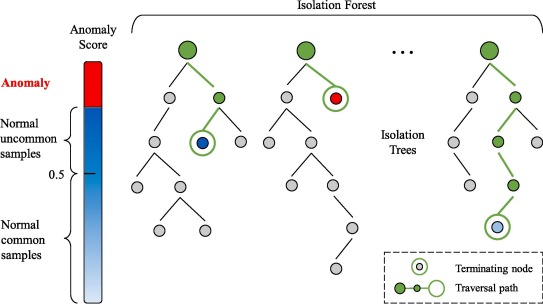
\includegraphics[width=10cm]{fig/Isolation_Forests} % not necessary to give extension - now you can shift between compiling to ps or to pdf without any problems
	
	\caption[Isolation Forest]{Isolation Forests \cite{Chen2020}}
	\label{Figure-Isolation_Forest} 
\end{figure}

The anomaly score is calculated with Eq~\ref{Eq-Isolation_anomaly}
\begin{equation}
	s(x,n) = 2^{-E(h(x))/c(n)}
	\label{Eq-Isolation_anomaly}
\end{equation}
where $E(h(x))$ is the average value of the distance measured from the tree top for a single data point in all the trees \cite{Hariri2021} and $n$ is the size of a data sample used to train a single tree. For the distance to be normalized, $c(n)$ --- the mean distance from the tree top in an unsuccessful search in a \emph{Binary Search Tree} (BST) --- is used and is calculated as 
\begin{equation}
	c(n) = 2H(n-1) - \frac{2(n-1)}{n}.
	\label{Eq-normalizing_isolation}
\end{equation}
$H(i)$ in Eq~\ref{Eq-normalizing_isolation} is the harmonic number and is estimated with Euler's constant as 
\begin{equation}
	H(i) \approx ln(i) + 0.5772156649.
	\label{Eq-H_i}
\end{equation}
Isolation Forests, however have multiple issues, since it splits data in rectangles as seen in Figure~\subref{Figure-ExtendedvsNormal_first}. This is due to the slicing algorithm selecting a feature, $x$ and a cut-off value, $v$. Consequently, the data is either split vertically or horizontally --- if seen as a two dimensional dataset. This split method is unable to categorise complex data structures. These issues however are addressed by \cite{Hariri2021} and led to the \emph{Extended Isolation Forest} algorithm.

The extended isolation forest algorithm generalises the isolation forest algorithm by applying a slope to each slice. Data points are therefore divided into two groups depending on the "side" of the plane or slice as seen in Figure~\subref{Figure-ExtendedvsNormal_second}.

\begin{figure}[h!tb]
	\centering
	
	\subfloat[][Isolation Forest Slicing example]{
		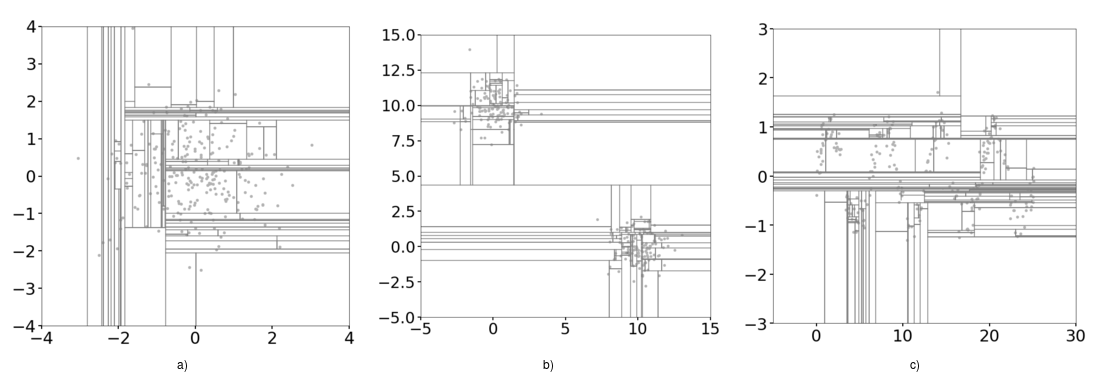
\includegraphics[trim = 0 0 725 0, clip = true, width=7cm]{fig/Isolation_forest_slicing}
		\label{Figure-ExtendedvsNormal_first}
	}
	\quad
	\subfloat[][Extended Isolation Forest Slicing example]{
		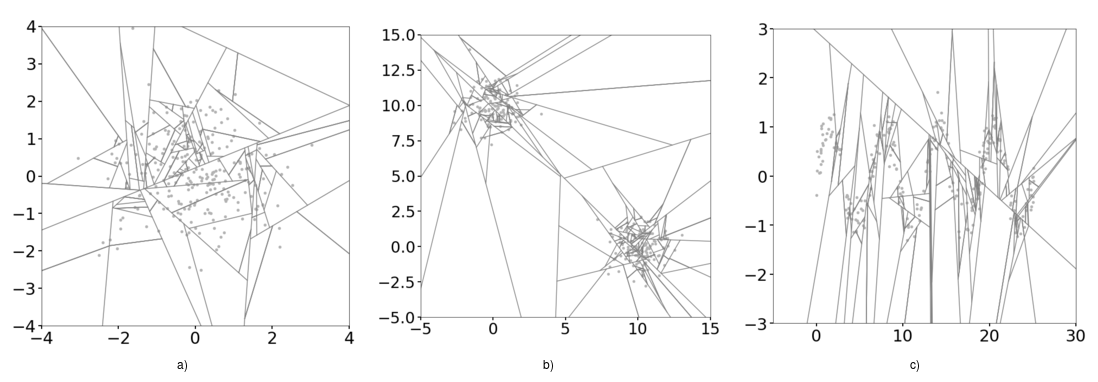
\includegraphics[trim = 0 0 725 0, clip=true,width=7cm]{fig/Extended_Isolation_forest_slicing}
		\label{Figure-ExtendedvsNormal_second}
	}
	\caption[Slicing of Isolation Forest]{The slicing of Isolation Forest vs Extended Isolation Forest}
	\label{Figure-ExtendedvsNormal}
\end{figure}

It is evident that applying an angle of $0\degree$ to all the slices the general algorithm of the extended isolation forest produces the standard isolation forest algorithm where planes or slices are perpendicular to the axis of the randomly selected feature, $x$.

\subsection{Local Outlier Factor}
Most algorithms for anomaly detection are based on a metric which accounts for the entire dataset~\cite{breunig2000lof}. However, many anomalies are identifiable in relation to the local neighbourhood of data points and not the overall dataset. Therefore, \cite{breunig2000lof} developed the local outlier factor \(LOF\) algorithm that provides a measure of a data point's "outlierness". This implies that a data point is not classified as an anomaly or not, but a local outlier factor is calculated to determine how much a data point is distantiated from it's $k$-nearest neighbours. This is clearly demonstrated in Figure~\ref{Figure-LOF_measure} where the data points which are clustered together have smaller LOF's than data points which are removed from the highly dense areas.

\begin{figure}[!hbt]
	\centering
	\import{Figures/}{LOF.pgf}
	\caption{Plane perpendicular to $\mathbf{R}_{SE}$ and at center of earth}
	\label{fig:localOutlierFactor}
\end{figure}

To calculate the LOF, the $k$-distance must be calculated and also the local reachability density \(lrd\). The $k$-distance, is the $k^{th}$ ranked $distance(o,p_i)$. Where $distance(o,p_i)$ is the distance between data point $o$ and any data point $p_i$, with $i \in N$, where $N$ is the number of data points within the dataset with a minimum value of $MinPts$. To reduce fluctuations in the $distance(o,p_i)$ the distance between $o$ and $p_i$ is replaced with 
\begin{equation}
	max \{distance(o,p_i), k\text{-distance}\} 
\end{equation}
and will henceforth be referred to as the reachability distance~\cite{breunig2000lof}. The $lrd$ of a data point, $p$, is calculated as 
\begin{equation}
	lrd_{MinPts}(p) = 1/\left(\frac{\sum\limits_{o \in N_{MinPts}(p)}^{} reach\-dist_{MinPts}(p,o)}{|N_{MinPts}(p)|}\right)
	\label{Eq-lrd}
\end{equation}
and denotes "the inverse of the average reachability distance based on the $MinPts$-nearest neighbours of the $p$" --- \cite{breunig2000lof}. Eq~\ref{Eq-lrd} enables the calculation for the $LOF$ of point $p$ as shown in Eq~\ref{Eq-LOF}
\begin{equation}
	LOF_{MinPts}(p) = \frac{\sum\limits_{o \in N_{MinPts}(p)}^{}\frac{lrd_{MinPts}(o)}{lrd_{MinPts}(p)}}{|N_{MinPts}(p)|}
	\label{Eq-LOF}
\end{equation}
The rule of thumb for detecting an outlier is that when the LOF is larger than 1, then the point is considered an outlier with respect to its neighbourhood. This however is not fixed and the threshold can be changed depending on the application.
This method is aimed at producing a measure of the "outlierness" of a data point within a local neighbourhood and not for all the data points. This method will thus be implemented for the satellite anomaly detection, since it will detect anomalies within the two neighbourhoods produced by the eclipse during orbit. This method will also be able to detect measurements of earth sensors, sun sensors and magnetometers that drastically change from the previous orbital data. For example in Fig~\ref{Figure-Satellite_orbit} it is evident that the LOF will be comparatively larger for the red data points, which are anomalies, to the blue data points that are the normal orbit of the satellite.

\begin{figure}[h!tb]
	\centering
	\begin{tikzpicture}
		\begin{axis}[title = Earth Sensor During Multiple Orbits]
			\addplot3 table [x =Earth x, y = Earth y, z=Earth z, col sep=comma, only marks, scatter, blue, fill opacity=0.1, draw opacity = 0]{Data/3D_orbit.csv};
			\addplot3 table [x =Earth_anomaly x, y = Earth_anomaly y, z=Earth_anomaly z, col sep=comma, only marks, scatter, red, fill opacity=0.1, draw opacity = 0]{Data/3D_orbit.csv};
		\end{axis}
		\label{Figure-Satellite_orbit}
	\end{tikzpicture}
\end{figure}

\section{Summary}

\chapter{Isolation}
\label{chap:Isolation}


\section{Decision Trees}
\begin{figure}[!htb]
	\centering
	\import{Figures/TexFigures/Summary/DecisionTrees100/}{Estimation MetricIsolationWithVaryingPredictionAccuracies.pgf}
	
	\caption{Estimation Metric of Decision Trees at varying isolation percentages.}
	\label{fig:DecisionTreesWithVaryingPredictionEstimation}
\end{figure}

%\begin{figure}[!htb]
%	\centering
%	\import{Figures/TexFigures/Summary/DecisionTrees100/}{Isolation AccuracyIsolationWithVaryingPredictionAccuracies.pgf}
%	
%	\caption{Isolation Accuracy of Decision Trees at varying isolation percentages.}
%	\label{fig:DecisionTreesWithVaryingPredictionIsolation}
%\end{figure}

\section{Random Forests}
\begin{figure}[!htb]
	\centering
	\import{Figures/TexFigures/Summary/RandomForest100/}{Estimation MetricIsolationWithVaryingPredictionAccuracies.pgf}
	
	\caption{Estimation Metric of Random Forest at varying isolation percentages.}
	\label{fig:RandomForestWithVaryingPredictionEstimation}
\end{figure}

%\begin{figure}[!htb]
%	\centering
%	\import{Figures/TexFigures/Summary/RandomForest100/}{Isolation AccuracyIsolationWithVaryingPredictionAccuracies.pgf}
%	
%	\caption{Isolation Accuracy of Random Forest at varying isolation percentages.}
%	\label{fig:RandomForestWithVaryingPredictionIsolation}
%\end{figure}

\section{Support Vector Machines}
\begin{figure}[!htb]
	\centering
	\import{Figures/TexFigures/Summary/SVM/}{Estimation MetricIsolationWithVaryingPredictionAccuracies.pgf}
	
	\caption{Estimation Metric of Support Vector Machines at varying isolation percentages.}
	\label{fig:SVMWithVaryingPredictionEstimation}
\end{figure}

%\begin{figure}[!htb]
%	\centering
%	\import{Figures/TexFigures/Summary/SVM/}{Isolation AccuracyIsolationWithVaryingPredictionAccuracies.pgf}
%	
%	\caption{Isolation Accuracy of Support Vector Machines at varying predictions percentages.}
%	\label{fig:SVMWithVaryingPredictionIsolation}
%\end{figure}

\section{Comparison}
\begin{figure}[!htb]
	\centering
	\import{Figures/TexFigures/Summary/100.0/}{Estimation MetricPerfectPredictionCompareIsolations.pgf}
	
	\caption{Comparison of Estimation Metric of Isolation Methods with a detection accuracy of $100\%$.}
	\label{fig:IsolationMethodsWithPerfectPrediction}
\end{figure}

\section{Summary}
\chapter{Results}
\label{chap:Results}


\section{Perfect Extended Kalman Filter}
For all these results the best recovery method will be demonstrated

\section{Unsupervised Detection and Supervised Isolation}
\begin{figure}[!htb]
	\centering
	\import{Figures/TexFigures/Summary/RandomForest100/}{Estimation MetricReflectionBest.pgf}
	
	\caption{Estimation Metric for recovery methods}
	\label{fig:RecoveryComparisonMagnetic}
\end{figure}

\begin{figure}[!htb]
	\centering
	\import{Figures/TexFigures/Summary/DecisionTrees100/}{Estimation MetricReflectionBest.pgf}
	
	\caption{Estimation Metric for recovery methods}
	\label{fig:RecoveryComparisonMagnetic}
\end{figure}

\begin{figure}[!htb]
	\centering
	\import{Figures/TexFigures/Summary/SVM/}{Estimation MetricReflectionBest.pgf}
	
	\caption{Estimation Metric for recovery methods}
	\label{fig:RecoveryComparisonMagnetic}
\end{figure}

\section{Supervised Detection and Isolation}
Use the best unsupervised learning algorithm from chapter Detection and the best supervised learning algorithm from chapter Isolation

\section{Summary}
\chapter{Conclusion}
\label{chap:Conclusion}


% Bibliography
\bibliography{bibliography.bib}

% End matter
\appendix
\chapter{System Perturbation Matrix}
\makeatletter\@mkboth{}{Appendix}\makeatother
\label{appen:derivations_bigramseg}

This section will show the derivation of the Jacobian matrix $\mathbf{F}_{t}$ that must be constructed in the execution of the full state EKF, as described in Section 5.4.

The continuous system perturbation matrix $\mathbf{F}_{t}$ can be constructed by determining its individual components, thus
$$
\mathbf{F}_{t}=\left[\begin{array}{ll}
\frac{\partial \dot{\omega}_{\mathcal{B}}^{\mathcal{I}}}{\partial \omega_{\mathcal{B}}^{\mathcal{I}}} & \frac{\partial \dot{\omega}_{\mathcal{B}}^{\mathcal{I}}}{\partial \mathbf{q}} \\
\frac{\partial \dot{\mathbf{q}}}{\partial \omega_{\mathcal{B}}^{\mathcal{I}}} & \frac{\partial \dot{\mathbf{q}}}{\partial \mathbf{q}}
\end{array}\right]_{\omega_{\mathcal{B}}^{\mathcal{I}}=\hat{\omega}_{\mathcal{B}}^{\mathcal{I}}, \mathbf{q}=\hat{\mathbf{q}}}
$$
Note that the subscript ' $t$ ' indicating the time domain has been dropped from Equation $5.4 .5$ to simplify the derivation. The non-linear function $\boldsymbol{f}(\mathbf{x})$ can be separated into two parts: a non-linear function describing $\dot{\omega}_{\mathcal{B}}^{\mathcal{I}}$ and a non-linear function describing $\dot{\mathbf{q}}$. The continuous non-linear system equation with regards to $\dot{\omega}_{\mathcal{B}}^{\mathcal{I}}$ is the Euler dynamic equation, or
$$
\dot{\boldsymbol{\omega}}_{\mathcal{B}}^{\mathcal{I}}=\mathbf{J}^{-1}\left(\mathbf{N}_{c}+\mathbf{N}_{d}-\boldsymbol{\omega}_{\mathcal{B}}^{\mathcal{I}} \times\left(\mathbf{J} \boldsymbol{\omega}_{\mathcal{B}}^{\mathcal{I}}+\mathbf{h}_{w}\right)\right)
$$
The individual components of Equation B.2 can also be expressed as
$$
\begin{aligned}
\dot{\omega}_{x i} &=\frac{1}{I_{x x}}\left(N_{c x}+N_{d x}-\omega_{y i}\left(I_{z z} \omega_{z i}+h_{z}\right)+\omega_{z i}\left(I_{y y} \omega_{y i}+h_{y}\right)\right) \\
\dot{\omega}_{y i} &=\frac{1}{I_{y y}}\left(N_{c y}+N_{d y}-\omega_{z i}\left(I_{x x} \omega_{x i}+h_{x}\right)+\omega_{x i}\left(I_{z z} \omega_{z i}+h_{z}\right)\right) \\
\dot{\omega}_{z i} &=\frac{1}{I_{z z}}\left(N_{c z}+N_{d z}-\omega_{x i}\left(I_{y y} \omega_{y i}+h_{y}\right)+\omega_{y i}\left(I_{x x} \omega_{x i}+h_{x}\right)\right) .
\end{aligned}
$$
Using Equations B.3 to B.5, $\frac{\partial \dot{\omega}_{\mathcal{B}}^{\mathcal{I}}}{\partial \omega_{\mathcal{B}}^{\mathcal{I}}}$ can be determined by taking each individual partial derivative, which delivers
$$
\frac{\partial \dot{\boldsymbol{\omega}}_{\mathcal{B}}^{\mathcal{I}}}{\partial \boldsymbol{\omega}_{\mathcal{B}}^{\mathcal{I}}}=\left[\begin{array}{ccc}
0 & \frac{\omega_{z i}\left(I_{y y}-I_{z z}\right)-h_{z}}{I_{x x}} & \frac{\omega_{y i}\left(I_{y y}-I_{z z}\right)+h_{y}}{I_{x x}} \\
\frac{\omega_{z i}\left(I_{z z}-I_{x x}\right)+h_{z}}{I_{y y}} & 0 & \frac{\omega_{x i}\left(I_{z z}-I_{x x}\right)-h_{x}}{I_{y y}} \\
\frac{\omega_{y i}\left(I_{x x}-I_{y y}\right)-h_{y}}{I_{z z}} & \frac{\omega_{x i}\left(I_{x x}-I_{y y}\right)+h_{x}}{I_{z z}} & 0
\end{array}\right] .
$$
$\frac{\partial \dot{\boldsymbol{\omega}}_{\mathcal{B}}^{\mathcal{I}}}{\partial \mathbf{q}}$ is however much more difficult to determine. The first step is to determine which components of Equation B.2 are dependent on the attitude quaternion of the satellite. The control torque $\mathbf{N}_{c}$ is the sum of the torques generated by the ADCS actuators, which means that $\mathbf{N}_{c}$ is independent of $\mathbf{q}$. $\mathbf{N}_{\text {gyro }}$ is calculated using only the moment of inertia matrix, the angular rates and the stored angular momentum, which means that $\mathbf{N}_{\text {gyro }}$ is also independent of $\mathbf{q}$. Although there are many sources of disturbance torques, $\mathbf{N}_{d}$ at a LEO orbit is simplified to contain only two major components, namely gravity gradient torque $\left(\mathbf{N}_{g g}\right)$ and aerodynamic torque $\left(\mathbf{N}_{a e r o}\right)$. Even though both these components are dependent on the attitude of the satellite, only $\mathbf{N}_{g g}$ can be calculated accurately, thus
$$
\mathbf{N}_{d} \approx \mathbf{N}_{g g}
$$
$\mathbf{N}_{d}$ can thus easily be expressed in terms of quaternions using Equation $2.3 .3$ as
$$
\begin{aligned}
&\mathrm{N}_{d x} \approx k_{g x}\left(2\left[q_{2} q_{3}+q_{1} q_{4}\right]\right)\left(-q_{1}^{2}-q_{2}^{2}+q_{3}^{2}+q_{4}^{2}\right) \\
&\mathrm{N}_{d y} \approx k_{g y}\left(2\left[q_{1} q_{3}-q_{2} q_{4}\right]\right)\left(-q_{1}^{2}-q_{2}^{2}+q_{3}^{2}+q_{4}^{2}\right) \\
&\mathrm{N}_{d z} \approx k_{g z}\left(2\left[q_{1} q_{3}-q_{2} q_{4}\right]\right)\left(2\left[q_{2} q_{3}+q_{1} q_{4}\right]\right)
\end{aligned}
$$
$\frac{\partial \dot{\omega}_{\mathcal{B}}^{\mathcal{I}}}{\partial \mathbf{q}}$ can now be calculated as
$$
\frac{\partial \dot{\boldsymbol{\omega}}_{\mathcal{B}}^{\mathcal{I}}}{\partial \mathbf{q}}=\mathbf{J}^{-1}\left[\frac{\partial \mathbf{N}_{d}}{\partial \mathbf{q}}\right]=\mathbf{K}\left[\begin{array}{llll}
\mathbf{d}_{1} & \mathbf{d}_{2} & \mathbf{d}_{3} & \mathbf{d}_{4}
\end{array}\right]
$$
where
$$
\mathbf{K}=\left[\begin{array}{ccc}
2 k_{g x} & 0 & 0 \\
0 & 2 k_{g y} & 0 \\
0 & 0 & 2 k_{g z}
\end{array}\right]
$$
and

$\frac{\partial \dot{\mathbf{q}}}{\partial \boldsymbol{\omega}_{\mathcal{B}}^{\mathcal{I}}}$ and $\frac{\partial \dot{\mathbf{q}}}{\partial \mathbf{q}}$ can be determined by partially deriving the time derivative of $\mathbf{q}$, which is

$$\dot{\mathbf{q}} = \frac{1}{2} \boldsymbol{\Omega}(\omega_{\mathcal{B}}^{\mathcal{O}}) \mathbf{q},$$

where $$\boldsymbol{\Omega}(\omega_{\mathcal{B}}^{\mathcal{O}}) = \begin{bmatrix}
	0 & \omega_{zo} & -\omega_{yo} & \omega_{xo} \\
	-\omega_{zo} & 0 & \omega_{xo} & \omega{yo} \\
	\omega_{yo} & -\omega{xo} & 0 & \omega_{zo} \\
	-\omega_{xo} & -\omega_{yo} & -\omega_{zo} & 0 \\
\end{bmatrix}$$

The relationship between $\omega_{\mathcal{B}}^{\mathcal{I}}$ and $\omega_{\mathcal{B}}^{\mathcal{O}}$ is given by
$$
\boldsymbol{\omega}_{\mathcal{B}}^{\mathcal{O}}=\boldsymbol{\omega}_{\mathcal{B}}^{\mathcal{I}}-\mathbf{A}\left[\begin{array}{c}
0 \\
-\omega_{o} \\
0
\end{array}\right]=\left[\begin{array}{c}
\omega_{x i}+\omega_{o} A_{12} \\
\omega_{y i}+\omega_{o} A_{22} \\
\omega_{z i}+\omega_{o} A_{32}
\end{array}\right]
$$
which means that $\frac{\partial \dot{q}}{\partial \omega_{\mathcal{B}}^{\mathcal{I}}}$ can be determined as
$$
\frac{\partial \dot{\mathbf{q}}}{\partial \omega_{\mathcal{B}}^{\mathcal{I}}}=\left[\begin{array}{ccc}
\frac{\partial \dot{q}_{1}}{\partial \omega_{x i}} & \frac{\partial \dot{q}_{1}}{\partial \omega_{y i}} & \frac{\partial \dot{q}_{1}}{\partial \omega_{z i}} \\
\frac{\partial \dot{q}_{2}}{\partial \omega_{x i}} & \frac{\partial \dot{q}_{2}}{\partial \omega_{y i}} & \frac{\partial \dot{q}_{2}}{\partial \omega_{z i}} \\
\frac{\partial \dot{q}_{3}}{\partial \omega_{x i}} & \frac{\partial \dot{q}_{3}}{\partial \omega_{y i}} & \frac{\partial \dot{q}_{3}}{\partial \omega_{z i}} \\
\frac{\partial \dot{q}_{4}}{\partial \omega_{x i}} & \frac{\partial \dot{q}_{4}}{\partial \omega_{y i}} & \frac{\partial \dot{q}_{4}}{\partial \omega_{z i}}
\end{array}\right]=\frac{1}{2}\left[\begin{array}{ccc}
\hat{q}_{4} & -\hat{q}_{3} & \hat{q}_{2} \\
\hat{q}_{3} & \hat{q}_{4} & -\hat{q}_{1} \\
-\hat{q}_{2} & \hat{q}_{1} & \hat{q}_{4} \\
-\hat{q}_{1} & -\hat{q}_{2} & -\hat{q}_{3}
\end{array}\right]
$$
$\frac{\partial \dot{\mathbf{q}}}{\partial \mathbf{q}}$ can be determined by substituting Equation B.13 into Equation B.12, which delivers
$$
\begin{aligned}
\dot{q}_{1} &=\frac{1}{2}\left(q_{2}\left(\omega_{z i}-\omega_{o} A_{32}\right)-q_{3}\left(\omega_{y i}-\omega_{o} A_{22}\right)+q_{4}\left(\omega_{x i}-\omega_{o} A_{12}\right)\right) \\
\dot{q}_{2} &=\frac{1}{2}\left(-q_{1}\left(\omega_{z i}-\omega_{o} A_{32}\right)+q_{3}\left(\omega_{x i}-\omega_{o} A_{12}\right)+q_{4}\left(\omega_{y i}-\omega_{o} A_{22}\right)\right) \\
\dot{q}_{3} &=\frac{1}{2}\left(q_{1}\left(\omega_{y i}-\omega_{o} A_{22}\right)-q_{2}\left(\omega_{x i}-\omega_{o} A_{12}\right)+q_{4}\left(\omega_{z i}-\omega_{o} A_{32}\right)\right) \\
\dot{q}_{4} &=\frac{1}{2}\left(-q_{1}\left(\omega_{x i}-\omega_{o} A_{12}\right)-q_{2}\left(\omega_{y i}-\omega_{o} A_{22}\right)-q_{3}\left(\omega_{z i}-\omega_{o} A_{32}\right)\right)
\end{aligned}
$$
$$
\begin{aligned}
& \mathbf{d}_{1}=\left[\begin{array}{c}\frac{-q_{1} A_{23}+q_{4} A_{33}}{I_{x x}} \\\frac{-q_{1} A_{13}+q_{3} A_{33}}{I_{y y}} \\\frac{q_{3} A_{23}+q_{4} A_{13}}{I_{z z}}\end{array}\right] \quad \mathbf{d}_{2}=\left[\begin{array}{l}\frac{-q_{2} A_{23}+q_{3} A_{33}}{I_{x x}} \\\frac{-q_{2} A_{13}-q_{4} A_{33}}{I_{y y}} \\\frac{-q_{4} A_{23}+q_{3} A_{13}}{I_{z z}}\end{array}\right] \\
& \mathbf{d}_{3}=\left[\begin{array}{c}\frac{q_{3} A_{23}+q_{2} A_{33}}{I_{x x}} \\\frac{q_{3} A_{13}+q_{1} A_{33}}{I_{y y}} \\\frac{q_{1} A_{23}+q_{2} A_{13}}{I_{z z}}\end{array}\right] \quad \mathbf{d}_{4}=\left[\begin{array}{c}\frac{q_{4} A_{23}+q_{1} A_{33}}{I_{x x}} \\\frac{q_{4} A_{13}-q_{2} A_{33}}{I_{y y}} \\\frac{-q_{2} A_{23}+q_{1} A_{13}}{I_{z z}}\end{array}\right] . 
\end{aligned}
$$
By partially deriving Equations B.15 to B.18 and performing some mathematical manipulation, $\frac{\partial \dot{\mathbf{q}}}{\partial \mathbf{q}}$ can be calculated as
$$
\frac{\partial \dot{\mathbf{q}}}{\partial \mathbf{q}}=\frac{1}{2}\left[\Omega\left(\boldsymbol{\omega}_{\mathcal{B}}^{\mathcal{O}}\right)\right]+\omega_{o}\left[\begin{array}{cccc}
\hat{q}_{1} \hat{q}_{3} & \hat{q}_{1} \hat{q}_{4} & 1-\hat{q}_{1}^{2} & -\hat{q}_{1} \hat{q}_{2} \\
\hat{q}_{2} \hat{q}_{3} & \hat{q}_{2} \hat{q}_{4} & -\hat{q}_{1} \hat{q}_{2} & 1-\hat{q}_{2}^{2} \\
-\left(1-\hat{q}_{3}^{2}\right) & \hat{q}_{3} \hat{q}_{4} & -\hat{q}_{1} \hat{q}_{3} & -\hat{q}_{2} \hat{q}_{3} \\
\hat{q}_{3} \hat{q}_{4} & -\left(1-\hat{q}_{4}^{2}\right) & -\hat{q}_{1} \hat{q}_{4} & -\hat{q}_{2} \hat{q}_{4}
\end{array}\right]
$$

\chapter{Measurement Perturbation Jacobian Matrix}
\makeatletter\@mkboth{}{Appendix}\makeatother
\label{chap:Measurement Perturbation Jacobian Matrix}
This section will show the derivation of the Jacobian matrix $\mathbf{H}_{k}$ that must be constructed in the execution of the full state $\mathrm{EKF}$, as described in Section $5.4 .$

The discrete measurement perturbation matrix $\mathbf{H}_{k}$ from Equation $5.4 .12$ can be determined by partially deriving the non-linear function $\boldsymbol{h}\left(\mathbf{x}_{k}\right)$, which is given by Equation $5.4 .15$ as
$$
\boldsymbol{h}\left(\mathbf{x}_{k}\right)=\mathbf{A} \mathbf{v}_{\mathcal{O}_k} .
$$
Since $\mathbf{A}$ is constructed from $\mathbf{q}$ only, Equation B.20 suggests that $\boldsymbol{h}\left(\mathbf{x}_{k}\right)$ is independent of $\boldsymbol{\omega}_{\mathcal{B}}^{\mathcal{I}}$, thus
$$
\mathbf{H}_{k}=\left[\begin{array}{lllllll}
0 & 0 & 0 & \frac{\partial h_{1}}{\partial q_{1}} & \frac{\partial h_{1}}{\partial q_{2}} & \frac{\partial h_{1}}{\partial q_{3}} & \frac{\partial h_{1}}{\partial q_{4}} \\
0 & 0 & 0 & \frac{\partial h_{2}}{\partial q_{1}} & \frac{\partial h_{2}}{\partial q_{2}} & \frac{\partial h_{2}}{\partial q_{3}} & \frac{\partial h_{2}}{\partial q_{4}} \\
0 & 0 & 0 & \frac{\partial h_{3}}{\partial q_{1}} & \frac{\partial h_{3}}{\partial q_{2}} & \frac{\partial h_{3}}{\partial q_{3}} & \frac{\partial h_{3}}{\partial q_{4}}
\end{array}\right]_{\mathbf{q}=\hat{\mathbf{q}}}
$$
$\mathbf{H}_{k}$ can thus be calculated as
$$
\mathbf{H}_{k}=\left[\begin{array}{lllll}
\mathbf{0}_{[3 \times 3]} & \mathbf{h}_{1} & \mathbf{h}_{2} & \mathbf{h}_{3} & \mathbf{h}_{4}
\end{array}\right] \text {, }
$$
where $\quad \mathbf{h}_{1}=2\left[\begin{array}{ccc}q_{1} & q_{2} & q_{3} \\ q_{2} & -q_{1} & q_{4} \\ q_{3} & -q_{4} & -q_{1}\end{array}\right] \mathbf{v}_{\mathcal{O}_k}$,
$$
\mathbf{h}_{2}=2\left[\begin{array}{ccc}
-q_{2} & q_{1} & -q_{4} \\
q_{1} & q_{2} & q_{3} \\
q_{4} & q_{3} & -q_{2}
\end{array}\right] \mathbf{v}_{\mathcal{O}_k}
$$
$\mathbf{h}_{3}=2\left[\begin{array}{ccc}-q_{3} & q_{4} & q_{1} \\ -q_{4} & -q_{3} & q_{2} \\ q_{1} & q_{2} & q_{3}\end{array}\right] \mathbf{v}_{\mathcal{O}_k}$

and $\quad \mathbf{h}_{4}=2\left[\begin{array}{ccc}q_{4} & q_{3} & -q_{2} \\ -q_{3} & q_{4} & q_{1} \\ q_{2} & -q_{1} & q_{4}\end{array}\right] \mathbf{v}_{\mathcal{O}_k}$

\chapter{System Noise Covariance Matrix}
\makeatletter\@mkboth{}{Appendix}\makeatother
\label{chap:System Noise Covariance Matrix}
This section will show the derivation of the covariance matrix $\mathbf{Q}_{k}$ that must be constructed in the execution of the full state EKF, as described in Section $5.4 .$

The system noise covariance matrix $\mathbf{Q}_{k}$ can easily be determined from the continuous domain system noise covariance matrix $\mathbf{Q}_{t}$ if the following assumptions are made:

\begin{itemize}
	\item The angular rate noise (due to unmodelled disturbance torques and modelling errors) is uncorrelated.
	
	\item The system noise is small enough to allow the state matrix $\boldsymbol{\Phi}_{k}$ to be approximated using only two terms without significant inaccuracies, thus $\mathbf{\Phi}_{k} \approx \mathbf{I}+\left[T_{s} \mathbf{F}_{t}\right]_{t=k T_{s}}$.
	
	\item The angular rate noise for each axis is equal, thus $\sigma_{\omega x}=\sigma_{\omega y}=\sigma_{\omega z}=\sigma_{\omega}$.
	
\end{itemize}
Given the above-mentioned assumptions, the angular rate noise covariance matrix $\mathbf{Q}_{\omega, t}$ is given as
$$
\mathbf{Q}_{\omega, t}=\left[\begin{array}{ccc}
\sigma_{\omega}^{2} & 0 & 0 \\
0 & \sigma_{\omega}^{2} & 0 \\
0 & 0 & \sigma_{\omega}^{2}
\end{array}\right]
$$
$\mathbf{q}$ is completely described by the equations in Section 5.4, which means that the noise covariance of the last four states of the system $\left(\mathbf{Q}_{q, t}\right)$ is simply a zero matrix, or
$$
\mathbf{Q}_{q, t}=\mathbf{0}_{[4 \times 4]}
$$
$\mathbf{Q}_{t}$ can be formed from Equations B.23 and B.24 as
$$
\begin{aligned}
\mathbf{Q}_{t} &=\left[\begin{array}{ll}
\mathbf{Q}_{\omega, t} & \mathbf{0}_{[3 \times 4]} \\
\mathbf{0}_{[4 \times 3]} & \mathbf{Q}_{q, t}
\end{array}\right] \\
&=\left[\begin{array}{ll}
\mathbf{Q}_{\omega, t} & \mathbf{0}_{[3 \times 4]} \\
\mathbf{0}_{[4 \times 3]} & \mathbf{0}_{[4 \times 4]}
\end{array}\right]
\end{aligned}
$$
$\mathbf{F}_{t}$ can also be express in the form of Equation B.26 as
$$
\mathbf{F}_{t}=\left[\begin{array}{ll}
\mathbf{F}_{11[3 \times 3]} & \mathbf{F}_{12[3 \times 4]} \\
\mathbf{F}_{21[4 \times 3]} & \mathbf{F}_{22[4 \times 4]}
\end{array}\right]
$$
$\mathbf{Q}_{k}$ can now be determined by converting $\mathbf{Q}_{t}$ to the discrete domain. Through a process of integration $[21], \mathbf{Q}_{k}$ is determined to be
$$
\mathbf{Q}_{k}=T_{s} \mathbf{S}_{1}+\frac{1}{2} T_{s}^{2} \mathbf{S}_{2}+\frac{1}{3} T_{s}^{3} \mathbf{S}_{3}
$$
where $\mathbf{S}_{1}=\mathbf{Q}_{t}$
$$
\begin{aligned}
&\mathbf{S}_{2}=\left[\begin{array}{cc}
\mathbf{Q}_{\omega, t} \mathbf{F}_{11}^{T}+\mathbf{F}_{11} \mathbf{Q}_{\omega, t} & \mathbf{Q}_{\omega, t} \mathbf{F}_{21}^{T} \\
\mathbf{F}_{21} \mathbf{Q}_{\omega, t} & \mathbf{0}_{[4 \times 4]}
\end{array}\right]_{t=k T_{s}} \\
&\mathbf{S}_{3}=\left[\begin{array}{ll}
\mathbf{F}_{11} \mathbf{Q}_{\omega, t} \mathbf{F}_{11}^{T} & \mathbf{F}_{11} \mathbf{Q}_{\omega, t} \mathbf{F}_{21}^{T} \\
\mathbf{F}_{21} \mathbf{Q}_{\omega, t} \mathbf{F}_{11}^{T} & \mathbf{F}_{21} \mathbf{Q}_{\omega, t} \mathbf{F}_{21}^{T}
\end{array}\right]_{t=k T_{s}}
\end{aligned}
$$
The computational load of calculating $\mathbf{Q}_{k}$ can be reduced if the assumption is made that $\mathbf{F}_{11}<<\mathbf{F}_{21}$ [21]. $\mathbf{Q}_{k}$ can then be simplified to
$$
\mathbf{Q}_{k}=\left[\begin{array}{cc}
T_{s} \mathbf{Q}_{\omega, t} & \frac{1}{2} T_{s}{ }^{2} \mathbf{Q}_{\omega, t} \mathbf{F}_{21}^{T} \\
\frac{1}{2} T_{s}{ }^{2} \mathbf{F}_{21} \mathbf{Q}_{\omega, t} & \frac{1}{3} T_{s}{ }^{3} \mathbf{F}_{21} \mathbf{Q}_{\omega, t} \mathbf{F}_{21}^{T}
\end{array}\right]_{t=k T_{s}}
$$

\chapter{Measurement Noise Covariance Matrix}
\makeatletter\@mkboth{}{Appendix}\makeatother
\label{chap:Measurement Noise Covariance Matrix}
This section will show the derivation of the covariance matrix $\mathbf{R}_{k}$ that must be constructed in the execution of the full state EKF, as described in Section 5.4.

The relationship between the true measured vector $\overline{\mathbf{v}}_{\mathcal{B}_k}$ and the true modelled vector $\overline{\mathbf{v}}_{\mathcal{O}_k}$ is given by Equation $5.4 .13$ as
$$
\overline{\mathbf{v}}_{\mathcal{B}_k}=\mathbf{A}\left(\mathbf{q}_{k}\right) \overline{\mathbf{v}}_{\mathcal{O}_k} .
$$
It should be noted that $\mathbf{A}_{k}=\mathbf{A}\left(\mathbf{q}_{k}\right)$. The added notation, which merely implies that $\mathbf{A}$ is a function of $\mathbf{q}_{k}$, will prove to be useful in the remainder of this section.

The measured and modelled vectors are furthermore related to their respective true vectors through
$$
\begin{aligned}
\mathbf{v}_{\mathcal{B}_k} &=\overline{\mathbf{v}}_{\mathcal{B}_k}+\mathbf{m}_{\mathcal{B}_k} \\
\text { and } \quad \mathbf{v}_{\mathcal{O}_k} &=\overline{\mathbf{v}}_{\mathcal{O}_k}+\mathbf{m}_{\mathcal{O}_k}
\end{aligned}
$$
If $\Delta \mathbf{q}_{k}$ is defined as the difference between the true quaternion $\mathbf{q}_{k}$ and the estimated quaternion $\hat{\mathbf{q}}_{k}$,
$$
\Delta \mathbf{q}_{k}=\mathbf{q}_{k}-\hat{\mathbf{q}}_{k}
$$
then Equation $5.4 .13$ can also be expressed as
$$
\mathbf{v}_{\mathcal{B}_k}-\mathbf{m}_{\mathcal{B}_k}=\mathbf{A}\left(\hat{\mathbf{q}}_{k}+\Delta \mathbf{q}_{k}\right)\left(\mathbf{v}_{\mathcal{O}_k}-\mathbf{m}_{\mathcal{O}_k}\right)
$$
The Taylor series expansion from Equations $5.4 .4$ and $5.4 .11$ can also be used to approximate $\mathbf{A}\left(\hat{\mathbf{q}}_{k}+\right.$ $\left.\Delta \mathbf{q}_{k}\right)$ as
$$
\begin{aligned}
&\mathbf{A}\left(\hat{\mathbf{q}}_{k}+\Delta \mathbf{q}_{k}\right) \approx \mathbf{A}\left(\hat{\mathbf{q}}_{k}\right)+\mathbf{C}_{k} \Delta \mathbf{q}_{k} \\
&\text { where } \quad \mathbf{C}_{k}=\left[\frac{\partial \mathbf{A}\left(\hat{\mathbf{q}}_{k}\right)}{\partial \hat{\mathbf{q}}_{k}}\right]
\end{aligned}
$$
Substituting Equation B.37 into Equation B.36 delivers
$$
\mathbf{v}_{\mathcal{B}_k}-\mathbf{m}_{\mathcal{B}_k}=\left(\mathbf{A}\left(\hat{\mathbf{q}}_{k}\right)+\mathbf{C}_{k} \Delta \mathbf{q}_{k}\right)\left(\mathbf{v}_{\mathcal{O}_k}-\mathbf{m}_{\mathcal{O}_k}\right)
$$
Given that the innovation $\mathbf{e}_{k}$ is defined by Equation $5.4 .17$ as
$$
\mathbf{e}_{k}=\mathbf{v}_{\mathcal{B}_k}-\mathbf{A}\left(\hat{\mathbf{q}}_{k}\right) \mathbf{v}_{\mathcal{O}_k},
$$
substitution can be used to manipulate Equation B.39 into
$$
\mathbf{e}_{k}=\left(\mathbf{C}_{k} \mathbf{v}_{\mathcal{O}_k}-\mathbf{C}_{k} \mathbf{m}_{\mathcal{O}_k}\right) \Delta \mathbf{q}_{k}+\mathbf{m}_{\mathcal{B}_k}-\mathbf{A}\left(\hat{\mathbf{q}}_{k}\right) \mathbf{m}_{\mathcal{O}_k}
$$
If it is assumed that $\mathbf{m}_{\mathcal{O}_k}$ and $\Delta \mathbf{q}_{k}$ are extremely small compared respectively to $\mathbf{v}_{m o d e l}, k$ and $\mathbf{q}_{k}$, then
$$
\mathbf{m}_{\mathcal{O}_k} \Delta \mathbf{q}_{k} \approx 0
$$
Equation B. 40 can thus be simplified to
$$
\begin{aligned}
\mathbf{e}_{k} &=\left[\mathbf{0}_{[3 \times 3]} \mathbf{C}_{k} \mathbf{v}_{\mathcal{O}_k}\right] \Delta \mathbf{x}_{k}+\mathbf{m}_{k}, \\
\text { where } \quad \mathbf{m}_{k} &=\mathbf{m}_{\mathcal{B}_k}-\mathbf{A}\left(\hat{\mathbf{q}}_{k}\right) \mathbf{m}_{\mathcal{O}_k}
\end{aligned}
$$
The covariance matrix $\mathbf{R}_{k}$ of $\mathbf{m}_{k}$ is defined as
$$
\begin{aligned}
\mathbf{R}_{k}=& \mathbb{E}\left\{\left(\mathbf{m}_{k}\right)\left(\mathbf{m}_{k}\right)^{T}\right\} \\
=& \mathbb{E}\left\{\left(\mathbf{m}_{\mathcal{B}_k}-\mathbf{A}\left(\hat{\mathbf{q}}_{k}\right) \mathbf{m}_{\mathcal{O}_k}\right)\left(\mathbf{m}_{\mathcal{B}_k}-\mathbf{A}\left(\hat{\mathbf{q}}_{k}\right) \mathbf{m}_{\mathcal{O}_k}\right)^{T}\right\} \\
=& \mathbb{E}\left\{\mathbf{m}_{\mathcal{B}_k} \mathbf{m}_{\mathcal{B}_k}^{T}-\right.\\
& \quad \mathbf{m}_{\mathcal{B}_k} \mathbf{m}_{\mathcal{O}_k}^{T} \mathbf{A}\left(\hat{\mathbf{q}}_{k}\right)^{T}-\\
& \mathbf{A}\left(\hat{\mathbf{q}}_{k}\right) \mathbf{m}_{\mathcal{O}_k} \mathbf{m}_{\mathcal{B}_k}^{T}+\\
&\left.\mathbf{A}\left(\hat{\mathbf{q}}_{k}\right) \mathbf{m}_{\mathcal{O}_k} \mathbf{m}_{\mathcal{O}_k}^{T} \mathbf{A}\left(\hat{\mathbf{q}}_{k}\right)^{T}\right\} \\
=& \mathbb{E}\left\{\mathbf{m}_{\mathcal{B}_k} \mathbf{m}_{\mathcal{B}_k}^{T}\right\}-\\
& \mathbb{E}\left\{\mathbf{m}_{\mathcal{B}_k} \mathbf{m}_{\mathcal{O}_k}^{T} \mathbf{A}\left(\hat{\mathbf{q}}_{k}\right)^{T}\right\}-\\
& \mathbb{E}\left\{\mathbf{A}\left(\hat{\mathbf{q}}_{k}\right) \mathbf{m}_{\mathcal{O}_k} \mathbf{m}_{\mathcal{B}_k}^{T}\right\}+\\
& \mathbb{E}\left\{\mathbf{A}\left(\hat{\mathbf{q}}_{k}\right) \mathbf{m}_{\mathcal{O}_k} \mathbf{m}_{\mathcal{O}_k}^{T} \mathbf{A}\left(\hat{\mathbf{q}}_{k}\right)^{T}\right\}
\end{aligned}
$$
where $\mathbb{E}$ indicates the expected value operator. The last term of Equation B.44 can be simplified to
$$
\mathbf{A}\left(\hat{\mathbf{q}}_{k}\right) \mathbf{m}_{\mathcal{O}_k} \mathbf{m}_{\mathcal{O}_k} T \mathbf{A}\left(\hat{\mathbf{q}}_{k}\right)^{T}=\mathbf{m}_{\mathcal{O}_k} \mathbf{m}_{\mathcal{O}_k}^{T}
$$
since $\mathbf{m}_{\mathcal{O}_k} \mathbf{m}_{\mathcal{O}_k}^{T}$ is a scalar value and $\mathbf{A}\left(\hat{\mathbf{q}}_{k}\right) \mathbf{A}\left(\hat{\mathbf{q}}_{k}\right)^{T}=1$. If it is furthermore assumed that the measurement noise and the model noise are uncorrelated and that each noise vector has equal variance in its 3 axes, then Equation B. 44 becomes
$$
\begin{aligned}
\mathbf{R}_{k}=& \mathbb{E}\left\{\mathbf{m}_{\mathcal{B}_k} \mathbf{m}_{\mathcal{B}_k}^{T}\right\}+\\
& \mathbb{E}\left\{\mathbf{m}_{\mathcal{O}_k} \mathbf{m}_{\mathcal{O}_k}^{T}\right\} \\
=&\left(\sigma_{\mathcal{B}}^{2}+\sigma_{\mathcal{O}}^{2}\right) \mathbf{I}_{3 \times 3}
\end{aligned}
$$
where $\sigma_{\mathcal{B}}$ and $\sigma_{\mathcal{O}}$ are the respective standard deviations of $\mathbf{m}_{\mathcal{B}_k}$ and $\mathbf{m}_{\mathcal{O}_k}$. It is also assumed that $\sigma_{\mathcal{B}}$ and $\sigma_{\mathcal{O}}$ are constant.

\end{document}
